\documentclass[review,screen,acmsmall,anonymous=true]{acmart}
\settopmatter{printfolios=false,printccs=false,printacmref=false}
\setcopyright{none}
\renewcommand\footnotetextcopyrightpermission[1]{}
\pagestyle{plain}


\bibliographystyle{ACM-Reference-Format}
\citestyle{acmauthoryear}   %% For author/year citations
\usepackage{listings,hyperref,multirow,paralist,xspace,url,wrapfig}
\usepackage{tabularx}
\newcommand{\missingTag}[1]{\textcolor{red}{#1}\xspace}
\newcommand{\missingNumber}{\textcolor{red}{XX}\xspace}
\newcommand{\missingPercentage}{\textcolor{red}{XX\%}\xspace}
\newcommand{\missingTable}[1][XX]{\textcolor{red}{Table #1}\xspace}
\newcommand{\missingGraph}{\textcolor{red}{XXGraph}\xspace}


%\newcommand{\CoreEvalCallCountRnd}{12.6M\xspace}
\newcommand{\CoreEvalCallCount}{12,637,139\xspace}
\newcommand{\CoreEvalSiteCountRnd}{170\xspace}
\newcommand{\CoreEvalSiteCount}{170\xspace}
\newcommand{\CoreEvalParentCallCountRnd}{254.1K\xspace}
\newcommand{\CoreEvalParentCallCount}{254,112\xspace}
\newcommand{\CoreEvalParentSiteCountRnd}{16\xspace}
\newcommand{\CoreEvalParentSiteCount}{16\xspace}
\newcommand{\CoreEvalqCallCountRnd}{265.5K\xspace}
\newcommand{\CoreEvalqCallCount}{265,499\xspace}
\newcommand{\CoreEvalqSiteCountRnd}{4\xspace}
\newcommand{\CoreEvalqSiteCount}{4\xspace}
\newcommand{\CoreLocalCallCountRnd}{234.2K\xspace}
\newcommand{\CoreLocalCallCount}{234,212\xspace}
\newcommand{\CoreLocalSiteCountRnd}{1.1K\xspace}
\newcommand{\CoreLocalSiteCount}{1,116\xspace}
\newcommand{\PackageEvalCallCountRnd}{5M\xspace}
\newcommand{\PackageEvalCallCount}{5,021,240\xspace}
\newcommand{\PackageEvalSiteCountRnd}{2.4K\xspace}
\newcommand{\PackageEvalSiteCount}{2,448\xspace}
\newcommand{\PackageEvalParentCallCountRnd}{52.1K\xspace}
\newcommand{\PackageEvalParentCallCount}{52,130\xspace}
\newcommand{\PackageEvalParentSiteCountRnd}{351\xspace}
\newcommand{\PackageEvalParentSiteCount}{351\xspace}
\newcommand{\PackageEvalqCallCountRnd}{292\xspace}
\newcommand{\PackageEvalqCallCount}{292\xspace}
\newcommand{\PackageEvalqSiteCountRnd}{7\xspace}
\newcommand{\PackageEvalqSiteCount}{7\xspace}
\newcommand{\PackageLocalCallCountRnd}{1.3K\xspace}
\newcommand{\PackageLocalCallCount}{1,251\xspace}
\newcommand{\PackageLocalSiteCountRnd}{8\xspace}
\newcommand{\PackageLocalSiteCount}{8\xspace}
\newcommand{\KaggleEvalCallCountRnd}{0\xspace}
\newcommand{\KaggleEvalCallCount}{0\xspace}
\newcommand{\KaggleEvalSiteCountRnd}{0\xspace}
\newcommand{\KaggleEvalSiteCount}{0\xspace}
\newcommand{\KaggleEvalParentCallCountRnd}{0\xspace}
\newcommand{\KaggleEvalParentCallCount}{0\xspace}
\newcommand{\KaggleEvalParentSiteCountRnd}{0\xspace}
\newcommand{\KaggleEvalParentSiteCount}{0\xspace}
\newcommand{\KaggleEvalqCallCountRnd}{0\xspace}
\newcommand{\KaggleEvalqCallCount}{0\xspace}
\newcommand{\KaggleEvalqSiteCountRnd}{0\xspace}
\newcommand{\KaggleEvalqSiteCount}{0\xspace}
\newcommand{\KaggleLocalCallCountRnd}{0\xspace}
\newcommand{\KaggleLocalCallCount}{0\xspace}
\newcommand{\KaggleLocalSiteCountRnd}{0\xspace}
\newcommand{\KaggleLocalSiteCount}{0\xspace}
\newcommand{\CoreAllCallCountRnd}{13.4M\xspace}
\newcommand{\CoreAllCallCount}{13,390,962\xspace}
\newcommand{\CoreAllSiteCountRnd}{1.3K\xspace}
\newcommand{\CoreAllSiteCount}{1,306\xspace}
\newcommand{\KaggleAllCallCountRnd}{0\xspace}
\newcommand{\KaggleAllCallCount}{0\xspace}
\newcommand{\KaggleAllSiteCountRnd}{0\xspace}
\newcommand{\KaggleAllSiteCount}{0\xspace}
\newcommand{\PackageAllCallCountRnd}{5.1M\xspace}
\newcommand{\PackageAllCallCount}{5,074,913\xspace}
\newcommand{\PackageAllSiteCountRnd}{2.8K\xspace}
\newcommand{\PackageAllSiteCount}{2,814\xspace}
\newcommand{\AllEvalCallCountRnd}{17.7M\xspace}
\newcommand{\AllEvalCallCount}{17,658,379\xspace}
\newcommand{\AllEvalSiteCountRnd}{2.6K\xspace}
\newcommand{\AllEvalSiteCount}{2,618\xspace}
\newcommand{\AllEvalParentCallCountRnd}{306.2K\xspace}
\newcommand{\AllEvalParentCallCount}{306,242\xspace}
\newcommand{\AllEvalParentSiteCountRnd}{367\xspace}
\newcommand{\AllEvalParentSiteCount}{367\xspace}
\newcommand{\AllEvalqCallCountRnd}{265.8K\xspace}
\newcommand{\AllEvalqCallCount}{265,791\xspace}
\newcommand{\AllEvalqSiteCountRnd}{11\xspace}
\newcommand{\AllEvalqSiteCount}{11\xspace}
\newcommand{\AllLocalCallCountRnd}{235.5K\xspace}
\newcommand{\AllLocalCallCount}{235,463\xspace}
\newcommand{\AllLocalSiteCountRnd}{1.1K\xspace}
\newcommand{\AllLocalSiteCount}{1,124\xspace}
\newcommand{\AllAllCallCountRnd}{18.5M\xspace}
\newcommand{\AllAllCallCount}{18,465,875\xspace}
\newcommand{\AllAllSiteCountRnd}{4.1K\xspace}
\newcommand{\AllAllSiteCount}{4,120\xspace}
\newcommand{\TotalFileCountRnd}{23.9K\xspace}
\newcommand{\TotalFileCount}{23,871\xspace}
\newcommand{\NoEvalFileCountRnd}{0\xspace}
\newcommand{\NoEvalFileCount}{0\xspace}
\newcommand{\NoEvalFilePerc}{0\%\xspace}
\newcommand{\CoreEvalFileCountRnd}{13.6K\xspace}
\newcommand{\CoreEvalFileCount}{13,584\xspace}
\newcommand{\CoreEvalFilePerc}{56.9\%\xspace}
\newcommand{\PackageEvalFileCountRnd}{224\xspace}
\newcommand{\PackageEvalFileCount}{224\xspace}
\newcommand{\PackageEvalFilePerc}{0.9\%\xspace}
\newcommand{\AllEvalFileCountRnd}{10.1K\xspace}
\newcommand{\AllEvalFileCount}{10,063\xspace}
\newcommand{\AllEvalFilePerc}{42.2\%\xspace}
\newcommand{\EightyCoreEvalFileCountRnd}{5.9K\xspace}
\newcommand{\EightyCoreEvalFileCount}{5,930\xspace}
\newcommand{\EightyCoreEvalFilePerc}{58.9\%\xspace}
\newcommand{\TopTenPackageCallCountRnd}{3.8M\xspace}
\newcommand{\TopTenPackageCallCount}{3,794,346\xspace}
\newcommand{\TopTenPackageCallPerc}{86.5\%\xspace}
\newcommand{\TopTenPackageSiteCountRnd}{169\xspace}
\newcommand{\TopTenPackageSiteCount}{169\xspace}
\newcommand{\TopTenPackageSitePerc}{6.2\%\xspace}
\newcommand{\TopTenPackageNameA}{ggplot2\xspace}
\newcommand{\TopTenPackageCallsiteCountARnd}{2\xspace}
\newcommand{\TopTenPackageCallsiteCountA}{2\xspace}
\newcommand{\TopTenPackageCallCountARnd}{2M\xspace}
\newcommand{\TopTenPackageCallCountA}{2,026,739\xspace}
\newcommand{\TopTenPackageCallPercA}{46.2\%\xspace}
\newcommand{\TopTenPackageNameB}{magrittr\xspace}
\newcommand{\TopTenPackageCallsiteCountBRnd}{6\xspace}
\newcommand{\TopTenPackageCallsiteCountB}{6\xspace}
\newcommand{\TopTenPackageCallCountBRnd}{536K\xspace}
\newcommand{\TopTenPackageCallCountB}{536,016\xspace}
\newcommand{\TopTenPackageCallPercB}{12.2\%\xspace}
\newcommand{\TopTenPackageNameC}{data.table\xspace}
\newcommand{\TopTenPackageCallsiteCountCRnd}{47\xspace}
\newcommand{\TopTenPackageCallsiteCountC}{47\xspace}
\newcommand{\TopTenPackageCallCountCRnd}{229.1K\xspace}
\newcommand{\TopTenPackageCallCountC}{229,073\xspace}
\newcommand{\TopTenPackageCallPercC}{5.2\%\xspace}
\newcommand{\TopTenPackageNameD}{glue\xspace}
\newcommand{\TopTenPackageCallsiteCountDRnd}{9\xspace}
\newcommand{\TopTenPackageCallsiteCountD}{9\xspace}
\newcommand{\TopTenPackageCallCountDRnd}{192.4K\xspace}
\newcommand{\TopTenPackageCallCountD}{192,423\xspace}
\newcommand{\TopTenPackageCallPercD}{4.4\%\xspace}
\newcommand{\TopTenPackageNameE}{brms\xspace}
\newcommand{\TopTenPackageCallsiteCountERnd}{1\xspace}
\newcommand{\TopTenPackageCallsiteCountE}{1\xspace}
\newcommand{\TopTenPackageCallCountERnd}{166.1K\xspace}
\newcommand{\TopTenPackageCallCountE}{166,132\xspace}
\newcommand{\TopTenPackageCallPercE}{3.8\%\xspace}
\newcommand{\TopTenPackageNameF}{copula\xspace}
\newcommand{\TopTenPackageCallsiteCountFRnd}{52\xspace}
\newcommand{\TopTenPackageCallsiteCountF}{52\xspace}
\newcommand{\TopTenPackageCallCountFRnd}{145.8K\xspace}
\newcommand{\TopTenPackageCallCountF}{145,762\xspace}
\newcommand{\TopTenPackageCallPercF}{3.3\%\xspace}
\newcommand{\TopTenPackageNameG}{np\xspace}
\newcommand{\TopTenPackageCallsiteCountGRnd}{23\xspace}
\newcommand{\TopTenPackageCallsiteCountG}{23\xspace}
\newcommand{\TopTenPackageCallCountGRnd}{142K\xspace}
\newcommand{\TopTenPackageCallCountG}{141,967\xspace}
\newcommand{\TopTenPackageCallPercG}{3.2\%\xspace}
\newcommand{\TopTenPackageNameH}{R6\xspace}
\newcommand{\TopTenPackageCallsiteCountHRnd}{1\xspace}
\newcommand{\TopTenPackageCallsiteCountH}{1\xspace}
\newcommand{\TopTenPackageCallCountHRnd}{128.4K\xspace}
\newcommand{\TopTenPackageCallCountH}{128,371\xspace}
\newcommand{\TopTenPackageCallPercH}{2.9\%\xspace}
\newcommand{\TopTenPackageNameI}{plyr\xspace}
\newcommand{\TopTenPackageCallsiteCountIRnd}{17\xspace}
\newcommand{\TopTenPackageCallsiteCountI}{17\xspace}
\newcommand{\TopTenPackageCallCountIRnd}{118.4K\xspace}
\newcommand{\TopTenPackageCallCountI}{118,408\xspace}
\newcommand{\TopTenPackageCallPercI}{2.7\%\xspace}
\newcommand{\TopTenPackageNameJ}{statnet.common\xspace}
\newcommand{\TopTenPackageCallsiteCountJRnd}{11\xspace}
\newcommand{\TopTenPackageCallsiteCountJ}{11\xspace}
\newcommand{\TopTenPackageCallCountJRnd}{109.5K\xspace}
\newcommand{\TopTenPackageCallCountJ}{109,455\xspace}
\newcommand{\TopTenPackageCallPercJ}{2.5\%\xspace}
\newcommand{\SiteSummarySiteCountA}{1\xspace}
\newcommand{\SiteSummaryPackageCountARnd}{89\xspace}
\newcommand{\SiteSummaryPackageCountA}{89\xspace}
\newcommand{\SiteSummarySiteCountB}{2\xspace}
\newcommand{\SiteSummaryPackageCountBRnd}{41\xspace}
\newcommand{\SiteSummaryPackageCountB}{41\xspace}
\newcommand{\SiteSummarySiteCountC}{3\xspace}
\newcommand{\SiteSummaryPackageCountCRnd}{23\xspace}
\newcommand{\SiteSummaryPackageCountC}{23\xspace}
\newcommand{\SiteSummarySiteCountD}{4\xspace}
\newcommand{\SiteSummaryPackageCountDRnd}{19\xspace}
\newcommand{\SiteSummaryPackageCountD}{19\xspace}
\newcommand{\SiteSummarySiteCountE}{5\xspace}
\newcommand{\SiteSummaryPackageCountERnd}{11\xspace}
\newcommand{\SiteSummaryPackageCountE}{11\xspace}
\newcommand{\SiteSummarySiteCountF}{6\xspace}
\newcommand{\SiteSummaryPackageCountFRnd}{20\xspace}
\newcommand{\SiteSummaryPackageCountF}{20\xspace}
\newcommand{\SiteSummarySiteCountG}{7\xspace}
\newcommand{\SiteSummaryPackageCountGRnd}{15\xspace}
\newcommand{\SiteSummaryPackageCountG}{15\xspace}
\newcommand{\SiteSummarySiteCountH}{8\xspace}
\newcommand{\SiteSummaryPackageCountHRnd}{3\xspace}
\newcommand{\SiteSummaryPackageCountH}{3\xspace}
\newcommand{\SiteSummarySiteCountI}{9\xspace}
\newcommand{\SiteSummaryPackageCountIRnd}{7\xspace}
\newcommand{\SiteSummaryPackageCountI}{7\xspace}
\newcommand{\SiteSummarySiteCountJ}{10\xspace}
\newcommand{\SiteSummaryPackageCountJRnd}{3\xspace}
\newcommand{\SiteSummaryPackageCountJ}{3\xspace}
\newcommand{\SiteSummarySiteCountK}{> 200\xspace}
\newcommand{\SiteSummaryPackageCountKRnd}{1\xspace}
\newcommand{\SiteSummaryPackageCountK}{1\xspace}
\newcommand{\SiteSummarySiteCountL}{101150\xspace}
\newcommand{\SiteSummaryPackageCountLRnd}{2\xspace}
\newcommand{\SiteSummaryPackageCountL}{2\xspace}
\newcommand{\SiteSummarySiteCountM}{1150\xspace}
\newcommand{\SiteSummaryPackageCountMRnd}{39\xspace}
\newcommand{\SiteSummaryPackageCountM}{39\xspace}
\newcommand{\SiteSummarySiteCountN}{151200\xspace}
\newcommand{\SiteSummaryPackageCountNRnd}{1\xspace}
\newcommand{\SiteSummaryPackageCountN}{1\xspace}
\newcommand{\SiteSummarySiteCountO}{51100\xspace}
\newcommand{\SiteSummaryPackageCountORnd}{7\xspace}
\newcommand{\SiteSummaryPackageCountO}{7\xspace}
\newcommand{\DegreeMonomorphism}{89.2\%\xspace}

\newcommand{\CoreEvalCallCountRnd}{6.3M\xspace}
\newcommand{\CoreEvalCallCount}{6,282,429\xspace}
\newcommand{\CoreEvalSiteCountRnd}{185\xspace}
\newcommand{\CoreEvalSiteCount}{185\xspace}
\newcommand{\CoreEvalParentCallCountRnd}{186K\xspace}
\newcommand{\CoreEvalParentCallCount}{186,275\xspace}
\newcommand{\CoreEvalParentSiteCountRnd}{13\xspace}
\newcommand{\CoreEvalParentSiteCount}{13\xspace}
\newcommand{\CoreEvalqCallCountRnd}{132K\xspace}
\newcommand{\CoreEvalqCallCount}{132,891\xspace}
\newcommand{\CoreEvalqSiteCountRnd}{20K\xspace}
\newcommand{\CoreEvalqSiteCount}{20,460\xspace}
\newcommand{\CoreLocalCallCountRnd}{175K\xspace}
\newcommand{\CoreLocalCallCount}{175,079\xspace}
\newcommand{\CoreLocalSiteCountRnd}{920\xspace}
\newcommand{\CoreLocalSiteCount}{920\xspace}
\newcommand{\PackageEvalCallCountRnd}{1.6M\xspace}
\newcommand{\PackageEvalCallCount}{1,582,738\xspace}
\newcommand{\PackageEvalSiteCountRnd}{1.5K\xspace}
\newcommand{\PackageEvalSiteCount}{1,459\xspace}
\newcommand{\PackageEvalParentCallCountRnd}{13K\xspace}
\newcommand{\PackageEvalParentCallCount}{13,230\xspace}
\newcommand{\PackageEvalParentSiteCountRnd}{249\xspace}
\newcommand{\PackageEvalParentSiteCount}{249\xspace}
\newcommand{\PackageEvalqCallCountRnd}{2\xspace}
\newcommand{\PackageEvalqCallCount}{2\xspace}
\newcommand{\PackageEvalqSiteCountRnd}{1\xspace}
\newcommand{\PackageEvalqSiteCount}{1\xspace}
\newcommand{\PackageLocalCallCountRnd}{2.2K\xspace}
\newcommand{\PackageLocalCallCount}{2,228\xspace}
\newcommand{\PackageLocalSiteCountRnd}{15\xspace}
\newcommand{\PackageLocalSiteCount}{15\xspace}
\newcommand{\KaggleEvalCallCountRnd}{0\xspace}
\newcommand{\KaggleEvalCallCount}{0\xspace}
\newcommand{\KaggleEvalSiteCountRnd}{0\xspace}
\newcommand{\KaggleEvalSiteCount}{0\xspace}
\newcommand{\KaggleEvalParentCallCountRnd}{0\xspace}
\newcommand{\KaggleEvalParentCallCount}{0\xspace}
\newcommand{\KaggleEvalParentSiteCountRnd}{0\xspace}
\newcommand{\KaggleEvalParentSiteCount}{0\xspace}
\newcommand{\KaggleEvalqCallCountRnd}{0\xspace}
\newcommand{\KaggleEvalqCallCount}{0\xspace}
\newcommand{\KaggleEvalqSiteCountRnd}{0\xspace}
\newcommand{\KaggleEvalqSiteCount}{0\xspace}
\newcommand{\KaggleLocalCallCountRnd}{0\xspace}
\newcommand{\KaggleLocalCallCount}{0\xspace}
\newcommand{\KaggleLocalSiteCountRnd}{0\xspace}
\newcommand{\KaggleLocalSiteCount}{0\xspace}
\newcommand{\CoreAllCallCountRnd}{6.8M\xspace}
\newcommand{\CoreAllCallCount}{6,776,674\xspace}
\newcommand{\CoreAllSiteCountRnd}{21.6K\xspace}
\newcommand{\CoreAllSiteCount}{21,578\xspace}
\newcommand{\KaggleAllCallCountRnd}{0\xspace}
\newcommand{\KaggleAllCallCount}{0\xspace}
\newcommand{\KaggleAllSiteCountRnd}{0\xspace}
\newcommand{\KaggleAllSiteCount}{0\xspace}
\newcommand{\PackageAllCallCountRnd}{1.6M\xspace}
\newcommand{\PackageAllCallCount}{1,598,198\xspace}
\newcommand{\PackageAllSiteCountRnd}{1.7K\xspace}
\newcommand{\PackageAllSiteCount}{1,724\xspace}
\newcommand{\AllEvalCallCountRnd}{7.9M\xspace}
\newcommand{\AllEvalCallCount}{7,865,167\xspace}
\newcommand{\AllEvalSiteCountRnd}{1.6K\xspace}
\newcommand{\AllEvalSiteCount}{1,644\xspace}
\newcommand{\AllEvalParentCallCountRnd}{199.5K\xspace}
\newcommand{\AllEvalParentCallCount}{199,505\xspace}
\newcommand{\AllEvalParentSiteCountRnd}{262\xspace}
\newcommand{\AllEvalParentSiteCount}{262\xspace}
\newcommand{\AllEvalqCallCountRnd}{132.9K\xspace}
\newcommand{\AllEvalqCallCount}{132,893\xspace}
\newcommand{\AllEvalqSiteCountRnd}{20.5K\xspace}
\newcommand{\AllEvalqSiteCount}{20,461\xspace}
\newcommand{\AllLocalCallCountRnd}{177.3K\xspace}
\newcommand{\AllLocalCallCount}{177,307\xspace}
\newcommand{\AllLocalSiteCountRnd}{935\xspace}
\newcommand{\AllLocalSiteCount}{935\xspace}
\newcommand{\AllAllCallCountRnd}{8.4M\xspace}
\newcommand{\AllAllCallCount}{8,374,872\xspace}
\newcommand{\AllAllSiteCountRnd}{23.3K\xspace}
\newcommand{\AllAllSiteCount}{23,302\xspace}
\newcommand{\TotalFileCountRnd}{18.3K\xspace}
\newcommand{\TotalFileCount}{18,258\xspace}
\newcommand{\NoEvalFileCountRnd}{89\xspace}
\newcommand{\NoEvalFileCount}{89\xspace}
\newcommand{\NoEvalFilePerc}{0.5\%\xspace}
\newcommand{\CoreEvalFileCountRnd}{12.3K\xspace}
\newcommand{\CoreEvalFileCount}{12,307\xspace}
\newcommand{\CoreEvalFilePerc}{67.4\%\xspace}
\newcommand{\PackageEvalFileCountRnd}{0\xspace}
\newcommand{\PackageEvalFileCount}{0\xspace}
\newcommand{\PackageEvalFilePerc}{0\%\xspace}
\newcommand{\AllEvalFileCountRnd}{5.9K\xspace}
\newcommand{\AllEvalFileCount}{5,862\xspace}
\newcommand{\AllEvalFilePerc}{32.1\%\xspace}
\newcommand{\EightyCoreEvalFileCountRnd}{3.8K\xspace}
\newcommand{\EightyCoreEvalFileCount}{3,769\xspace}
\newcommand{\EightyCoreEvalFilePerc}{64.3\%\xspace}
\newcommand{\TopTenPackageCallCountRnd}{1.4M\xspace}
\newcommand{\TopTenPackageCallCount}{1,425,902\xspace}
\newcommand{\TopTenPackageCallPerc}{89.2\%\xspace}
\newcommand{\TopTenPackageSiteCountRnd}{282\xspace}
\newcommand{\TopTenPackageSiteCount}{282\xspace}
\newcommand{\TopTenPackageSitePerc}{16\%\xspace}
\newcommand{\TopTenPackageNameA}{ggplot2\xspace}
\newcommand{\TopTenPackageCallsiteCountARnd}{2\xspace}
\newcommand{\TopTenPackageCallsiteCountA}{2\xspace}
\newcommand{\TopTenPackageCallCountARnd}{987K\xspace}
\newcommand{\TopTenPackageCallCountA}{987,946\xspace}
\newcommand{\TopTenPackageCallPercA}{61\%\xspace}
\newcommand{\TopTenPackageNameB}{magrittr\xspace}
\newcommand{\TopTenPackageCallsiteCountBRnd}{5\xspace}
\newcommand{\TopTenPackageCallsiteCountB}{5\xspace}
\newcommand{\TopTenPackageCallCountBRnd}{139K\xspace}
\newcommand{\TopTenPackageCallCountB}{139,346\xspace}
\newcommand{\TopTenPackageCallPercB}{8.7\%\xspace}
\newcommand{\TopTenPackageNameC}{plyr\xspace}
\newcommand{\TopTenPackageCallsiteCountCRnd}{11\xspace}
\newcommand{\TopTenPackageCallsiteCountC}{11\xspace}
\newcommand{\TopTenPackageCallCountCRnd}{68K\xspace}
\newcommand{\TopTenPackageCallCountC}{68,671\xspace}
\newcommand{\TopTenPackageCallPercC}{4.3\%\xspace}
\newcommand{\TopTenPackageNameD}{glue\xspace}
\newcommand{\TopTenPackageCallsiteCountDRnd}{5\xspace}
\newcommand{\TopTenPackageCallsiteCountD}{5\xspace}
\newcommand{\TopTenPackageCallCountDRnd}{62K\xspace}
\newcommand{\TopTenPackageCallCountD}{62,564\xspace}
\newcommand{\TopTenPackageCallPercD}{3.9\%\xspace}
\newcommand{\TopTenPackageNameE}{data.table\xspace}
\newcommand{\TopTenPackageCallsiteCountERnd}{31\xspace}
\newcommand{\TopTenPackageCallsiteCountE}{31\xspace}
\newcommand{\TopTenPackageCallCountERnd}{47K\xspace}
\newcommand{\TopTenPackageCallCountE}{47,464\xspace}
\newcommand{\TopTenPackageCallPercE}{3\%\xspace}
\newcommand{\TopTenPackageNameF}{statnet.common\xspace}
\newcommand{\TopTenPackageCallsiteCountFRnd}{12\xspace}
\newcommand{\TopTenPackageCallsiteCountF}{12\xspace}
\newcommand{\TopTenPackageCallCountFRnd}{30K\xspace}
\newcommand{\TopTenPackageCallCountF}{30,581\xspace}
\newcommand{\TopTenPackageCallPercF}{1.9\%\xspace}
\newcommand{\TopTenPackageNameG}{VGAM\xspace}
\newcommand{\TopTenPackageCallsiteCountGRnd}{97\xspace}
\newcommand{\TopTenPackageCallsiteCountG}{97\xspace}
\newcommand{\TopTenPackageCallCountGRnd}{23K\xspace}
\newcommand{\TopTenPackageCallCountG}{23,796\xspace}
\newcommand{\TopTenPackageCallPercG}{1.5\%\xspace}
\newcommand{\TopTenPackageNameH}{copula\xspace}
\newcommand{\TopTenPackageCallsiteCountHRnd}{21\xspace}
\newcommand{\TopTenPackageCallsiteCountH}{21\xspace}
\newcommand{\TopTenPackageCallCountHRnd}{22K\xspace}
\newcommand{\TopTenPackageCallCountH}{22,794\xspace}
\newcommand{\TopTenPackageCallPercH}{1.4\%\xspace}
\newcommand{\TopTenPackageNameI}{nlme\xspace}
\newcommand{\TopTenPackageCallsiteCountIRnd}{97\xspace}
\newcommand{\TopTenPackageCallsiteCountI}{97\xspace}
\newcommand{\TopTenPackageCallCountIRnd}{21K\xspace}
\newcommand{\TopTenPackageCallCountI}{21,483\xspace}
\newcommand{\TopTenPackageCallPercI}{1.3\%\xspace}
\newcommand{\TopTenPackageNameJ}{R6\xspace}
\newcommand{\TopTenPackageCallsiteCountJRnd}{1\xspace}
\newcommand{\TopTenPackageCallsiteCountJ}{1\xspace}
\newcommand{\TopTenPackageCallCountJRnd}{21K\xspace}
\newcommand{\TopTenPackageCallCountJ}{21,257\xspace}
\newcommand{\TopTenPackageCallPercJ}{1.3\%\xspace}

\newcommand{\CorpusPackagesRnd}{500\xspace}
\newcommand{\CorpusPackages}{500\xspace}
\newcommand{\CorpusRevdepsRnd}{39.3K\xspace}
\newcommand{\CorpusRevdeps}{39,309\xspace}
\newcommand{\CorpusRevdepsMeanRnd}{78.6\xspace}
\newcommand{\CorpusRevdepsMean}{78.6\xspace}
\newcommand{\CorpusRevdepsMedianRnd}{25.5\xspace}
\newcommand{\CorpusRevdepsMedian}{25.5\xspace}
\newcommand{\CorpusRevdepsMinRnd}{10\xspace}
\newcommand{\CorpusRevdepsMin}{10\xspace}
\newcommand{\CorpusRevdepsMaxRnd}{2K\xspace}
\newcommand{\CorpusRevdepsMax}{2,000\xspace}
\newcommand{\CorpusInCranlogsRnd}{63\xspace}
\newcommand{\CorpusInCranlogs}{63\xspace}
\newcommand{\CorpusPackageProgramsRnd}{17.5K\xspace}
\newcommand{\CorpusPackagePrograms}{17,541\xspace}
\newcommand{\CorpusPackageProgramsMeanRnd}{35.1\xspace}
\newcommand{\CorpusPackageProgramsMean}{35.1\xspace}
\newcommand{\CorpusPackageProgramsMedianRnd}{20\xspace}
\newcommand{\CorpusPackageProgramsMedian}{20\xspace}
\newcommand{\CorpusPackageProgramsMinRnd}{1\xspace}
\newcommand{\CorpusPackageProgramsMin}{1\xspace}
\newcommand{\CorpusPackageProgramsMaxRnd}{528\xspace}
\newcommand{\CorpusPackageProgramsMax}{528\xspace}
\newcommand{\CorpusPackageProgramsCodeRnd}{259.1K\xspace}
\newcommand{\CorpusPackageProgramsCode}{259,079\xspace}
\newcommand{\CorpusPackageProgramsCodeMeanRnd}{518.2\xspace}
\newcommand{\CorpusPackageProgramsCodeMean}{518.2\xspace}
\newcommand{\CorpusPackageProgramsCodeMedianRnd}{251\xspace}
\newcommand{\CorpusPackageProgramsCodeMedian}{251\xspace}
\newcommand{\CorpusPackageProgramsCodeMinRnd}{1\xspace}
\newcommand{\CorpusPackageProgramsCodeMin}{1\xspace}
\newcommand{\CorpusPackageProgramsCodeMaxRnd}{6.5K\xspace}
\newcommand{\CorpusPackageProgramsCodeMax}{6,499\xspace}
\newcommand{\CorpusPackageProgramsRuntimeRnd}{95.4K\xspace}
\newcommand{\CorpusPackageProgramsRuntime}{95,361.4\xspace}
\newcommand{\CorpusPackageProgramsRuntimeMeanRnd}{190.7\xspace}
\newcommand{\CorpusPackageProgramsRuntimeMean}{190.7\xspace}
\newcommand{\CorpusPackageProgramsRuntimeMedianRnd}{81.1\xspace}
\newcommand{\CorpusPackageProgramsRuntimeMedian}{81.1\xspace}
\newcommand{\CorpusPackageProgramsRuntimeMinRnd}{0.9\xspace}
\newcommand{\CorpusPackageProgramsRuntimeMin}{0.9\xspace}
\newcommand{\CorpusPackageProgramsRuntimeMaxRnd}{2.7K\xspace}
\newcommand{\CorpusPackageProgramsRuntimeMax}{2,715.8\xspace}
\newcommand{\CorpusExamplesProgramsRnd}{15.9K\xspace}
\newcommand{\CorpusExamplesPrograms}{15,880\xspace}
\newcommand{\CorpusExamplesProgramsMeanRnd}{31.8\xspace}
\newcommand{\CorpusExamplesProgramsMean}{31.8\xspace}
\newcommand{\CorpusExamplesProgramsMedianRnd}{16.5\xspace}
\newcommand{\CorpusExamplesProgramsMedian}{16.5\xspace}
\newcommand{\CorpusExamplesProgramsMinRnd}{0\xspace}
\newcommand{\CorpusExamplesProgramsMin}{0\xspace}
\newcommand{\CorpusExamplesProgramsMaxRnd}{526\xspace}
\newcommand{\CorpusExamplesProgramsMax}{526\xspace}
\newcommand{\CorpusTestsProgramsRnd}{1.3K\xspace}
\newcommand{\CorpusTestsPrograms}{1,273\xspace}
\newcommand{\CorpusTestsProgramsMeanRnd}{2.5\xspace}
\newcommand{\CorpusTestsProgramsMean}{2.5\xspace}
\newcommand{\CorpusTestsProgramsMedianRnd}{1\xspace}
\newcommand{\CorpusTestsProgramsMedian}{1\xspace}
\newcommand{\CorpusTestsProgramsMinRnd}{0\xspace}
\newcommand{\CorpusTestsProgramsMin}{0\xspace}
\newcommand{\CorpusTestsProgramsMaxRnd}{88\xspace}
\newcommand{\CorpusTestsProgramsMax}{88\xspace}
\newcommand{\CorpusVignettesProgramsRnd}{388\xspace}
\newcommand{\CorpusVignettesPrograms}{388\xspace}
\newcommand{\CorpusVignettesProgramsMeanRnd}{0.8\xspace}
\newcommand{\CorpusVignettesProgramsMean}{0.8\xspace}
\newcommand{\CorpusVignettesProgramsMedianRnd}{0\xspace}
\newcommand{\CorpusVignettesProgramsMedian}{0\xspace}
\newcommand{\CorpusVignettesProgramsMinRnd}{0\xspace}
\newcommand{\CorpusVignettesProgramsMin}{0\xspace}
\newcommand{\CorpusVignettesProgramsMaxRnd}{11\xspace}
\newcommand{\CorpusVignettesProgramsMax}{11\xspace}
\newcommand{\CorpusExamplesCodeRnd}{160.9K\xspace}
\newcommand{\CorpusExamplesCode}{160,890\xspace}
\newcommand{\CorpusExamplesCodeMeanRnd}{10.1\xspace}
\newcommand{\CorpusExamplesCodeMean}{10.1\xspace}
\newcommand{\CorpusExamplesCodeMedianRnd}{6\xspace}
\newcommand{\CorpusExamplesCodeMedian}{6\xspace}
\newcommand{\CorpusExamplesCodeMinRnd}{1\xspace}
\newcommand{\CorpusExamplesCodeMin}{1\xspace}
\newcommand{\CorpusExamplesCodeMaxRnd}{285\xspace}
\newcommand{\CorpusExamplesCodeMax}{285\xspace}
\newcommand{\CorpusTestsCodeRnd}{66K\xspace}
\newcommand{\CorpusTestsCode}{66,001\xspace}
\newcommand{\CorpusTestsCodeMeanRnd}{51.8\xspace}
\newcommand{\CorpusTestsCodeMean}{51.8\xspace}
\newcommand{\CorpusTestsCodeMedianRnd}{24\xspace}
\newcommand{\CorpusTestsCodeMedian}{24\xspace}
\newcommand{\CorpusTestsCodeMinRnd}{1\xspace}
\newcommand{\CorpusTestsCodeMin}{1\xspace}
\newcommand{\CorpusTestsCodeMaxRnd}{1.8K\xspace}
\newcommand{\CorpusTestsCodeMax}{1,778\xspace}
\newcommand{\CorpusVignettesCodeRnd}{32.2K\xspace}
\newcommand{\CorpusVignettesCode}{32,188\xspace}
\newcommand{\CorpusVignettesCodeMeanRnd}{83\xspace}
\newcommand{\CorpusVignettesCodeMean}{83\xspace}
\newcommand{\CorpusVignettesCodeMedianRnd}{56\xspace}
\newcommand{\CorpusVignettesCodeMedian}{56\xspace}
\newcommand{\CorpusVignettesCodeMinRnd}{1\xspace}
\newcommand{\CorpusVignettesCodeMin}{1\xspace}
\newcommand{\CorpusVignettesCodeMaxRnd}{535\xspace}
\newcommand{\CorpusVignettesCodeMax}{535\xspace}
\newcommand{\CorpusExamplesRuntimeRnd}{78K\xspace}
\newcommand{\CorpusExamplesRuntime}{77,965.9\xspace}
\newcommand{\CorpusExamplesRuntimeMeanRnd}{4.9\xspace}
\newcommand{\CorpusExamplesRuntimeMean}{4.9\xspace}
\newcommand{\CorpusExamplesRuntimeMedianRnd}{4\xspace}
\newcommand{\CorpusExamplesRuntimeMedian}{4\xspace}
\newcommand{\CorpusExamplesRuntimeMinRnd}{0.6\xspace}
\newcommand{\CorpusExamplesRuntimeMin}{0.6\xspace}
\newcommand{\CorpusExamplesRuntimeMaxRnd}{218.7\xspace}
\newcommand{\CorpusExamplesRuntimeMax}{218.7\xspace}
\newcommand{\CorpusTestsRuntimeRnd}{12.5K\xspace}
\newcommand{\CorpusTestsRuntime}{12,527.1\xspace}
\newcommand{\CorpusTestsRuntimeMeanRnd}{9.8\xspace}
\newcommand{\CorpusTestsRuntimeMean}{9.8\xspace}
\newcommand{\CorpusTestsRuntimeMedianRnd}{4.8\xspace}
\newcommand{\CorpusTestsRuntimeMedian}{4.8\xspace}
\newcommand{\CorpusTestsRuntimeMinRnd}{0.2\xspace}
\newcommand{\CorpusTestsRuntimeMin}{0.2\xspace}
\newcommand{\CorpusTestsRuntimeMaxRnd}{1.2K\xspace}
\newcommand{\CorpusTestsRuntimeMax}{1,212.8\xspace}
\newcommand{\CorpusVignettesRuntimeRnd}{4.9K\xspace}
\newcommand{\CorpusVignettesRuntime}{4,868.3\xspace}
\newcommand{\CorpusVignettesRuntimeMeanRnd}{12.5\xspace}
\newcommand{\CorpusVignettesRuntimeMean}{12.5\xspace}
\newcommand{\CorpusVignettesRuntimeMedianRnd}{8\xspace}
\newcommand{\CorpusVignettesRuntimeMedian}{8\xspace}
\newcommand{\CorpusVignettesRuntimeMinRnd}{0.3\xspace}
\newcommand{\CorpusVignettesRuntimeMin}{0.3\xspace}
\newcommand{\CorpusVignettesRuntimeMaxRnd}{326.6\xspace}
\newcommand{\CorpusVignettesRuntimeMax}{326.6\xspace}
\newcommand{\CorpusMeanExprCoverage}{65.6\%\xspace}
\newcommand{\CorpusMedianExprCoverage}{69.9\%\xspace}
\newcommand{\CorpusWithRCodeRnd}{498\xspace}
\newcommand{\CorpusWithRCode}{498\xspace}
\newcommand{\CorpusWithNativeCodeRnd}{264\xspace}
\newcommand{\CorpusWithNativeCode}{264\xspace}
\newcommand{\CorpusCodeRnd}{4.1M\xspace}
\newcommand{\CorpusCode}{4,075,803\xspace}
\newcommand{\CorpusCodeMeanRnd}{8.2K\xspace}
\newcommand{\CorpusCodeMean}{8,151.6\xspace}
\newcommand{\CorpusCodeMedianRnd}{2.4K\xspace}
\newcommand{\CorpusCodeMedian}{2,433\xspace}
\newcommand{\CorpusCodeMinRnd}{0\xspace}
\newcommand{\CorpusCodeMin}{0\xspace}
\newcommand{\CorpusCodeMaxRnd}{515.5K\xspace}
\newcommand{\CorpusCodeMax}{515,450\xspace}
\newcommand{\CorpusRCodeRnd}{1.8M\xspace}
\newcommand{\CorpusRCode}{1,838,535\xspace}
\newcommand{\CorpusRCodeMeanRnd}{3.7K\xspace}
\newcommand{\CorpusRCodeMean}{3,677.1\xspace}
\newcommand{\CorpusRCodeMedianRnd}{1.4K\xspace}
\newcommand{\CorpusRCodeMedian}{1,390\xspace}
\newcommand{\CorpusRCodeMinRnd}{0\xspace}
\newcommand{\CorpusRCodeMin}{0\xspace}
\newcommand{\CorpusRCodeMaxRnd}{83.3K\xspace}
\newcommand{\CorpusRCodeMax}{83,259\xspace}
\newcommand{\CorpusNativeCodeRnd}{2.2M\xspace}
\newcommand{\CorpusNativeCode}{2,237,268\xspace}
\newcommand{\CorpusNativeCodeMeanRnd}{4.5K\xspace}
\newcommand{\CorpusNativeCodeMean}{4,474.5\xspace}
\newcommand{\CorpusNativeCodeMedianRnd}{78.5\xspace}
\newcommand{\CorpusNativeCodeMedian}{78.5\xspace}
\newcommand{\CorpusNativeCodeMinRnd}{0\xspace}
\newcommand{\CorpusNativeCodeMin}{0\xspace}
\newcommand{\CorpusNativeCodeMaxRnd}{513.9K\xspace}
\newcommand{\CorpusNativeCodeMax}{513,851\xspace}
\newcommand{\CorpusFunctionsRnd}{78.3K\xspace}
\newcommand{\CorpusFunctions}{78,285\xspace}
\newcommand{\CorpusFunctionsMeanRnd}{156.6\xspace}
\newcommand{\CorpusFunctionsMean}{156.6\xspace}
\newcommand{\CorpusFunctionsMedianRnd}{68.5\xspace}
\newcommand{\CorpusFunctionsMedian}{68.5\xspace}
\newcommand{\CorpusFunctionsMinRnd}{0\xspace}
\newcommand{\CorpusFunctionsMin}{0\xspace}
\newcommand{\CorpusFunctionsMaxRnd}{7.3K\xspace}
\newcommand{\CorpusFunctionsMax}{7,339\xspace}
\newcommand{\CorpusFunctionWithEvalRnd}{2.1K\xspace}
\newcommand{\CorpusFunctionWithEval}{2,093\xspace}
\newcommand{\CorpusFunctionWithEvalMeanRnd}{4.2\xspace}
\newcommand{\CorpusFunctionWithEvalMean}{4.2\xspace}
\newcommand{\CorpusFunctionWithEvalMedianRnd}{1\xspace}
\newcommand{\CorpusFunctionWithEvalMedian}{1\xspace}
\newcommand{\CorpusFunctionWithEvalMinRnd}{0\xspace}
\newcommand{\CorpusFunctionWithEvalMin}{0\xspace}
\newcommand{\CorpusFunctionWithEvalMaxRnd}{300\xspace}
\newcommand{\CorpusFunctionWithEvalMax}{300\xspace}
\newcommand{\CorpusPublicFunctionsRnd}{40.8K\xspace}
\newcommand{\CorpusPublicFunctions}{40,784\xspace}
\newcommand{\CorpusPublicFunctionsMeanRnd}{81.6\xspace}
\newcommand{\CorpusPublicFunctionsMean}{81.6\xspace}
\newcommand{\CorpusPublicFunctionsMedianRnd}{31\xspace}
\newcommand{\CorpusPublicFunctionsMedian}{31\xspace}
\newcommand{\CorpusPublicFunctionsMinRnd}{0\xspace}
\newcommand{\CorpusPublicFunctionsMin}{0\xspace}
\newcommand{\CorpusPublicFunctionsMaxRnd}{7.3K\xspace}
\newcommand{\CorpusPublicFunctionsMax}{7,315\xspace}
\newcommand{\CorpusPrivateFunctionsRnd}{37.5K\xspace}
\newcommand{\CorpusPrivateFunctions}{37,501\xspace}
\newcommand{\CorpusPrivateFunctionsMeanRnd}{75\xspace}
\newcommand{\CorpusPrivateFunctionsMean}{75\xspace}
\newcommand{\CorpusPrivateFunctionsMedianRnd}{27\xspace}
\newcommand{\CorpusPrivateFunctionsMedian}{27\xspace}
\newcommand{\CorpusPrivateFunctionsMinRnd}{0\xspace}
\newcommand{\CorpusPrivateFunctionsMin}{0\xspace}
\newcommand{\CorpusPrivateFunctionsMaxRnd}{1.1K\xspace}
\newcommand{\CorpusPrivateFunctionsMax}{1,137\xspace}
\newcommand{\CorpusRevdesRnd}{39.3K\xspace}
\newcommand{\CorpusRevdes}{39,309\xspace}
\newcommand{\CorpusRevdesMeanRnd}{78.6\xspace}
\newcommand{\CorpusRevdesMean}{78.6\xspace}
\newcommand{\CorpusRevdesMedianRnd}{25.5\xspace}
\newcommand{\CorpusRevdesMedian}{25.5\xspace}
\newcommand{\CorpusRevdesMinRnd}{10\xspace}
\newcommand{\CorpusRevdesMin}{10\xspace}
\newcommand{\CorpusRevdesMaxRnd}{2K\xspace}
\newcommand{\CorpusRevdesMax}{2,000\xspace}
\newcommand{\CorpusAllCranRnd}{16.2K\xspace}
\newcommand{\CorpusAllCran}{16,161\xspace}
\newcommand{\CorpusCorePackagesRnd}{14\xspace}
\newcommand{\CorpusCorePackages}{14\xspace}
\newcommand{\CorpusMostDownloadedTresholdRnd}{25\xspace}
\newcommand{\CorpusMostDownloadedTreshold}{25\xspace}
\newcommand{\CorpusLargePackageTresholdRnd}{50K\xspace}
\newcommand{\CorpusLargePackageTreshold}{50,000\xspace}
\newcommand{\CorpusEvalsPackageTresholdRnd}{50\xspace}
\newcommand{\CorpusEvalsPackageTreshold}{50\xspace}
\newcommand{\CorpusKaggleRnd}{2.9K\xspace}
\newcommand{\CorpusKaggle}{2,890\xspace}
\newcommand{\CorpusDuplicatedKaggleRnd}{1K\xspace}
\newcommand{\CorpusDuplicatedKaggle}{1,042\xspace}
\newcommand{\CorpusRunnableKaggleRnd}{1.8K\xspace}
\newcommand{\CorpusRunnableKaggle}{1,848\xspace}
\newcommand{\CorpusFinishedKaggleRnd}{1.8K\xspace}
\newcommand{\CorpusFinishedKaggle}{1,770\xspace}
\newcommand{\CorpusFailedKaggleRnd}{78\xspace}
\newcommand{\CorpusFailedKaggle}{78\xspace}
\newcommand{\CorpusFinishedKaggleCodeRnd}{138.2K\xspace}
\newcommand{\CorpusFinishedKaggleCode}{138,186\xspace}
\newcommand{\CorpusFinishedKaggleCodeMeanRnd}{78.1\xspace}
\newcommand{\CorpusFinishedKaggleCodeMean}{78.1\xspace}
\newcommand{\CorpusFinishedKaggleCodeMedianRnd}{53\xspace}
\newcommand{\CorpusFinishedKaggleCodeMedian}{53\xspace}
\newcommand{\CorpusFinishedKaggleCodeMinRnd}{8\xspace}
\newcommand{\CorpusFinishedKaggleCodeMin}{8\xspace}
\newcommand{\CorpusFinishedKaggleCodeMaxRnd}{1.4K\xspace}
\newcommand{\CorpusFinishedKaggleCodeMax}{1,363\xspace}
\newcommand{\CorpusKaggleRuntimeRnd}{31.4K\xspace}
\newcommand{\CorpusKaggleRuntime}{31,437.3\xspace}
\newcommand{\CorpusKaggleRuntimeMeanRnd}{17.8\xspace}
\newcommand{\CorpusKaggleRuntimeMean}{17.8\xspace}
\newcommand{\CorpusKaggleRuntimeMedianRnd}{10.6\xspace}
\newcommand{\CorpusKaggleRuntimeMedian}{10.6\xspace}
\newcommand{\CorpusKaggleRuntimeMinRnd}{2.6\xspace}
\newcommand{\CorpusKaggleRuntimeMin}{2.6\xspace}
\newcommand{\CorpusKaggleRuntimeMaxRnd}{306.1\xspace}
\newcommand{\CorpusKaggleRuntimeMax}{306.1\xspace}
\newcommand{\CorpusAllProgramsRnd}{19.3K\xspace}
\newcommand{\CorpusAllPrograms}{19,311\xspace}
\newcommand{\CorpusAllRunnbaleCodeRnd}{397.3K\xspace}
\newcommand{\CorpusAllRunnbaleCode}{397,265\xspace}
\newcommand{\CorpusAllCodeRnd}{4.5M\xspace}
\newcommand{\CorpusAllCode}{4,473,068\xspace}

%

\newcommand{\AllWritesRnd}{9.4G\xspace}
\newcommand{\AllWrites}{9,427,046,091\xspace}
\newcommand{\EvalWritesRnd}{1.1G\xspace}
\newcommand{\EvalWrites}{1,065,212,013\xspace}
\newcommand{\EvalSideEffectingWritesRnd}{45M\xspace}
\newcommand{\EvalSideEffectingWrites}{45,701,209\xspace}
\newcommand{\EvalSideEffectingWritesEvalPerc}{4.3\%\xspace}
\newcommand{\EvalSideEffectingWritesAllPerc}{.5\%\xspace}
\newcommand{\SideEffectingCoreCallPerc}{4.4\%\xspace}
\newcommand{\SideEffectingPackageCallPerc}{7.5\%\xspace}

%\newcommand{\AllValueInputEvalCallPerc}{17.4\%\xspace}
\newcommand{\AllExpressionInputEvalCallPerc}{82.6\%\xspace}
\newcommand{\AllExpressionInputEvalSitePerc}{14.4\%\xspace}
\newcommand{\AllValueInputEvalSitePerc}{3\%\xspace}
\newcommand{\AllPolymorphicInputEvalSitePerc}{82.6\%\xspace}
\newcommand{\PackageEnvironmentInputEvalCallPerc}{62.7\%\xspace}
\newcommand{\AllClosureCallCountRnd}{2.9G\xspace}
\newcommand{\AllClosureCallCount}{2,886,992,072\xspace}
\newcommand{\EvalClosureCallCountRnd}{125.5M\xspace}
\newcommand{\EvalClosureCallCount}{125,469,701\xspace}
\newcommand{\AllNativeCallCountRnd}{463.8M\xspace}
\newcommand{\AllNativeCallCount}{463,803,879\xspace}
\newcommand{\EvalNativeCallCountRnd}{31.2M\xspace}
\newcommand{\EvalNativeCallCount}{31,164,219\xspace}

\newcommand{\AllValueInputEvalCallPerc}{17\%\xspace}
\newcommand{\AllExpressionInputEvalCallPerc}{82\%\xspace}
\newcommand{\AllExpressionInputEvalSitePerc}{14\%\xspace}
\newcommand{\AllValueInputEvalSitePerc}{3\%\xspace}
\newcommand{\AllPolymorphicInputEvalSitePerc}{82\%\xspace}
\newcommand{\PackageEnvironmentInputEvalCallPerc}{62\%\xspace}
\newcommand{\AllClosureCallCountRnd}{2.9G\xspace}
\newcommand{\AllClosureCallCount}{2,886,992,072\xspace}
\newcommand{\EvalClosureCallCountRnd}{125M\xspace}
\newcommand{\EvalClosureCallCount}{125,469,701\xspace}
\newcommand{\AllNativeCallCountRnd}{463M\xspace}
\newcommand{\AllNativeCallCount}{463,803,879\xspace}
\newcommand{\EvalNativeCallCountRnd}{31M\xspace}
\newcommand{\EvalNativeCallCount}{31,164,219\xspace}

%\newcommand{\AllEventCountRnd}{39G\xspace}
\newcommand{\AllEventCount}{38,991,360,760\xspace}
\newcommand{\EvalEventCountRnd}{2G\xspace}
\newcommand{\EvalEventCount}{1,973,736,718\xspace}
\newcommand{\EventsMaxCountRnd}{17.7M\xspace}
\newcommand{\EventsMaxCount}{17,656,694\xspace}
\newcommand{\EvalEventAllPerc}{5.1\%\xspace}
\newcommand{\EventsMinRangeARnd}{0\xspace}
\newcommand{\EventsMinRangeA}{0\xspace}
\newcommand{\EventsMaxRangeARnd}{100\xspace}
\newcommand{\EventsMaxRangeA}{100\xspace}
\newcommand{\EventsCoreEvalCountARnd}{5.7M\xspace}
\newcommand{\EventsCoreEvalCountA}{5,659,053\xspace}
\newcommand{\EventsCoreEvalPercA}{88\%\xspace}
\newcommand{\EventsPackageEvalCountARnd}{1.5M\xspace}
\newcommand{\EventsPackageEvalCountA}{1,514,222\xspace}
\newcommand{\EventsPackageEvalPercA}{93\%\xspace}
\newcommand{\EventsMinRangeBRnd}{101\xspace}
\newcommand{\EventsMinRangeB}{101\xspace}
\newcommand{\EventsMaxRangeBRnd}{10K\xspace}
\newcommand{\EventsMaxRangeB}{10,000\xspace}
\newcommand{\EventsCoreEvalCountBRnd}{769.3K\xspace}
\newcommand{\EventsCoreEvalCountB}{769,341\xspace}
\newcommand{\EventsCoreEvalPercB}{12\%\xspace}
\newcommand{\EventsPackageEvalCountBRnd}{100.1K\xspace}
\newcommand{\EventsPackageEvalCountB}{100,141\xspace}
\newcommand{\EventsPackageEvalPercB}{6.1\%\xspace}
\newcommand{\EventsMinRangeCRnd}{10K\xspace}
\newcommand{\EventsMinRangeC}{10,001\xspace}
\newcommand{\EventsMaxRangeCRnd}{20M\xspace}
\newcommand{\EventsMaxRangeC}{20,000,000\xspace}
\newcommand{\EventsCoreEvalCountCRnd}{3K\xspace}
\newcommand{\EventsCoreEvalCountC}{2,997\xspace}
\newcommand{\EventsCoreEvalPercC}{0\%\xspace}
\newcommand{\EventsPackageEvalCountCRnd}{14.2K\xspace}
\newcommand{\EventsPackageEvalCountC}{14,209\xspace}
\newcommand{\EventsPackageEvalPercC}{0.9\%\xspace}

\newcommand{\AllEventCountRnd}{39G\xspace}
\newcommand{\AllEventCount}{38,991,360,760\xspace}
\newcommand{\EvalEventCountRnd}{2G\xspace}
\newcommand{\EvalEventCount}{1,973,736,718\xspace}
\newcommand{\EventsMaxCountRnd}{17M\xspace}
\newcommand{\EventsMaxCount}{17,656,694\xspace}
\newcommand{\EvalEventAllPerc}{5\%\xspace}
\newcommand{\EventsMinRangeARnd}{0\xspace}
\newcommand{\EventsMinRangeA}{0\xspace}
\newcommand{\EventsMaxRangeARnd}{100\xspace}
\newcommand{\EventsMaxRangeA}{100\xspace}
\newcommand{\EventsCoreEvalCountARnd}{5M\xspace}
\newcommand{\EventsCoreEvalCountA}{5,659,053\xspace}
\newcommand{\EventsCoreEvalPercA}{88\%\xspace}
\newcommand{\EventsPackageEvalCountARnd}{1.5M\xspace}
\newcommand{\EventsPackageEvalCountA}{1,514,222\xspace}
\newcommand{\EventsPackageEvalPercA}{93\%\xspace}
\newcommand{\EventsMinRangeBRnd}{101\xspace}
\newcommand{\EventsMinRangeB}{101\xspace}
\newcommand{\EventsMaxRangeBRnd}{10K\xspace}
\newcommand{\EventsMaxRangeB}{10,000\xspace}
\newcommand{\EventsCoreEvalCountBRnd}{769K\xspace}
\newcommand{\EventsCoreEvalCountB}{769,341\xspace}
\newcommand{\EventsCoreEvalPercB}{12\%\xspace}
\newcommand{\EventsPackageEvalCountBRnd}{100K\xspace}
\newcommand{\EventsPackageEvalCountB}{100,141\xspace}
\newcommand{\EventsPackageEvalPercB}{6\%\xspace}
\newcommand{\EventsMinRangeCRnd}{10K\xspace}
\newcommand{\EventsMinRangeC}{10,001\xspace}
\newcommand{\EventsMaxRangeCRnd}{20M\xspace}
\newcommand{\EventsMaxRangeC}{20,000,000\xspace}
\newcommand{\EventsCoreEvalCountCRnd}{3K\xspace}
\newcommand{\EventsCoreEvalCountC}{2,997\xspace}
\newcommand{\EventsCoreEvalPercC}{0\%\xspace}
\newcommand{\EventsPackageEvalCountCRnd}{14K\xspace}
\newcommand{\EventsPackageEvalCountC}{14,209\xspace}
\newcommand{\EventsPackageEvalPercC}{.9\%\xspace}

%\newcommand{\UniqueCallsRnd}{1.3M\xspace}
\newcommand{\UniqueCalls}{1,277,948\xspace}
\newcommand{\MatchArgNumberRnd}{5M\xspace}
\newcommand{\MatchArgNumber}{5,029,351\xspace}
\newcommand{\MatchArgPercent}{60\%\xspace}
\newcommand{\NbAstOnePercent}{15.2\%\xspace}
\newcommand{\NbAstOneCallSitePercent}{96\%\xspace}
\newcommand{\AstSizeNineFiveRnd}{42\xspace}
\newcommand{\AstSizeNineFive}{42\xspace}
\newcommand{\AstSizeNineFiveExactPercent}{95.7\%\xspace}
\newcommand{\DefaultEnvirExprRnd}{1.1M\xspace}
\newcommand{\DefaultEnvirExpr}{1,054,124\xspace}
\newcommand{\DefaultEnvirExprPercent}{12.6\%\xspace}
\newcommand{\DefaultEnvirCallSitesPercent}{9.3\%\xspace}
\newcommand{\DefaultEnvirCoreExprPercent}{10.8\%\xspace}
\newcommand{\DefaultEnvirPackagesExprPercent}{20.3\%\xspace}
\newcommand{\CoreEnvClassA}{2\xspace}
\newcommand{\CoreCountARnd}{5.1M\xspace}
\newcommand{\CoreCountA}{5,079,433\xspace}
\newcommand{\CoreProportionA}{83.9\%\xspace}
\newcommand{\CoreEnvClassB}{list\xspace}
\newcommand{\CoreCountBRnd}{229.2K\xspace}
\newcommand{\CoreCountB}{229,249\xspace}
\newcommand{\CoreProportionB}{3.8\%\xspace}
\newcommand{\CoreEnvClassC}{3\xspace}
\newcommand{\CoreCountCRnd}{199.5K\xspace}
\newcommand{\CoreCountC}{199,497\xspace}
\newcommand{\CoreProportionC}{3.3\%\xspace}
\newcommand{\CoreEnvClassD}{global+\xspace}
\newcommand{\CoreCountDRnd}{183.6K\xspace}
\newcommand{\CoreCountD}{183,631\xspace}
\newcommand{\CoreProportionD}{3\%\xspace}
\newcommand{\CoreEnvClassE}{1+\xspace}
\newcommand{\CoreCountERnd}{175.2K\xspace}
\newcommand{\CoreCountE}{175,151\xspace}
\newcommand{\CoreProportionE}{2.9\%\xspace}
\newcommand{\CoreEnvClassF}{global\xspace}
\newcommand{\CoreCountFRnd}{124.7K\xspace}
\newcommand{\CoreCountF}{124,673\xspace}
\newcommand{\CoreProportionF}{2.1\%\xspace}
\newcommand{\CoreEnvClassG}{sys.call(sys.parent())\xspace}
\newcommand{\CoreCountGRnd}{32.3K\xspace}
\newcommand{\CoreCountG}{32,349\xspace}
\newcommand{\CoreProportionG}{0.5\%\xspace}
\newcommand{\CoreEnvClassH}{loop\xspace}
\newcommand{\CoreCountHRnd}{24.3K\xspace}
\newcommand{\CoreCountH}{24,286\xspace}
\newcommand{\CoreProportionH}{0.4\%\xspace}
\newcommand{\PackagesEnvClassA}{global+\xspace}
\newcommand{\PackagesCountARnd}{943.7K\xspace}
\newcommand{\PackagesCountA}{943,682\xspace}
\newcommand{\PackagesProportionA}{74\%\xspace}
\newcommand{\PackagesEnvClassB}{3\xspace}
\newcommand{\PackagesCountBRnd}{71K\xspace}
\newcommand{\PackagesCountB}{71,037\xspace}
\newcommand{\PackagesProportionB}{5.6\%\xspace}
\newcommand{\PackagesEnvClassC}{2\xspace}
\newcommand{\PackagesCountCRnd}{67.6K\xspace}
\newcommand{\PackagesCountC}{67,555\xspace}
\newcommand{\PackagesProportionC}{5.3\%\xspace}
\newcommand{\PackagesEnvClassD}{5\xspace}
\newcommand{\PackagesCountDRnd}{49.8K\xspace}
\newcommand{\PackagesCountD}{49,782\xspace}
\newcommand{\PackagesProportionD}{3.9\%\xspace}
\newcommand{\PackagesEnvClassE}{list\xspace}
\newcommand{\PackagesCountERnd}{44.2K\xspace}
\newcommand{\PackagesCountE}{44,194\xspace}
\newcommand{\PackagesProportionE}{3.5\%\xspace}
\newcommand{\PackagesEnvClassF}{2+\xspace}
\newcommand{\PackagesCountFRnd}{32.9K\xspace}
\newcommand{\PackagesCountF}{32,931\xspace}
\newcommand{\PackagesProportionF}{2.6\%\xspace}
\newcommand{\PackagesEnvClassG}{global\xspace}
\newcommand{\PackagesCountGRnd}{22.8K\xspace}
\newcommand{\PackagesCountG}{22,825\xspace}
\newcommand{\PackagesProportionG}{1.8\%\xspace}
\newcommand{\PackagesEnvClassH}{base+\xspace}
\newcommand{\PackagesCountHRnd}{18.5K\xspace}
\newcommand{\PackagesCountH}{18,538\xspace}
\newcommand{\PackagesProportionH}{1.5\%\xspace}
\newcommand{\NbEnclosEnvirRnd}{274.4K\xspace}
\newcommand{\NbEnclosEnvir}{274,370\xspace}
\newcommand{\EnclosEnvirPercent}{3.3\%\xspace}
\newcommand{\NbSysCallEnvirRnd}{33.6K\xspace}
\newcommand{\NbSysCallEnvir}{33,650\xspace}
\newcommand{\SysCallEnvirPercent}{0.4\%\xspace}
\newcommand{\NbMonomorphicRnd}{23.1K\xspace}
\newcommand{\NbMonomorphic}{23,069\xspace}
\newcommand{\PercentMonomorphic}{99\%\xspace}
\newcommand{\PercentParsedEvals}{0.9\%\xspace}
\newcommand{\PercentParsedCallSites}{1\%\xspace}
\newcommand{\PasteParsedEvals}{39.7\%\xspace}
\newcommand{\PasteParsedCallSite}{51.3\%\xspace}
\newcommand{\NbParseFilesRnd}{10\xspace}
\newcommand{\NbParseFiles}{10\xspace}
\newcommand{\PercentParseFileCallSites}{0.01\%\xspace}

\newcommand{\UniqueCallsRnd}{1.3M\xspace}
\newcommand{\UniqueCalls}{1,277,948\xspace}
\newcommand{\MatchArgNumberRnd}{5M\xspace}
\newcommand{\MatchArgNumber}{5,029,351\xspace}
\newcommand{\MatchArgPercent}{60\%\xspace}
\newcommand{\NbAstOnePercent}{15\%\xspace}
\newcommand{\NbAstOneCallSitePercent}{96\%\xspace}
\newcommand{\AstSizeNineFiveRnd}{42\xspace}
\newcommand{\AstSizeNineFive}{42\xspace}
\newcommand{\AstSizeNineFiveExactPercent}{95\%\xspace}
\newcommand{\DefaultEnvirExprRnd}{1.1M\xspace}
\newcommand{\DefaultEnvirExpr}{1,054,124\xspace}
\newcommand{\DefaultEnvirExprPercent}{12\%\xspace}
\newcommand{\DefaultEnvirCallSitesPercent}{9.3\%\xspace}
\newcommand{\DefaultEnvirCoreExprPercent}{10\%\xspace}
\newcommand{\DefaultEnvirPackagesExprPercent}{20\%\xspace}
\newcommand{\CoreEnvClassA}{2\xspace}
\newcommand{\CoreCountARnd}{5M\xspace}
\newcommand{\CoreCountA}{5,079,433\xspace}
\newcommand{\CoreProportionA}{83\%\xspace}
\newcommand{\CoreEnvClassB}{list\xspace}
\newcommand{\CoreCountBRnd}{229K\xspace}
\newcommand{\CoreCountB}{229,249\xspace}
\newcommand{\CoreProportionB}{3.8\%\xspace}
\newcommand{\CoreEnvClassC}{3\xspace}
\newcommand{\CoreCountCRnd}{199K\xspace}
\newcommand{\CoreCountC}{199,497\xspace}
\newcommand{\CoreProportionC}{3.3\%\xspace}
\newcommand{\CoreEnvClassD}{global+\xspace}
\newcommand{\CoreCountDRnd}{183K\xspace}
\newcommand{\CoreCountD}{183,631\xspace}
\newcommand{\CoreProportionD}{3\%\xspace}
\newcommand{\CoreEnvClassE}{1+\xspace}
\newcommand{\CoreCountERnd}{175K\xspace}
\newcommand{\CoreCountE}{175,151\xspace}
\newcommand{\CoreProportionE}{2.9\%\xspace}
\newcommand{\CoreEnvClassF}{global\xspace}
\newcommand{\CoreCountFRnd}{124K\xspace}
\newcommand{\CoreCountF}{124,673\xspace}
\newcommand{\CoreProportionF}{2.1\%\xspace}
\newcommand{\CoreEnvClassG}{sys.call(sys.parent())\xspace}
\newcommand{\CoreCountGRnd}{32K\xspace}
\newcommand{\CoreCountG}{32,349\xspace}
\newcommand{\CoreProportionG}{.5\%\xspace}
\newcommand{\CoreEnvClassH}{loop\xspace}
\newcommand{\CoreCountHRnd}{24K\xspace}
\newcommand{\CoreCountH}{24,286\xspace}
\newcommand{\CoreProportionH}{.4\%\xspace}
\newcommand{\PackagesEnvClassA}{global+\xspace}
\newcommand{\PackagesCountARnd}{943K\xspace}
\newcommand{\PackagesCountA}{943,682\xspace}
\newcommand{\PackagesProportionA}{74\%\xspace}
\newcommand{\PackagesEnvClassB}{3\xspace}
\newcommand{\PackagesCountBRnd}{71K\xspace}
\newcommand{\PackagesCountB}{71,037\xspace}
\newcommand{\PackagesProportionB}{5.6\%\xspace}
\newcommand{\PackagesEnvClassC}{2\xspace}
\newcommand{\PackagesCountCRnd}{67K\xspace}
\newcommand{\PackagesCountC}{67,555\xspace}
\newcommand{\PackagesProportionC}{5.3\%\xspace}
\newcommand{\PackagesEnvClassD}{5\xspace}
\newcommand{\PackagesCountDRnd}{49K\xspace}
\newcommand{\PackagesCountD}{49,782\xspace}
\newcommand{\PackagesProportionD}{3.9\%\xspace}
\newcommand{\PackagesEnvClassE}{list\xspace}
\newcommand{\PackagesCountERnd}{44K\xspace}
\newcommand{\PackagesCountE}{44,194\xspace}
\newcommand{\PackagesProportionE}{3.5\%\xspace}
\newcommand{\PackagesEnvClassF}{2+\xspace}
\newcommand{\PackagesCountFRnd}{32K\xspace}
\newcommand{\PackagesCountF}{32,931\xspace}
\newcommand{\PackagesProportionF}{2.6\%\xspace}
\newcommand{\PackagesEnvClassG}{global\xspace}
\newcommand{\PackagesCountGRnd}{22K\xspace}
\newcommand{\PackagesCountG}{22,825\xspace}
\newcommand{\PackagesProportionG}{1.8\%\xspace}
\newcommand{\PackagesEnvClassH}{base+\xspace}
\newcommand{\PackagesCountHRnd}{18K\xspace}
\newcommand{\PackagesCountH}{18,538\xspace}
\newcommand{\PackagesProportionH}{1.5\%\xspace}
\newcommand{\NbEnclosEnvirRnd}{274K\xspace}
\newcommand{\NbEnclosEnvir}{274,370\xspace}
\newcommand{\EnclosEnvirPercent}{3.3\%\xspace}
\newcommand{\NbSysCallEnvirRnd}{33K\xspace}
\newcommand{\NbSysCallEnvir}{33,650\xspace}
\newcommand{\SysCallEnvirPercent}{.4\%\xspace}
\newcommand{\NbMonomorphicRnd}{23.1K\xspace}
\newcommand{\NbMonomorphic}{23,069\xspace}
\newcommand{\PercentMonomorphic}{99\%\xspace}
\newcommand{\PercentParsedEvals}{.9\%\xspace}
\newcommand{\PercentParsedCallSites}{1\%\xspace}
\newcommand{\NbParseFilesRnd}{10\xspace}
\newcommand{\NbParseFiles}{10\xspace}
\newcommand{\PercentParseFileCallSites}{.01\%\xspace}
\newcommand{\PasteParsedEvals}{39\%\xspace}
\newcommand{\PasteParsedCallSite}{51\%\xspace}
\newcommand{\NbCoreEvalCallSitesRnd}{310\xspace}
\newcommand{\NbCoreEvalCallSites}{310\xspace}
\newcommand{\MaxCallSitePackageRnd}{2.4K\xspace}
\newcommand{\MaxCallSitePackage}{2,372\xspace}
\newcommand{\OneCallSitePackageRnd}{48\xspace}
\newcommand{\OneCallSitePackage}{48\xspace}
\newcommand{\NoCallSitePackagesRnd}{233\xspace}
\newcommand{\NoCallSitePackages}{233\xspace}

%\newcommand{\UndefinedEvalsRnd}{285.3K\xspace}
\newcommand{\UndefinedEvals}{285,289\xspace}
\newcommand{\PercentUndefinedEval}{3.3\%\xspace}
\newcommand{\UndefinedEvalExpressionsRnd}{262\xspace}
\newcommand{\UndefinedEvalExpressions}{262\xspace}
\newcommand{\UndefinedOutOfCorpusRnd}{0\xspace}
\newcommand{\UndefinedOutOfCorpus}{0\xspace}
\newcommand{\UndefinedOutOfCoprusPercent}{0\%\xspace}
\newcommand{\MaxCallSitesEnrich}{114}
\newcommand{\OneCallSitesEnrich}{61}
\newcommand{\NoCallSitesEnrich}{297}
\newcommand{\UndefinedEvalsRnd}{285K\xspace}
\newcommand{\UndefinedEvals}{285,289\xspace}
\newcommand{\PercentUndefinedEval}{3.3\%\xspace}
\newcommand{\UndefinedEvalExpressionsRnd}{262\xspace}
\newcommand{\UndefinedEvalExpressions}{262\xspace}
\newcommand{\UndefinedOutOfCorpusRnd}{0\xspace}
\newcommand{\UndefinedOutOfCorpus}{0\xspace}
\newcommand{\UndefinedOutOfCoprusPercent}{0\%\xspace}
\newcommand{\MaxCallSitesEnrich}{114\xspace}
\newcommand{\OneCallSitesEnrich}{61\xspace}
\newcommand{\NoCallSitesEnrich}{297\xspace}
%

\newcommand{\PatternLibRnd}{4K\xspace}
\newcommand{\PatternLib}{4,278\xspace}
\newcommand{\PatternLibRatio}{.05\%\xspace}
\newcommand{\PatternLibSourceRnd}{370\xspace}
\newcommand{\PatternLibSource}{370\xspace}
\newcommand{\PatternLibLocalRnd}{100\xspace}
\newcommand{\PatternLibLocal}{100\xspace}
\newcommand{\PatternReadRnd}{59K\xspace}
\newcommand{\PatternRead}{59,776\xspace}
\newcommand{\PatternReadRatio}{.7\%\xspace}
\newcommand{\PatternReadSlotAccessRatio}{88\%\xspace}
\newcommand{\PatternReadDatatableRatio}{27\%\xspace}
\newcommand{\PatternAssignRnd}{68K\xspace}
\newcommand{\PatternAssign}{68,754\xspace}
\newcommand{\PatternAssignRatio}{.9\%\xspace}
\newcommand{\PatternAssignArrowRatio}{18\%\xspace}
\newcommand{\PatternAssignArrowMagrittrRatio}{59\%\xspace}
\newcommand{\PatternAssignSuperarrowRatio}{81\%\xspace}
\newcommand{\PatternAssignSuperarrowPlyrRatio}{99\%\xspace}
\newcommand{\PatternManualPackagesRnd}{20\xspace}
\newcommand{\PatternManualPackages}{20\xspace}
\newcommand{\PatternManualCallsitesRnd}{161\xspace}
\newcommand{\PatternManualCallsites}{161\xspace}

\newcommand{\CorpusRnd}{3.5K\xspace}
\newcommand{\Corpus}{3,475\xspace}
\newcommand{\NbrunsRnd}{44\xspace}
\newcommand{\Nbruns}{44\xspace}
\newcommand{\AllcallsRnd}{8.9K\xspace}
\newcommand{\Allcalls}{8,900\xspace}
\newcommand{\EvalsRnd}{8.2K\xspace}
\newcommand{\Evals}{8,222\xspace}
\newcommand{\EvalqsRnd}{0\xspace}
\newcommand{\Evalqs}{0\xspace}
\newcommand{\EparentsRnd}{339\xspace}
\newcommand{\Eparents}{339\xspace}
\newcommand{\LocalsRnd}{339\xspace}
\newcommand{\Locals}{339\xspace}
\newcommand{\TriggeredpkgsRnd}{5\xspace}
\newcommand{\Triggeredpkgs}{5\xspace}
\newcommand{\StaticevalRnd}{0\xspace}
\newcommand{\Staticeval}{0\xspace}
\newcommand{\StaticevalqRnd}{0\xspace}
\newcommand{\Staticevalq}{0\xspace}
\newcommand{\StaticevalparentRnd}{0\xspace}
\newcommand{\Staticevalparent}{0\xspace}
\newcommand{\StaticlocalRnd}{0\xspace}
\newcommand{\Staticlocal}{0\xspace}
\newcommand{\TriggeredevalRnd}{26\xspace}
\newcommand{\Triggeredeval}{26\xspace}
\newcommand{\TriggeredevalqRnd}{0\xspace}
\newcommand{\Triggeredevalq}{0\xspace}
\newcommand{\TriggeredevalparentRnd}{1\xspace}
\newcommand{\Triggeredevalparent}{1\xspace}
\newcommand{\TriggeredlocalRnd}{48\xspace}
\newcommand{\Triggeredlocal}{48\xspace}
\newcommand{\Triggeredevalpct}{Inf\%\xspace}
\newcommand{\Triggeredevalqpct}{NaN\%\xspace}
\newcommand{\Triggeredevalparentpct}{Inf\%\xspace}
\newcommand{\Triggeredlocalpct}{Inf\%\xspace}
\newcommand{\BinaRnd}{0\xspace}
\newcommand{\Bina}{0\xspace}
\newcommand{\BinbRnd}{2\xspace}
\newcommand{\Binb}{2\xspace}
\newcommand{\BincRnd}{2\xspace}
\newcommand{\Binc}{2\xspace}
\newcommand{\BindRnd}{1\xspace}
\newcommand{\Bind}{1\xspace}
\newcommand{\BineRnd}{0\xspace}
\newcommand{\Bine}{0\xspace}
\newcommand{\BinfRnd}{0\xspace}
\newcommand{\Binf}{0\xspace}
\newcommand{\BingRnd}{0\xspace}
\newcommand{\Bing}{0\xspace}
\newcommand{\BinhRnd}{0\xspace}
\newcommand{\Binh}{0\xspace}
\newcommand{\FewcallsRnd}{2\xspace}
\newcommand{\Fewcalls}{2\xspace}
\newcommand{\ManycallsRnd}{1\xspace}
\newcommand{\Manycalls}{1\xspace}
\newcommand{\MaxcallsRnd}{7.9K\xspace}
\newcommand{\Maxcalls}{7,851\xspace}
\newcommand{\Maxcallspack}{base\xspace}
\newcommand{\SitesRnd}{75\xspace}
\newcommand{\Sites}{75\xspace}
\newcommand{\StaticsitesRnd}{0\xspace}
\newcommand{\Staticsites}{0\xspace}
\newcommand{\Sitespercent}{Inf\%\xspace}
\newcommand{\StaticatleastonecallsiteRnd}{0\xspace}
\newcommand{\Staticatleastonecallsite}{0\xspace}
\newcommand{\MedianszevalRnd}{5\xspace}
\newcommand{\Medianszeval}{5\xspace}
\newcommand{\MaxszevalRnd}{71\xspace}
\newcommand{\Maxszeval}{71\xspace}
\newcommand{\AvgszevalRnd}{10\xspace}
\newcommand{\Avgszeval}{10\xspace}
\newcommand{\SzninefiveRnd}{44\xspace}
\newcommand{\Szninefive}{44\xspace}
\newcommand{\EventsRnd}{605.1K\xspace}
\newcommand{\Events}{605,066\xspace}
\newcommand{\MaxeventsRnd}{2.5K\xspace}
\newcommand{\Maxevents}{2,452\xspace}
\newcommand{\Smalleventspct}{84.6\%\xspace}
\newcommand{\RunbinaRnd}{73\xspace}
\newcommand{\Runbina}{73\xspace}
\newcommand{\RunbinbRnd}{0\xspace}
\newcommand{\Runbinb}{0\xspace}
\newcommand{\RunbincRnd}{1\xspace}
\newcommand{\Runbinc}{1\xspace}
\newcommand{\RunbindRnd}{1\xspace}
\newcommand{\Runbind}{1\xspace}
\newcommand{\RunbineRnd}{0\xspace}
\newcommand{\Runbine}{0\xspace}
\newcommand{\RunbinfRnd}{0\xspace}
\newcommand{\Runbinf}{0\xspace}
\newcommand{\RunbingRnd}{0\xspace}
\newcommand{\Runbing}{0\xspace}
\newcommand{\RunbinhRnd}{0\xspace}
\newcommand{\Runbinh}{0\xspace}
\newcommand{\Symbolpercent}{7.1\%\xspace}
\newcommand{\Languagepercent}{82.9\%\xspace}
\newcommand{\Expressionpercent}{6.1\%\xspace}
\newcommand{\Codepercent}{96.1\%\xspace}
\newcommand{\Ggplotsymbolpercent}{0\%\xspace}

NA

\newcommand{\baseCorpusRnd}{13\xspace}
\newcommand{\baseCorpus}{13\xspace}
\newcommand{\baseNbrunsRnd}{24.1K\xspace}
\newcommand{\baseNbruns}{24,143\xspace}
\newcommand{\baseAllcallsRnd}{15.4M\xspace}
\newcommand{\baseAllcalls}{15,441,438\xspace}
\newcommand{\baseEvalsRnd}{14.7M\xspace}
\newcommand{\baseEvals}{14,709,424\xspace}
\newcommand{\baseEvalqsRnd}{32.9K\xspace}
\newcommand{\baseEvalqs}{32,903\xspace}
\newcommand{\baseEparentsRnd}{360.5K\xspace}
\newcommand{\baseEparents}{360,492\xspace}
\newcommand{\baseLocalsRnd}{338.6K\xspace}
\newcommand{\baseLocals}{338,619\xspace}
\newcommand{\baseTriggeredpkgsRnd}{13\xspace}
\newcommand{\baseTriggeredpkgs}{13\xspace}
\newcommand{\baseEvalsratio}{95.3\%\xspace}
\newcommand{\baseEvalqsratio}{0.2\%\xspace}
\newcommand{\baseEparentsratio}{2.3\%\xspace}
\newcommand{\baseLocalsratio}{2.2\%\xspace}
\newcommand{\baseStaticevalRnd}{293\xspace}
\newcommand{\baseStaticeval}{293\xspace}
\newcommand{\baseStaticevalqRnd}{3\xspace}
\newcommand{\baseStaticevalq}{3\xspace}
\newcommand{\baseStaticevalparentRnd}{40\xspace}
\newcommand{\baseStaticevalparent}{40\xspace}
\newcommand{\baseStaticlocalRnd}{6\xspace}
\newcommand{\baseStaticlocal}{6\xspace}
\newcommand{\baseTriggeredevalRnd}{145\xspace}
\newcommand{\baseTriggeredeval}{145\xspace}
\newcommand{\baseTriggeredevalqRnd}{3\xspace}
\newcommand{\baseTriggeredevalq}{3\xspace}
\newcommand{\baseTriggeredevalparentRnd}{20\xspace}
\newcommand{\baseTriggeredevalparent}{20\xspace}
\newcommand{\baseTriggeredlocalRnd}{8.9K\xspace}
\newcommand{\baseTriggeredlocal}{8,879\xspace}
\newcommand{\baseTriggeredevalpct}{49.5\%\xspace}
\newcommand{\baseTriggeredevalqpct}{100\%\xspace}
\newcommand{\baseTriggeredevalparentpct}{50\%\xspace}
\newcommand{\baseTriggeredlocalpct}{147,983.3\%\xspace}
\newcommand{\baseBinaRnd}{0\xspace}
\newcommand{\baseBina}{0\xspace}
\newcommand{\baseBinbRnd}{1\xspace}
\newcommand{\baseBinb}{1\xspace}
\newcommand{\baseBincRnd}{3\xspace}
\newcommand{\baseBinc}{3\xspace}
\newcommand{\baseBindRnd}{4\xspace}
\newcommand{\baseBind}{4\xspace}
\newcommand{\baseBineRnd}{1\xspace}
\newcommand{\baseBine}{1\xspace}
\newcommand{\baseBinfRnd}{3\xspace}
\newcommand{\baseBinf}{3\xspace}
\newcommand{\baseBingRnd}{0\xspace}
\newcommand{\baseBing}{0\xspace}
\newcommand{\baseBinhRnd}{1\xspace}
\newcommand{\baseBinh}{1\xspace}
\newcommand{\baseFewcallsRnd}{1\xspace}
\newcommand{\baseFewcalls}{1\xspace}
\newcommand{\baseManycallsRnd}{9\xspace}
\newcommand{\baseManycalls}{9\xspace}
\newcommand{\baseMaxcallsRnd}{14.3M\xspace}
\newcommand{\baseMaxcalls}{14,335,759\xspace}
\newcommand{\baseMaxcallspack}{base\xspace}
\newcommand{\baseSitesRnd}{9K\xspace}
\newcommand{\baseSites}{9,045\xspace}
\newcommand{\baseStaticsitesRnd}{342\xspace}
\newcommand{\baseStaticsites}{342\xspace}
\newcommand{\baseSitespercent}{2,644.7\%\xspace}
\newcommand{\baseStaticatleastonecallsiteRnd}{13\xspace}
\newcommand{\baseStaticatleastonecallsite}{13\xspace}
\newcommand{\baseMedianszevalRnd}{4\xspace}
\newcommand{\baseMedianszeval}{4\xspace}
\newcommand{\baseMaxszevalRnd}{60.1K\xspace}
\newcommand{\baseMaxszeval}{60,105\xspace}
\newcommand{\baseAvgszevalRnd}{9.4\xspace}
\newcommand{\baseAvgszeval}{9.4\xspace}
\newcommand{\baseSzninefiveRnd}{44\xspace}
\newcommand{\baseSzninefive}{44\xspace}
\newcommand{\baseEventsRnd}{935.7G\xspace}
\newcommand{\baseEvents}{935,651,024,923\xspace}
\newcommand{\baseMaxeventsRnd}{2.1G\xspace}
\newcommand{\baseMaxevents}{2,113,377,448\xspace}
\newcommand{\baseSmalleventspct}{87.6\%\xspace}
\newcommand{\baseRunbinaRnd}{9K\xspace}
\newcommand{\baseRunbina}{9,016\xspace}
\newcommand{\baseRunbinbRnd}{14\xspace}
\newcommand{\baseRunbinb}{14\xspace}
\newcommand{\baseRunbincRnd}{8\xspace}
\newcommand{\baseRunbinc}{8\xspace}
\newcommand{\baseRunbindRnd}{6\xspace}
\newcommand{\baseRunbind}{6\xspace}
\newcommand{\baseRunbineRnd}{1\xspace}
\newcommand{\baseRunbine}{1\xspace}
\newcommand{\baseRunbinfRnd}{0\xspace}
\newcommand{\baseRunbinf}{0\xspace}
\newcommand{\baseRunbingRnd}{0\xspace}
\newcommand{\baseRunbing}{0\xspace}
\newcommand{\baseRunbinhRnd}{0\xspace}
\newcommand{\baseRunbinh}{0\xspace}
\newcommand{\baseSymbolpercent}{1.2\%\xspace}
\newcommand{\baseLanguagepercent}{92.7\%\xspace}
\newcommand{\baseExpressionpercent}{2.6\%\xspace}
\newcommand{\baseCodepercent}{96.4\%\xspace}
\newcommand{\baseGgplotsymbolpercent}{0\%\xspace}
\newcommand{\baseTopFuncName}{match.arg\xspace}
\newcommand{\baseTopFuncCallsRnd}{11.7M\xspace}
\newcommand{\baseTopFuncCalls}{11,660,985\xspace}
\newcommand{\baseTopFuncPercent}{75.5\%\xspace}

\newcommand{\packageNbCallSitesRnd}{14.7K\xspace}
\newcommand{\packageNbCallSites}{14,721\xspace}
\newcommand{\packageMinimizedcallsitesaRnd}{4.4K\xspace}
\newcommand{\packageMinimizedcallsitesa}{4,353\xspace}
\newcommand{\packageMinimizedcallsitesbRnd}{2.6K\xspace}
\newcommand{\packageMinimizedcallsitesb}{2,647\xspace}
\newcommand{\packageMinimizedcallsitescRnd}{2.5K\xspace}
\newcommand{\packageMinimizedcallsitesc}{2,522\xspace}
\newcommand{\packageMinimizedcallsitesdRnd}{2.1K\xspace}
\newcommand{\packageMinimizedcallsitesd}{2,109\xspace}
\newcommand{\packageMinimizedcallsiteseRnd}{1.2K\xspace}
\newcommand{\packageMinimizedcallsitese}{1,155\xspace}
\newcommand{\packageMinimizedcallsitesfRnd}{1K\xspace}
\newcommand{\packageMinimizedcallsitesf}{1,043\xspace}
\newcommand{\packageMinimizedcallsitesgRnd}{991\xspace}
\newcommand{\packageMinimizedcallsitesg}{991\xspace}
\newcommand{\packageMinimizedcallsiteshRnd}{794\xspace}
\newcommand{\packageMinimizedcallsitesh}{794\xspace}
\newcommand{\packageMinimizedcallsitesiRnd}{683\xspace}
\newcommand{\packageMinimizedcallsitesi}{683\xspace}
\newcommand{\packageMinimizedcallsitesjRnd}{679\xspace}
\newcommand{\packageMinimizedcallsitesj}{679\xspace}
\newcommand{\packageMinimizedcallsiteskRnd}{307\xspace}
\newcommand{\packageMinimizedcallsitesk}{307\xspace}
\newcommand{\packageMinimizedcallsiteslRnd}{186\xspace}
\newcommand{\packageMinimizedcallsitesl}{186\xspace}
\newcommand{\packageMinimizedpropsitesaRnd}{29.6\xspace}
\newcommand{\packageMinimizedpropsitesa}{29.6\xspace}
\newcommand{\packageMinimizedpropsitesbRnd}{18\xspace}
\newcommand{\packageMinimizedpropsitesb}{18\xspace}
\newcommand{\packageMinimizedpropsitescRnd}{17.1\xspace}
\newcommand{\packageMinimizedpropsitesc}{17.1\xspace}
\newcommand{\packageMinimizedpropsitesdRnd}{14.3\xspace}
\newcommand{\packageMinimizedpropsitesd}{14.3\xspace}
\newcommand{\packageMinimizedpropsiteseRnd}{7.8\xspace}
\newcommand{\packageMinimizedpropsitese}{7.8\xspace}
\newcommand{\packageMinimizedpropsitesfRnd}{7.1\xspace}
\newcommand{\packageMinimizedpropsitesf}{7.1\xspace}
\newcommand{\packageMinimizedpropsitesgRnd}{6.7\xspace}
\newcommand{\packageMinimizedpropsitesg}{6.7\xspace}
\newcommand{\packageMinimizedpropsiteshRnd}{5.4\xspace}
\newcommand{\packageMinimizedpropsitesh}{5.4\xspace}
\newcommand{\packageMinimizedpropsitesiRnd}{4.6\xspace}
\newcommand{\packageMinimizedpropsitesi}{4.6\xspace}
\newcommand{\packageMinimizedpropsitesjRnd}{4.6\xspace}
\newcommand{\packageMinimizedpropsitesj}{4.6\xspace}
\newcommand{\packageMinimizedpropsiteskRnd}{2.1\xspace}
\newcommand{\packageMinimizedpropsitesk}{2.1\xspace}
\newcommand{\packageMinimizedpropsiteslRnd}{1.3\xspace}
\newcommand{\packageMinimizedpropsitesl}{1.3\xspace}
\newcommand{\packageMinimizedpackageaRnd}{981\xspace}
\newcommand{\packageMinimizedpackagea}{981\xspace}
\newcommand{\packageMinimizedpackagebRnd}{744\xspace}
\newcommand{\packageMinimizedpackageb}{744\xspace}
\newcommand{\packageMinimizedpackagecRnd}{734\xspace}
\newcommand{\packageMinimizedpackagec}{734\xspace}
\newcommand{\packageMinimizedpackagedRnd}{769\xspace}
\newcommand{\packageMinimizedpackaged}{769\xspace}
\newcommand{\packageMinimizedpackageeRnd}{483\xspace}
\newcommand{\packageMinimizedpackagee}{483\xspace}
\newcommand{\packageMinimizedpackagefRnd}{277\xspace}
\newcommand{\packageMinimizedpackagef}{277\xspace}
\newcommand{\packageMinimizedpackagegRnd}{443\xspace}
\newcommand{\packageMinimizedpackageg}{443\xspace}
\newcommand{\packageMinimizedpackagehRnd}{257\xspace}
\newcommand{\packageMinimizedpackageh}{257\xspace}
\newcommand{\packageMinimizedpackageiRnd}{100\xspace}
\newcommand{\packageMinimizedpackagei}{100\xspace}
\newcommand{\packageMinimizedpackagejRnd}{144\xspace}
\newcommand{\packageMinimizedpackagej}{144\xspace}
\newcommand{\packageMinimizedpackagekRnd}{110\xspace}
\newcommand{\packageMinimizedpackagek}{110\xspace}
\newcommand{\packageMinimizedpackagelRnd}{97\xspace}
\newcommand{\packageMinimizedpackagel}{97\xspace}
\newcommand{\packageMinimizedoperationsaRnd}{601.3\xspace}
\newcommand{\packageMinimizedoperationsa}{601.3\xspace}
\newcommand{\packageMinimizedoperationsbRnd}{12.5K\xspace}
\newcommand{\packageMinimizedoperationsb}{12,525.5\xspace}
\newcommand{\packageMinimizedoperationscRnd}{8.6K\xspace}
\newcommand{\packageMinimizedoperationsc}{8,575.8\xspace}
\newcommand{\packageMinimizedoperationsdRnd}{12.2K\xspace}
\newcommand{\packageMinimizedoperationsd}{12,211.9\xspace}
\newcommand{\packageMinimizedoperationseRnd}{3.6K\xspace}
\newcommand{\packageMinimizedoperationse}{3,640.4\xspace}
\newcommand{\packageMinimizedoperationsfRnd}{556.1\xspace}
\newcommand{\packageMinimizedoperationsf}{556.1\xspace}
\newcommand{\packageMinimizedoperationsgRnd}{1.5K\xspace}
\newcommand{\packageMinimizedoperationsg}{1,458.6\xspace}
\newcommand{\packageMinimizedoperationshRnd}{6.4K\xspace}
\newcommand{\packageMinimizedoperationsh}{6,426.2\xspace}
\newcommand{\packageMinimizedoperationsiRnd}{16.7\xspace}
\newcommand{\packageMinimizedoperationsi}{16.7\xspace}
\newcommand{\packageMinimizedoperationsjRnd}{39.8K\xspace}
\newcommand{\packageMinimizedoperationsj}{39,829.8\xspace}
\newcommand{\packageMinimizedoperationskRnd}{5.5K\xspace}
\newcommand{\packageMinimizedoperationsk}{5,458.1\xspace}
\newcommand{\packageMinimizedoperationslRnd}{64.3K\xspace}
\newcommand{\packageMinimizedoperationsl}{64,278.9\xspace}
\newcommand{\packageMinimizedpercentenviraRnd}{79.5\xspace}
\newcommand{\packageMinimizedpercentenvira}{79.5\xspace}
\newcommand{\packageMinimizedpercentenvirbRnd}{37.1\xspace}
\newcommand{\packageMinimizedpercentenvirb}{37.1\xspace}
\newcommand{\packageMinimizedpercentenvircRnd}{26.1\xspace}
\newcommand{\packageMinimizedpercentenvirc}{26.1\xspace}
\newcommand{\packageMinimizedpercentenvirdRnd}{62.6\xspace}
\newcommand{\packageMinimizedpercentenvird}{62.6\xspace}
\newcommand{\packageMinimizedpercentenvireRnd}{10.2\xspace}
\newcommand{\packageMinimizedpercentenvire}{10.2\xspace}
\newcommand{\packageMinimizedpercentenvirfRnd}{5.7\xspace}
\newcommand{\packageMinimizedpercentenvirf}{5.7\xspace}
\newcommand{\packageMinimizedpercentenvirgRnd}{16\xspace}
\newcommand{\packageMinimizedpercentenvirg}{16\xspace}
\newcommand{\packageMinimizedpercentenvirhRnd}{4.4\xspace}
\newcommand{\packageMinimizedpercentenvirh}{4.4\xspace}
\newcommand{\packageMinimizedpercentenviriRnd}{20.3\xspace}
\newcommand{\packageMinimizedpercentenviri}{20.3\xspace}
\newcommand{\packageMinimizedpercentenvirjRnd}{46.3\xspace}
\newcommand{\packageMinimizedpercentenvirj}{46.3\xspace}
\newcommand{\packageMinimizedpercentenvirkRnd}{2.8\xspace}
\newcommand{\packageMinimizedpercentenvirk}{2.8\xspace}
\newcommand{\packageMinimizedpercentenvirlRnd}{46\xspace}
\newcommand{\packageMinimizedpercentenvirl}{46\xspace}
\newcommand{\packageNbAssignSitesRnd}{1.1K\xspace}
\newcommand{\packageNbAssignSites}{1,084\xspace}
\newcommand{\packageAssignSitesPercent}{7.4\%\xspace}
\newcommand{\packageNonDefaultEnvirAssignSitesRnd}{182\xspace}
\newcommand{\packageNonDefaultEnvirAssignSites}{182\xspace}
\newcommand{\packageNonDefaultEnvirAssignSitesPercent}{16.8\%\xspace}
\newcommand{\packageNbOneMinimizedRnd}{12.9K\xspace}
\newcommand{\packageNbOneMinimized}{12,936\xspace}
\newcommand{\packageNbOneMinimizedPercent}{87.9\%\xspace}
\newcommand{\packageNbCallSitesUniqueActualValueRnd}{1.2K\xspace}
\newcommand{\packageNbCallSitesUniqueActualValue}{1,162\xspace}
\newcommand{\packageCallSitesUniqueActualValuePercent}{46.1\%\xspace}
\newcommand{\packageMedianRunSitesUniqueActualValueRnd}{1\xspace}
\newcommand{\packageMedianRunSitesUniqueActualValue}{1\xspace}
\newcommand{\packageAverageRunSitesUniqueActualValueRnd}{10.3\xspace}
\newcommand{\packageAverageRunSitesUniqueActualValue}{10.3\xspace}
\newcommand{\packageSdRunSitesUniqueActualValueRnd}{48.3\xspace}
\newcommand{\packageSdRunSitesUniqueActualValue}{48.3\xspace}
\newcommand{\packageValOneNodeRnd}{1.9K\xspace}
\newcommand{\packageValOneNode}{1,861\xspace}
\newcommand{\packageValOneNodePercent}{73.8\%\xspace}
\newcommand{\packageOneValMedianRunsRnd}{2\xspace}
\newcommand{\packageOneValMedianRuns}{2\xspace}
\newcommand{\packageOneValAverageRunsRnd}{17.7\xspace}
\newcommand{\packageOneValAverageRuns}{17.7\xspace}
\newcommand{\packageOneValSdRunsRnd}{130.2\xspace}
\newcommand{\packageOneValSdRuns}{130.2\xspace}
\newcommand{\packageNonDefaultEnvirValuePercent}{38\%\xspace}
\newcommand{\packageNonDefaultEnvirWithVarPercent}{50.7\%\xspace}

\newcommand{\kaggleNbCallSitesRnd}{61\xspace}
\newcommand{\kaggleNbCallSites}{61\xspace}
\newcommand{\kaggleMinimizedcallsitesaRnd}{19\xspace}
\newcommand{\kaggleMinimizedcallsitesa}{19\xspace}
\newcommand{\kaggleMinimizedcallsitesbRnd}{16\xspace}
\newcommand{\kaggleMinimizedcallsitesb}{16\xspace}
\newcommand{\kaggleMinimizedcallsitescRnd}{12\xspace}
\newcommand{\kaggleMinimizedcallsitesc}{12\xspace}
\newcommand{\kaggleMinimizedcallsitesdRnd}{7\xspace}
\newcommand{\kaggleMinimizedcallsitesd}{7\xspace}
\newcommand{\kaggleMinimizedcallsiteseRnd}{5\xspace}
\newcommand{\kaggleMinimizedcallsitese}{5\xspace}
\newcommand{\kaggleMinimizedcallsitesfRnd}{1\xspace}
\newcommand{\kaggleMinimizedcallsitesf}{1\xspace}
\newcommand{\kaggleMinimizedcallsitesgRnd}{1\xspace}
\newcommand{\kaggleMinimizedcallsitesg}{1\xspace}
\newcommand{\kaggleMinimizedpropsitesa}{31\%\xspace}
\newcommand{\kaggleMinimizedpropsitesb}{26\%\xspace}
\newcommand{\kaggleMinimizedpropsitesc}{20\%\xspace}
\newcommand{\kaggleMinimizedpropsitesd}{11\%\xspace}
\newcommand{\kaggleMinimizedpropsitese}{8\%\xspace}
\newcommand{\kaggleMinimizedpropsitesf}{2\%\xspace}
\newcommand{\kaggleMinimizedpropsitesg}{2\%\xspace}
\newcommand{\kaggleMinimizedpackageaRnd}{10\xspace}
\newcommand{\kaggleMinimizedpackagea}{10\xspace}
\newcommand{\kaggleMinimizedpackagebRnd}{6\xspace}
\newcommand{\kaggleMinimizedpackageb}{6\xspace}
\newcommand{\kaggleMinimizedpackagecRnd}{2\xspace}
\newcommand{\kaggleMinimizedpackagec}{2\xspace}
\newcommand{\kaggleMinimizedpackagedRnd}{5\xspace}
\newcommand{\kaggleMinimizedpackaged}{5\xspace}
\newcommand{\kaggleMinimizedpackageeRnd}{2\xspace}
\newcommand{\kaggleMinimizedpackagee}{2\xspace}
\newcommand{\kaggleMinimizedpackagefRnd}{1\xspace}
\newcommand{\kaggleMinimizedpackagef}{1\xspace}
\newcommand{\kaggleMinimizedpackagegRnd}{1\xspace}
\newcommand{\kaggleMinimizedpackageg}{1\xspace}
\newcommand{\kaggleMinimizedoperationsaRnd}{1\xspace}
\newcommand{\kaggleMinimizedoperationsa}{1\xspace}
\newcommand{\kaggleMinimizedoperationsbRnd}{2\xspace}
\newcommand{\kaggleMinimizedoperationsb}{2\xspace}
\newcommand{\kaggleMinimizedoperationscRnd}{793\xspace}
\newcommand{\kaggleMinimizedoperationsc}{793\xspace}
\newcommand{\kaggleMinimizedoperationsdRnd}{6.9K\xspace}
\newcommand{\kaggleMinimizedoperationsd}{6,901\xspace}
\newcommand{\kaggleMinimizedoperationseRnd}{84\xspace}
\newcommand{\kaggleMinimizedoperationse}{84\xspace}
\newcommand{\kaggleMinimizedoperationsfRnd}{27\xspace}
\newcommand{\kaggleMinimizedoperationsf}{27\xspace}
\newcommand{\kaggleMinimizedoperationsgRnd}{2\xspace}
\newcommand{\kaggleMinimizedoperationsg}{2\xspace}
\newcommand{\kaggleMinimizedmedianoperationsaRnd}{1\xspace}
\newcommand{\kaggleMinimizedmedianoperationsa}{1\xspace}
\newcommand{\kaggleMinimizedmedianoperationsbRnd}{2\xspace}
\newcommand{\kaggleMinimizedmedianoperationsb}{2\xspace}
\newcommand{\kaggleMinimizedmedianoperationscRnd}{231\xspace}
\newcommand{\kaggleMinimizedmedianoperationsc}{231\xspace}
\newcommand{\kaggleMinimizedmedianoperationsdRnd}{8.2K\xspace}
\newcommand{\kaggleMinimizedmedianoperationsd}{8,160\xspace}
\newcommand{\kaggleMinimizedmedianoperationseRnd}{84\xspace}
\newcommand{\kaggleMinimizedmedianoperationse}{84\xspace}
\newcommand{\kaggleMinimizedmedianoperationsfRnd}{27\xspace}
\newcommand{\kaggleMinimizedmedianoperationsf}{27\xspace}
\newcommand{\kaggleMinimizedmedianoperationsgRnd}{2\xspace}
\newcommand{\kaggleMinimizedmedianoperationsg}{2\xspace}
\newcommand{\kaggleMinimizedpercentenvira}{58\%\xspace}
\newcommand{\kaggleMinimizedpercentenvirb}{88\%\xspace}
\newcommand{\kaggleMinimizedpercentenvirc}{100\%\xspace}
\newcommand{\kaggleMinimizedpercentenvird}{71\%\xspace}
\newcommand{\kaggleMinimizedpercentenvire}{100\%\xspace}
\newcommand{\kaggleMinimizedpercentenvirf}{0\%\xspace}
\newcommand{\kaggleMinimizedpercentenvirg}{0\%\xspace}
\newcommand{\kaggleMinimizedpercentcallsenvira}{58\%\xspace}
\newcommand{\kaggleMinimizedpercentcallsenvirb}{95\%\xspace}
\newcommand{\kaggleMinimizedpercentcallsenvirc}{100\%\xspace}
\newcommand{\kaggleMinimizedpercentcallsenvird}{76\%\xspace}
\newcommand{\kaggleMinimizedpercentcallsenvire}{100\%\xspace}
\newcommand{\kaggleMinimizedpercentcallsenvirf}{0\%\xspace}
\newcommand{\kaggleMinimizedpercentcallsenvirg}{0\%\xspace}
\newcommand{\kaggleMinimizedpercentenvirnonparenta}{0\%\xspace}
\newcommand{\kaggleMinimizedpercentenvirnonparentb}{12\%\xspace}
\newcommand{\kaggleMinimizedpercentenvirnonparentc}{0\%\xspace}
\newcommand{\kaggleMinimizedpercentenvirnonparentd}{0\%\xspace}
\newcommand{\kaggleMinimizedpercentenvirnonparente}{0\%\xspace}
\newcommand{\kaggleMinimizedpercentenvirnonparentf}{0\%\xspace}
\newcommand{\kaggleMinimizedpercentenvirnonparentg}{0\%\xspace}
\newcommand{\kaggleMinimizedpercentparentframesa}{0\%\xspace}
\newcommand{\kaggleMinimizedpercentparentframesb}{12\%\xspace}
\newcommand{\kaggleMinimizedpercentparentframesc}{0\%\xspace}
\newcommand{\kaggleMinimizedpercentparentframesd}{43\%\xspace}
\newcommand{\kaggleMinimizedpercentparentframese}{0\%\xspace}
\newcommand{\kaggleMinimizedpercentparentframesf}{100\%\xspace}
\newcommand{\kaggleMinimizedpercentparentframesg}{100\%\xspace}
\newcommand{\kaggleNbSymbolVarSitesRnd}{4\xspace}
\newcommand{\kaggleNbSymbolVarSites}{4\xspace}
\newcommand{\kaggleNbSymbolVarSitePercent}{25\%\xspace}
\newcommand{\kaggleNbNonDefaultEnvirVariablesPercent}{50\%\xspace}
\newcommand{\kaggleFunctionDefinitionSitesRnd}{0\xspace}
\newcommand{\kaggleFunctionDefinitionSites}{0\xspace}
\newcommand{\kaggleFunctionDefinitionSitesPercent}{0\%\xspace}
\newcommand{\kaggleFundefNonDefaultEnvirSitesPercent}{NaN\%\xspace}
\newcommand{\kaggleGeneralizedFunctionDefinitionSitesRnd}{0\xspace}
\newcommand{\kaggleGeneralizedFunctionDefinitionSites}{0\xspace}
\newcommand{\kaggleGeneralizedFunctionDefinitionSitesPercent}{0\%\xspace}
\newcommand{\kaggleGeneralizedFundedNonDefaultEnvirSitesPercent}{NaN\%\xspace}
\newcommand{\kaggleNbAssignSitesRnd}{12\xspace}
\newcommand{\kaggleNbAssignSites}{12\xspace}
\newcommand{\kaggleAssignSitesPercent}{19.7\%\xspace}
\newcommand{\kaggleNonDefaultEnvirAssignSitesRnd}{12\xspace}
\newcommand{\kaggleNonDefaultEnvirAssignSites}{12\xspace}
\newcommand{\kaggleNonDefaultEnvirAssignSitesPercent}{100\%\xspace}
\newcommand{\kaggleNbOneMinimizedRnd}{61\xspace}
\newcommand{\kaggleNbOneMinimized}{61\xspace}
\newcommand{\kaggleNbOneMinimizedPercent}{100\%\xspace}
\newcommand{\kaggleNbCallSitesUniqueActualValueRnd}{19\xspace}
\newcommand{\kaggleNbCallSitesUniqueActualValue}{19\xspace}
\newcommand{\kaggleCallSitesUniqueActualValuePercent}{100\%\xspace}
\newcommand{\kaggleMedianRunSitesUniqueActualValueRnd}{1\xspace}
\newcommand{\kaggleMedianRunSitesUniqueActualValue}{1\xspace}
\newcommand{\kaggleAverageRunSitesUniqueActualValueRnd}{1\xspace}
\newcommand{\kaggleAverageRunSitesUniqueActualValue}{1\xspace}
\newcommand{\kaggleSdRunSitesUniqueActualValueRnd}{0\xspace}
\newcommand{\kaggleSdRunSitesUniqueActualValue}{0\xspace}
\newcommand{\kaggleValOneNodeRnd}{19\xspace}
\newcommand{\kaggleValOneNode}{19\xspace}
\newcommand{\kaggleValOneNodePercent}{100\%\xspace}
\newcommand{\kaggleOneValMedianRunsRnd}{1\xspace}
\newcommand{\kaggleOneValMedianRuns}{1\xspace}
\newcommand{\kaggleOneValAverageRunsRnd}{1\xspace}
\newcommand{\kaggleOneValAverageRuns}{1\xspace}
\newcommand{\kaggleOneValSdRunsRnd}{0\xspace}
\newcommand{\kaggleOneValSdRuns}{0\xspace}
\newcommand{\kaggleNonDefaultEnvirValuePercent}{57.9\%\xspace}
\newcommand{\kaggleNonDefaultEnvirWithVarPercent}{0\%\xspace}
\newcommand{\kaggleNbSlotAccessRnd}{5\xspace}
\newcommand{\kaggleNbSlotAccess}{5\xspace}
\newcommand{\kaggleSlotAccessPercent}{8.2\%\xspace}
\newcommand{\kaggleGeneralizedSlotAccessRnd}{11\xspace}
\newcommand{\kaggleGeneralizedSlotAccess}{11\xspace}
\newcommand{\kaggleGeneralizedSlotAccessPercent}{18\%\xspace}
\newcommand{\kaggleNdefaultEnvirSlotSiteRnd}{10\xspace}
\newcommand{\kaggleNdefaultEnvirSlotSite}{10\xspace}
\newcommand{\kaggleNdefaultEnvirSlotSitePercent}{90.9\%\xspace}
\newcommand{\kaggleGeneralizedVarAccessSitesRnd}{22\xspace}
\newcommand{\kaggleGeneralizedVarAccessSites}{22\xspace}
\newcommand{\kaggleGeneralizedVarAccessSitePercent}{36.1\%\xspace}

\newcommand{\baseNbCallSitesRnd}{809\xspace}
\newcommand{\baseNbCallSites}{809\xspace}
\newcommand{\baseMinimizedcallsitesaRnd}{746\xspace}
\newcommand{\baseMinimizedcallsitesa}{746\xspace}
\newcommand{\baseMinimizedcallsitesbRnd}{31\xspace}
\newcommand{\baseMinimizedcallsitesb}{31\xspace}
\newcommand{\baseMinimizedcallsitescRnd}{29\xspace}
\newcommand{\baseMinimizedcallsitesc}{29\xspace}
\newcommand{\baseMinimizedcallsitesdRnd}{22\xspace}
\newcommand{\baseMinimizedcallsitesd}{22\xspace}
\newcommand{\baseMinimizedcallsiteseRnd}{12\xspace}
\newcommand{\baseMinimizedcallsitese}{12\xspace}
\newcommand{\baseMinimizedcallsitesfRnd}{10\xspace}
\newcommand{\baseMinimizedcallsitesf}{10\xspace}
\newcommand{\baseMinimizedcallsitesgRnd}{10\xspace}
\newcommand{\baseMinimizedcallsitesg}{10\xspace}
\newcommand{\baseMinimizedcallsiteshRnd}{8\xspace}
\newcommand{\baseMinimizedcallsitesh}{8\xspace}
\newcommand{\baseMinimizedcallsitesiRnd}{5\xspace}
\newcommand{\baseMinimizedcallsitesi}{5\xspace}
\newcommand{\baseMinimizedcallsitesjRnd}{4\xspace}
\newcommand{\baseMinimizedcallsitesj}{4\xspace}
\newcommand{\baseMinimizedcallsiteskRnd}{4\xspace}
\newcommand{\baseMinimizedcallsitesk}{4\xspace}
\newcommand{\baseMinimizedcallsiteslRnd}{3\xspace}
\newcommand{\baseMinimizedcallsitesl}{3\xspace}
\newcommand{\baseMinimizedpropsitesaRnd}{92.2\xspace}
\newcommand{\baseMinimizedpropsitesa}{92.2\xspace}
\newcommand{\baseMinimizedpropsitesbRnd}{3.8\xspace}
\newcommand{\baseMinimizedpropsitesb}{3.8\xspace}
\newcommand{\baseMinimizedpropsitescRnd}{3.6\xspace}
\newcommand{\baseMinimizedpropsitesc}{3.6\xspace}
\newcommand{\baseMinimizedpropsitesdRnd}{2.7\xspace}
\newcommand{\baseMinimizedpropsitesd}{2.7\xspace}
\newcommand{\baseMinimizedpropsiteseRnd}{1.5\xspace}
\newcommand{\baseMinimizedpropsitese}{1.5\xspace}
\newcommand{\baseMinimizedpropsitesfRnd}{1.2\xspace}
\newcommand{\baseMinimizedpropsitesf}{1.2\xspace}
\newcommand{\baseMinimizedpropsitesgRnd}{1.2\xspace}
\newcommand{\baseMinimizedpropsitesg}{1.2\xspace}
\newcommand{\baseMinimizedpropsiteshRnd}{1\xspace}
\newcommand{\baseMinimizedpropsitesh}{1\xspace}
\newcommand{\baseMinimizedpropsitesiRnd}{0.6\xspace}
\newcommand{\baseMinimizedpropsitesi}{0.6\xspace}
\newcommand{\baseMinimizedpropsitesjRnd}{0.5\xspace}
\newcommand{\baseMinimizedpropsitesj}{0.5\xspace}
\newcommand{\baseMinimizedpropsiteskRnd}{0.5\xspace}
\newcommand{\baseMinimizedpropsitesk}{0.5\xspace}
\newcommand{\baseMinimizedpropsiteslRnd}{0.4\xspace}
\newcommand{\baseMinimizedpropsitesl}{0.4\xspace}
\newcommand{\baseMinimizedpackageaRnd}{12\xspace}
\newcommand{\baseMinimizedpackagea}{12\xspace}
\newcommand{\baseMinimizedpackagebRnd}{5\xspace}
\newcommand{\baseMinimizedpackageb}{5\xspace}
\newcommand{\baseMinimizedpackagecRnd}{5\xspace}
\newcommand{\baseMinimizedpackagec}{5\xspace}
\newcommand{\baseMinimizedpackagedRnd}{6\xspace}
\newcommand{\baseMinimizedpackaged}{6\xspace}
\newcommand{\baseMinimizedpackageeRnd}{4\xspace}
\newcommand{\baseMinimizedpackagee}{4\xspace}
\newcommand{\baseMinimizedpackagefRnd}{4\xspace}
\newcommand{\baseMinimizedpackagef}{4\xspace}
\newcommand{\baseMinimizedpackagegRnd}{2\xspace}
\newcommand{\baseMinimizedpackageg}{2\xspace}
\newcommand{\baseMinimizedpackagehRnd}{3\xspace}
\newcommand{\baseMinimizedpackageh}{3\xspace}
\newcommand{\baseMinimizedpackageiRnd}{3\xspace}
\newcommand{\baseMinimizedpackagei}{3\xspace}
\newcommand{\baseMinimizedpackagejRnd}{2\xspace}
\newcommand{\baseMinimizedpackagej}{2\xspace}
\newcommand{\baseMinimizedpackagekRnd}{2\xspace}
\newcommand{\baseMinimizedpackagek}{2\xspace}
\newcommand{\baseMinimizedpackagelRnd}{1\xspace}
\newcommand{\baseMinimizedpackagel}{1\xspace}
\newcommand{\baseMinimizedoperationsaRnd}{3.1M\xspace}
\newcommand{\baseMinimizedoperationsa}{3,123,557\xspace}
\newcommand{\baseMinimizedoperationsbRnd}{33.1\xspace}
\newcommand{\baseMinimizedoperationsb}{33.1\xspace}
\newcommand{\baseMinimizedoperationscRnd}{292.1\xspace}
\newcommand{\baseMinimizedoperationsc}{292.1\xspace}
\newcommand{\baseMinimizedoperationsdRnd}{8.7K\xspace}
\newcommand{\baseMinimizedoperationsd}{8,711.3\xspace}
\newcommand{\baseMinimizedoperationseRnd}{531.6\xspace}
\newcommand{\baseMinimizedoperationse}{531.6\xspace}
\newcommand{\baseMinimizedoperationsfRnd}{201.5\xspace}
\newcommand{\baseMinimizedoperationsf}{201.5\xspace}
\newcommand{\baseMinimizedoperationsgRnd}{2.1K\xspace}
\newcommand{\baseMinimizedoperationsg}{2,117\xspace}
\newcommand{\baseMinimizedoperationshRnd}{5.6K\xspace}
\newcommand{\baseMinimizedoperationsh}{5,609.5\xspace}
\newcommand{\baseMinimizedoperationsiRnd}{1.3K\xspace}
\newcommand{\baseMinimizedoperationsi}{1,333.1\xspace}
\newcommand{\baseMinimizedoperationsjRnd}{725\xspace}
\newcommand{\baseMinimizedoperationsj}{725\xspace}
\newcommand{\baseMinimizedoperationskRnd}{994\xspace}
\newcommand{\baseMinimizedoperationsk}{994\xspace}
\newcommand{\baseMinimizedoperationslRnd}{9.2K\xspace}
\newcommand{\baseMinimizedoperationsl}{9,198\xspace}
\newcommand{\baseMinimizedpercentenviraRnd}{1.3\xspace}
\newcommand{\baseMinimizedpercentenvira}{1.3\xspace}
\newcommand{\baseMinimizedpercentenvirbRnd}{67.7\xspace}
\newcommand{\baseMinimizedpercentenvirb}{67.7\xspace}
\newcommand{\baseMinimizedpercentenvircRnd}{37.9\xspace}
\newcommand{\baseMinimizedpercentenvirc}{37.9\xspace}
\newcommand{\baseMinimizedpercentenvirdRnd}{54.5\xspace}
\newcommand{\baseMinimizedpercentenvird}{54.5\xspace}
\newcommand{\baseMinimizedpercentenvireRnd}{66.7\xspace}
\newcommand{\baseMinimizedpercentenvire}{66.7\xspace}
\newcommand{\baseMinimizedpercentenvirfRnd}{70\xspace}
\newcommand{\baseMinimizedpercentenvirf}{70\xspace}
\newcommand{\baseMinimizedpercentenvirgRnd}{10\xspace}
\newcommand{\baseMinimizedpercentenvirg}{10\xspace}
\newcommand{\baseMinimizedpercentenvirhRnd}{62.5\xspace}
\newcommand{\baseMinimizedpercentenvirh}{62.5\xspace}
\newcommand{\baseMinimizedpercentenviriRnd}{80\xspace}
\newcommand{\baseMinimizedpercentenviri}{80\xspace}
\newcommand{\baseMinimizedpercentenvirjRnd}{100\xspace}
\newcommand{\baseMinimizedpercentenvirj}{100\xspace}
\newcommand{\baseMinimizedpercentenvirkRnd}{100\xspace}
\newcommand{\baseMinimizedpercentenvirk}{100\xspace}
\newcommand{\baseMinimizedpercentenvirlRnd}{66.7\xspace}
\newcommand{\baseMinimizedpercentenvirl}{66.7\xspace}
\newcommand{\baseMinimizedpercentenvirnonparentaRnd}{1.3\xspace}
\newcommand{\baseMinimizedpercentenvirnonparenta}{1.3\xspace}
\newcommand{\baseMinimizedpercentenvirnonparentbRnd}{67.7\xspace}
\newcommand{\baseMinimizedpercentenvirnonparentb}{67.7\xspace}
\newcommand{\baseMinimizedpercentenvirnonparentcRnd}{37.9\xspace}
\newcommand{\baseMinimizedpercentenvirnonparentc}{37.9\xspace}
\newcommand{\baseMinimizedpercentenvirnonparentdRnd}{54.5\xspace}
\newcommand{\baseMinimizedpercentenvirnonparentd}{54.5\xspace}
\newcommand{\baseMinimizedpercentenvirnonparenteRnd}{66.7\xspace}
\newcommand{\baseMinimizedpercentenvirnonparente}{66.7\xspace}
\newcommand{\baseMinimizedpercentenvirnonparentfRnd}{70\xspace}
\newcommand{\baseMinimizedpercentenvirnonparentf}{70\xspace}
\newcommand{\baseMinimizedpercentenvirnonparentgRnd}{10\xspace}
\newcommand{\baseMinimizedpercentenvirnonparentg}{10\xspace}
\newcommand{\baseMinimizedpercentenvirnonparenthRnd}{62.5\xspace}
\newcommand{\baseMinimizedpercentenvirnonparenth}{62.5\xspace}
\newcommand{\baseMinimizedpercentenvirnonparentiRnd}{80\xspace}
\newcommand{\baseMinimizedpercentenvirnonparenti}{80\xspace}
\newcommand{\baseMinimizedpercentenvirnonparentjRnd}{100\xspace}
\newcommand{\baseMinimizedpercentenvirnonparentj}{100\xspace}
\newcommand{\baseMinimizedpercentenvirnonparentkRnd}{100\xspace}
\newcommand{\baseMinimizedpercentenvirnonparentk}{100\xspace}
\newcommand{\baseMinimizedpercentenvirnonparentlRnd}{66.7\xspace}
\newcommand{\baseMinimizedpercentenvirnonparentl}{66.7\xspace}
\newcommand{\baseNbSymbolVarSitesRnd}{21\xspace}
\newcommand{\baseNbSymbolVarSites}{21\xspace}
\newcommand{\baseNbSymbolVarSitePercent}{67.7\%\xspace}
\newcommand{\baseNbNonDefaultEnvirVariablesPercent}{66.7\%\xspace}
\newcommand{\baseFunctionDefinitionSitesRnd}{2\xspace}
\newcommand{\baseFunctionDefinitionSites}{2\xspace}
\newcommand{\baseFunctionDefinitionSitesPercent}{0.2\%\xspace}
\newcommand{\baseFundefNonDefaultEnvirSitesPercent}{50\%\xspace}
\newcommand{\baseGeneralizedFunctionDefinitionSitesRnd}{11\xspace}
\newcommand{\baseGeneralizedFunctionDefinitionSites}{11\xspace}
\newcommand{\baseGeneralizedFunctionDefinitionSitesPercent}{1.4\%\xspace}
\newcommand{\baseGeneralizedFundedNonDefaultEnvirSitesPercent}{9.1\%\xspace}
\newcommand{\baseNbAssignSitesRnd}{7\xspace}
\newcommand{\baseNbAssignSites}{7\xspace}
\newcommand{\baseAssignSitesPercent}{0.9\%\xspace}
\newcommand{\baseNonDefaultEnvirAssignSitesRnd}{6\xspace}
\newcommand{\baseNonDefaultEnvirAssignSites}{6\xspace}
\newcommand{\baseNonDefaultEnvirAssignSitesPercent}{85.7\%\xspace}
\newcommand{\baseNbOneMinimizedRnd}{775\xspace}
\newcommand{\baseNbOneMinimized}{775\xspace}
\newcommand{\baseNbOneMinimizedPercent}{95.8\%\xspace}
\newcommand{\baseNbCallSitesUniqueActualValueRnd}{724\xspace}
\newcommand{\baseNbCallSitesUniqueActualValue}{724\xspace}
\newcommand{\baseCallSitesUniqueActualValuePercent}{97.1\%\xspace}
\newcommand{\baseMedianRunSitesUniqueActualValueRnd}{8\xspace}
\newcommand{\baseMedianRunSitesUniqueActualValue}{8\xspace}
\newcommand{\baseAverageRunSitesUniqueActualValueRnd}{54.8\xspace}
\newcommand{\baseAverageRunSitesUniqueActualValue}{54.8\xspace}
\newcommand{\baseSdRunSitesUniqueActualValueRnd}{204.1\xspace}
\newcommand{\baseSdRunSitesUniqueActualValue}{204.1\xspace}
\newcommand{\baseValOneNodeRnd}{733\xspace}
\newcommand{\baseValOneNode}{733\xspace}
\newcommand{\baseValOneNodePercent}{98.3\%\xspace}
\newcommand{\baseOneValMedianRunsRnd}{7\xspace}
\newcommand{\baseOneValMedianRuns}{7\xspace}
\newcommand{\baseOneValAverageRunsRnd}{66.3\xspace}
\newcommand{\baseOneValAverageRuns}{66.3\xspace}
\newcommand{\baseOneValSdRunsRnd}{387.1\xspace}
\newcommand{\baseOneValSdRuns}{387.1\xspace}
\newcommand{\baseNonDefaultEnvirValuePercent}{1.3\%\xspace}
\newcommand{\baseNonDefaultEnvirWithVarPercent}{60\%\xspace}
\newcommand{\baseNbSlotAccessRnd}{12\xspace}
\newcommand{\baseNbSlotAccess}{12\xspace}
\newcommand{\baseSlotAccessPercent}{1.5\%\xspace}
\newcommand{\baseGeneralizedSlotAccessRnd}{26\xspace}
\newcommand{\baseGeneralizedSlotAccess}{26\xspace}
\newcommand{\baseGeneralizedSlotAccessPercent}{3.2\%\xspace}
\newcommand{\baseNdefaultEnvirSlotSiteRnd}{12\xspace}
\newcommand{\baseNdefaultEnvirSlotSite}{12\xspace}
\newcommand{\baseNdefaultEnvirSlotSitePercent}{46.2\%\xspace}
\newcommand{\baseGeneralizedVarAccessSitesRnd}{47\xspace}
\newcommand{\baseGeneralizedVarAccessSites}{47\xspace}
\newcommand{\baseGeneralizedVarAccessSitePercent}{5.8\%\xspace}


\graphicspath{{img/}}

\lstset{language=R}

\definecolor{LightGray}{rgb}{.92,.92,.92}
\definecolor{Gray}{rgb}{.3,.3,.3}
\definecolor{DarkGray}{rgb}{.5,.5,.5}

\lstset{ %
  columns=flexible,
  captionpos=b,
  frame=single,
  framerule=0pt,
  framexleftmargin=-1mm,
  framexrightmargin=-1mm,
  tabsize=2,
  belowskip=0pt,
  basicstyle=\small\ttfamily,
  backgroundcolor=\color{LightGray},
  keywordstyle=\small\ttfamily\bfseries,
  commentstyle=\color{Gray}\em,
  stringstyle=\color{DarkGray}, %
  literate={<-}{{$\leftarrow$\,}}1{<<-}{{$\twoheadleftarrow$}}1,
  keywords={new, env, match, call, eval, evalq, function, local, parent, quote
            return, ifelse, for, in},
}

\lstdefinestyle{R}{ language=R, breaklines=true }

\newcommand{\eg}{\emph{e.g.},\xspace}
\newcommand{\ie}{\emph{i.e.},\xspace}
\newcommand{\cf}{\emph{cf.}\xspace}
\newcommand{\summary}[1]{{\csname #1\endcsname} ({\csname #1Min\endcsname} / {\csname #1Mean\endcsname} / {\csname #1Max\endcsname})}
\newcommand{\summaryrnd}[1]{{\csname #1Rnd\endcsname} ({\csname #1MinRnd\endcsname} / {\csname #1MeanRnd\endcsname} / {\csname #1MaxRnd\endcsname})}

\newcommand{\eval}{\texttt{eval}\xspace}
\newcommand{\Eval}{\texttt{Eval}\xspace}
\newcommand{\evals}{{\sf eval}s\xspace}
\newcommand{\parse}{\c{parse}}
\newcommand{\source}{\c{source}}
\newcommand{\local}{\c{local}}
\newcommand{\unlockBinding}{\c{unlockBinding}}
\newcommand{\substitute}{\c{substitute}}
\newcommand{\datatable}{\c{data.table}}
\newcommand{\mlogit}{\c{mlogit}}
\newcommand{\mboost}{\c{mboost}}
\newcommand{\metafor}{\c{metafor}}
\newcommand{\lavaan}{\c{lavaan}}
\newcommand{\mclust}{\c{mclust}}
\newcommand{\gamlss}{\c{gamlss}}
\newcommand{\ggproto}{\c{ggproto}}
\newcommand{\ggplot}{\c{ggplot2}}
\newcommand{\base}{\c{base}}
\renewcommand{\c}[1]{{\small\sf #1}\xspace}
\newcommand{\miss}[1]{{\textcolor{red}{#1}}\xspace}
\newcommand{\evil}{\emph{evil}\xspace}
\newcommand{\instrumentr}{\emph{instrumentr}\xspace}
\newcommand{\rdyntrace}{\emph{R-dyntrace}\xspace}
\newcommand{\covr}{\emph{covr}\xspace}
\newcommand{\runr}{\emph{runr}\xspace}
\newcommand{\genthat}{\emph{genthat}\xspace}


\bibliographystyle{plainurl}% the mandatory bibstyle

% From ECOOP
%Editor-only macros:: begin (do not touch as author)%%%%%%%%%%%%%%%%%%%%%%%%%%%\
%%%%%%%
%\EventEditors{Eds.}
%\EventNoEds{2}
%\EventLongTitle{European Conference on Object Oriented Programming (ECOOP 2021)}
%\EventShortTitle{ECOOP 2021}
%\EventAcronym{ECOOP}
%\EventYear{2021}
%\EventDate{December 24--27, 2016}
%\EventLocation{Little Whinging, United Kingdom}
%\EventLogo{}
%\SeriesVolume{42}
%\ArticleNo{23}
%%%%%%%%%%%%%%%%%%%%%%%%%%%%%%%%%%%%%%%%%%%%%%%%%%%%%%%

\begin{CCSXML}
  <ccs2012>
  <concept>
  <concept_id>10011007.10011006.10011050.10010517</concept_id>
  <concept_desc>Software and its engineering~Scripting languages</concept_desc>
  <concept_significance>500</concept_significance>
  </concept>
  <concept>
  <concept_id>10002944.10011123.10010912</concept_id>
  <concept_desc>General and reference~Empirical studies</concept_desc>
  <concept_significance>500</concept_significance>
  </concept>
  <concept>
  <concept_id>10011007.10011006.10011008</concept_id>
  <concept_desc>Software and its engineering~General programming languages</concept_desc>
  <concept_significance>500</concept_significance>
  </concept>
  </ccs2012>
\end{CCSXML}

\ccsdesc[500]{Software and its engineering~Scripting languages}
\ccsdesc[500]{General and reference~Empirical studies}
\ccsdesc[500]{Software and its engineering~General programming languages}

\AtBeginDocument{%
	\providecommand\BibTeX{{%
			\normalfont B\kern-0.5em{\scshape i\kern-0.25em b}\kern-0.8em\TeX}}}

\setcopyright{acmcopyright}
\copyrightyear{2018}
\acmYear{2018}
\acmDOI{10.1145/1122445.1122456}

\acmConference[SPLASH '21]{SPLASH '21: ACM SIGPLAN conference on Systems, Programming, Languages, and Applications: Software for Humanity}{October 17--22, 2021}{Chicago, Illinois}
\acmBooktitle{PACMPL '21: Proceedings of the ACM on Programming Languages,
	October 17--22, 2021, Chicago, Illinois}
\acmPrice{15.00}
\acmISBN{978-1-4503-XXXX-X/18/06}


\keywords{R, reflection, eval}

\newcommand{\mypara}[1]{\medskip\noindent\emph{#1}\xspace}
\newcommand{\NOTE}[1]{{\it Note: #1}\xspace}
\newcommand{\authorcomment}[3]{\xspace\textcolor{#1}{{\bf #2} #3}\xspace}
\newcommand{\todo}[1]{\authorcomment{red}{TODO}{#1}}

% cf. https://tex.stackexchange.com/a/144640
\makeatletter\let\expandableinput\@@input\makeatother

\begin{document}
\title{What We Eval in the Shadows}
\subtitle{A large-scale study of {\sf eval} usage in R programs}

\author{Author }
\authornote{Both authors contributed equally to this research.}
\email{a@b.com}\orcid{}\author{Author}\authornotemark[1]
\email{r@s.com}
\affiliation{\institution{Institute} \country{Country}}

\begin{abstract}
  \noindent Most dynamic languages allow users to turn text into code using
  various functions, often named \eval, with language-dependent semantics. The
  widespread use of these reflective functions hinders static analysis and
  prevents compilers from performing optimizations. This paper aims to provide a
  better sense of why programmers use \eval. Understanding why \eval is used in
  practice is key to finding ways to mitigate its negative impact. We have
  reasons to believe that reflective feature usage is language and application
  domain specific; we focus on data science code written in R, and compare our
  results to previous work that analyzed web programming in JavaScript. This
  paper studied \CranRunnableScripts scripts extracted from \CranPackages R
  packages, for a total of \packageAllcalls calls to \eval. We find that \eval
  is indeed in widespread use; R's \eval is more pervasive and arguably
  dangerous than what was previously reported for JavaScript.
\end{abstract}

\maketitle

\section{Introduction}

Most dynamic languages provide their users with a facility to
transform unstructured text into executable code and evaluate that
code. We refer to this reflective facility as \eval bowing to its
origins in LISP, all the way back in 1956~\cite{lisp}. \Eval has been
much maligned over the years. In computing lore, it is as close to a
boogeyman as it gets. Yet, for McCarthy, \eval was simply the way to
write down the definition of LISP, he was surprised that someone coded
it up and offered it to end users. Since then, reflective facilities
have been used to parameterize programs over code patterns that can be
provided after the program is written. The presence of such a feature
in a language is a hallmark of dynamism; it is a form of delayed
binding as the behavior of any particular call to \eval will only be
known when the program is run and that particular call site is
evaluated.

\vspace{2mm}\noindent\emph{Trouble in Paradise.} Reflective facilities
hinder most attempts to reason about, or apply meaning-preserving
transformation to, the code using them. In practice, \eval causes
static analysis techniques to loose so much precision as to become
pointless. For compilers, anything but the most trivial, local,
optimizations are unsound after a use of \eval. Furthermore, the
addition of arbitrary code --- code that could have been obtained from
a network connection --- as a program is running is a security
vulnerability waiting to happen. To illustrate these challenges,
consider the interaction of a static analysis tool with a dynamic
language. An abstract interpretation-based program analyzer computes
an over-approximation of the set of possible behaviors exhibited by
the program under study~\cite{cc77}. A reflective may have \emph{any}
behavior that can be expressed in the target language; i.e. \eval can
be replaced by any legal sequence of instructions. As dynamic
languages tend to be permissive, the analysis has to, for example,
assume that many (or all) functions in scope may have been redefined,
e.g. that \texttt{`+`} now opens a network connection or something
equally surprising. A single occurrence of \eval causes the static
analyzer to loose all information about program state and
meaning of identifiers. This loss of precision can sometimes be
mitigated by analyzing the string argument~\cite{moller03} to bound its
possible behavior but when the string comes from outside the program
not much can be done. A frustrated group researchers argued giving up
on soundness and, instead, under-approximating dynamic features
(soundiness)~\cite{soundy}. In their words ``a practical analysis,
therefore, may pretend that \eval does nothing, unless it can
precisely resolve its string argument at compile time.'' Alas,
assuming that \eval does not have side-effects, or that side-effects
will not affect the results of the analysis, may be unduly optimistic.

\vspace{2mm}\noindent\emph{Is Past Prologue?} Previous work investigated how
\eval is used in web programming, specifically in websites that use
JavaScript~\cite{pldi10a}. In 2010, 17 of the largest websites used the feature.
In 2011, 82\% of the 10,000 most accessed sites used \eval~\cite{ecoop11}. Yet,
the strings passed to \eval, and their behaviors when executed, are far from
random; it was shown that when one can observe several calls to \eval, the
``shape'' of future calls can be predicted with 97\% accuracy~\cite{oopsla12b}.
Overall, practical usage suggested that most reflective calls were relatively
harmless. While this backs up the soundiness squad's approach, does it
generalize to other application domains than web programming and to other
languages?

\vspace{2mm}\noindent\emph{The Here and Now.} In this study, we investigate the
usage of \eval in programs written in the R programming language. R is language
designed by statisticians for applications in data science~\cite{r,R96}. What
makes looking at R after JavaScript interesting is that, while both languages
are dynamic, they are quite different. While one can program in an
object-oriented style in R, like in JavaScript, R is primarily a lazy, untyped,
functional language. JavaScript was designed to run untrusted code in browser,
while R is used for statistical computing on desktops. JavaScript is a general
purpose language used by a wide community of programmers; while R is used for
scientific computing by data scientists and domain experts with, often, limited
programming experience. One can distinguish between library implementers,
developers with some programming experience and a working knowledge of R, and
end-users, who are typically not expert programmers and often have only a
cursory knowledge of the language.\footnote{Consider that R is lazy like
Haskell. We informally surveyed end-users and did not find a single user aware
of this fact. Library developers, on the other hand, know and program
defensively around laziness.} Our goal is thus to highlight the differences in
usage between JavaScript and R, and try to explain those differences in terms of
language features, application domain and programmer experience. Hopefully some
of our observations will generalize to other languages.

\vspace{2mm}\noindent\emph{The What and How.} One significant benefit of
choosing R is that every package in the CRAN repository is curated and comes
with examples of typical usage. This gives us a large code base that we can
analyze dynamically. To observe \eval we built a two-level monitoring
infrastructure:\footnote{Our infrastructure is open source and publicly
available and  will be submitted to the artifact evaluation committee. } we can
monitor R programs by instrumentation --- this gives us access to many
user-visible properties of R programs --- but we can also monitor the
inner-workings of the R interpreter --- this allows us to capture details not
exposed at the source level. Dynamic analysis is limited, it can only observe
behaviors triggered by the particular inputs passed to a program. Luckily, CRAN
libraries come with many tests and use-cases. The choice of corpus is crucial.
Our corpus has been constructed to reflect the levels of sophistication of the R
community. We distinguish between \emph{CRAN packages} (\CranPackages curated
packages that pass stringent quality checks and are equipped with tests and
sample data) and \emph{Kaggle scripts} (\KaggleUnique end-user written programs
that performs a particular data analysis task). It is reasonable to expect that
\eval usage differ between these datasets: the libraries represent a lively
ecosystem with new libraries added each day, while end user code is often thrown
together, run once, and never revisited.


\vspace{2mm}\noindent\emph{Why do we Eval?} {\bf A short summary of the
results should go here.}


\newpage
\section{Background and Previous work}

This section provides a short introduction to R and the reflective features of
the language; then looks at the semantics of \eval in R and discusses design
choices; lastly, this work is put in context.

\subsection{R, Briefly}

\citet{ecoop12} gave a programming language-centric overview of the R language.
They characterized it as a lazy, vectorized, functional language with a rich
complement of dynamic features expressive enough to layer several object systems
on top of the core language. Most data types are sequences of primitive values
constructed by calling the combination function \c{c}, for instance
\c{c("Ha","bye")} evaluates to a vector of two strings, constants such as \c{42}
are vectors of length one. To enable equational reasoning, values accessible
through multiple aliases are copied when written to. Furthermore, values can be
tagged by attributes, these are key-value pairs. For instance, the attribute
\c{dim}-\c{c(2,2)} can be attached to the value at \c{x} by the call
\c{attr(x,"dim")$\leftarrow$c(2,2)}. In this case, the addition of this
attribute turns \c x into a matrix. The \c{class} attribute gives a 'class', in
the object-oriented sense, to a value. So, \c{class(x)<-"human"} sets the class
of \c{x} to \c{human}; classes are used for method dispatch. Every linguistic
construct is desugared to a function call, even control flow statements,
assignments, and bracketing. All functions can be shadowed or redefined, making
the language at the same time remarkably flexible and exceedingly challenging to
compile statically as vividly detailed by~\citet{dls19}. R uses a relaxed
call-by-need convention for passing arguments to functions. Each argument is a
thunk composed of an expression, its environment, and a slot for the result,
these are called \emph{promises}. To get the value of an argument, the
corresponding promise must be forced, once forced the promise's result is cached
for future use.


\subsection{On the Expressive Power of Eval}

While a data-to-code facility is available in many languages, some design
choices affect the expressive power of \eval. The key choices are the input
format, the environment in which generated code is evaluated and the reflective
operations available to that code. Fig.~\ref{comp} summarizes designs.

\begin{figure}[!h]\center\small\begin{tabular}{r@{~}l|l|l|l}\hline
\tiny\sc Language&&\sc\tiny Input&\sc\tiny Scope&\tiny\sc Reflective operations\\\hline
\bf Julia&\cite{julia}     & expression& toplevel         & data\\
\bf Java&\cite{cl}  & bytecode  & classloader       & data\\
\bf JavaScript&\cite{ecoop11}& text      & current, toplevel& data\\
\bf R&\cite{R96}  & expression& programmatic      & data, stack, environment\\\hline
\end{tabular}\caption{Design space of \eval}\label{comp}
\end{figure}

The input to \eval can be in any format convertible to code. JavaScript allows
arbitrary strings to be used. Both Julia and R are more restrictive as they
require expressions (or abstract syntax trees). Finally, Java is the most
restrictive as its classloader only accepts complete classes in bytecode form.

The choice of the environment of \eval is important as it determines how much of
a program \eval can observe as well as the reach of potential side-effects
performed by that operation. The most restrictive semantics is that of Java
where newly loaded code evaluates in the environment defined by the classes
visible from the current classloader. Julia and JavaScript's strict mode, limit
\eval to the global environment. Finally, R is the most flexible as any
accessible environment can be selected and passed to \eval.

The last degree of freedom is the expressive power of the code executed by
\eval. The main difference between languages lies in how much of the state of a
program is accessible through reflective operations. Julia, Java and JavaScript
all allow some form of introspection on the data. R is more flexible as it is
possible to inspect the program's call stack. Thus any environment in the
program can be inspected and modified.

Given the above, the claim that R is amongst the languages with the most
powerful \eval seems plausible. The rationale for R's design seems to have been
to expose as much of the language and its internals as possible in order to
maximize expressivity. In R, \eval is a key tool to extend the language and
implement DSLs, it is also a replacement for macros. By contrast, the designers
of Julia chose to limit \eval. In Julia, only global variables can be
side-effected and environments cannot be readily manipulated. This is designed
to shield optimized code from some of the most pernicious uses of the
facility~\cite{oopsla18a}. Furthermore, Julia provides a versioning
mechanism, called world age, to ensure that any methods defined within an \eval
only become visible at well-defined program points and thus that recompilation
does not have to occur when optimized code is running~\cite{oopsla20a}.

\subsection{Eval in R}\label{sec:eval-in-r}

R exposes a rich reflective interface with functions, \c{eval},
\c{evalq}, \c{eval.parent}, and \c{local}. The following simplifies details not
relevant to this paper, the interested reader should consult \citet{hadley}.

\begin{lstlisting}
 eval <- function(e, envir = parent.frame(),
                   encl = if(is.list(envir)) parent.frame() else baseenv()) ...
\end{lstlisting}
The most general is \eval. Parameter \c e is the \c{expression} to evaluate,
\c{envir} is the evaluation environment, and \c{encl} is used to look up
variables not found in \c{envir}. The default value of the latter is either the
caller's environment or the base environment \Eval can take several types for \c e, for
our purposes on the \c{expression}. These can be thought of as the abstract
syntax trees returned by the parser. An \c{expression} can be obtained by
calling \c{quote} or \c{parse} with a string:
\begin{lstlisting}
 > quote(a + b)
 # a + b
 > parse(text="a+b")
 # expression(a+b)
\end{lstlisting}
Usually, expressions are obtained from promises using \c{substitute}. Consider a
function called with \c{x = a+b}, then \c f returns an expression object.
\begin{lstlisting}
 > f <- function(x) substitute(x)
 > f(a+b)
 # expression(a+b)
 > substitute(a+b,list(a=1,b=2))
 # 1+2
\end{lstlisting}
The call to \c{substitute(x)} extracts the unevaluated expression from the
promise \c x. Function \c{substitute(e,envir)} takes two arguments, the second
is used to substitute free variables in \c e.
\begin{lstlisting}
 > environment()
 # <environment: R_GlobalEnv>
\end{lstlisting}
The \c{environment} function returns the current environment. Environments nest,
each has a parent. When creating a new environment with \c{new.env}, the parent
is the current environment. Environment chains can be traversed with
\c{parent.env}, until \c{emptyenv} is reached. The top-level environment is
\c{.GlobalEnv}, it has parents that represent the packages that have been
loaded. One can also directly read, modify or create new bindings, given any
environment:
\begin{itemize}
\item \c{envir\$v} and \c{get("v",envir=envir)}: read  \c{v} from \c{envir};
\item \c{envir\$v<-2} and \c{assign("v",2,envir=envir)}: store 2 in \c{v}, if
  not found, \c{v} is created in \c{envir}.
\end{itemize}
\noindent Environments are used as hash maps as they have reference semantics
and a built-in string look up. Functions \c{parent.frame} and \c{sys.frame}
return environments further up the call stack.
 \begin{lstlisting}
  evalq <- function(e,envir,encl) eval(quote(e),envir,encl)
  eval.parent <- function(e,n) eval(e,parent.frame(n))
  local <- function(e,envir,encl) evalq(e,new.env())
\end{lstlisting}
The three variants can be expressed with \eval: \c{evalq} quotes its
argument to prevent evaluation in the current environment,
\c{eval.parent(e,n)} evaluates \c{e} in the environment of the {\tt n}-th
caller of this function; finally, \c{local} evaluates \c{e} in a new environment
to avoid polluting the current one.

\subsection{Previous Work}

\citet{ecoop11} provided the first large-scale study of the runtime behavior of
\eval in JavaScript. They dynamically analyzed a corpus of the 10,000 most
popular websites with an instrumented web browser to gather execution traces.
They show that \eval is pervasive with 82\% of the most popular websites using
it. The reasons for its use include the desire to load code on demand,
deserialization of JSON dataq and lightweight meta-programming to customize web
pages. While many uses were legitimate, just as many were unnecessary and could
be replaced with equivalent and safer code. They categorized inputs to \eval so
as to cover the vast majority of input strings. Restricting themselves to \eval
in which all named variables refer to the global scope, many patterns could be
replaced by more disciplined code~\cite{oopsla12b, moller12}. The work did not
measure code coverage, so the numbers presented are a lower bound on possible
behaviors. Furthermore, JavaScript usage in 2011 is likely different from today,
e.g. Node.js was not covered. More details about dynamic analysis of JavaScript
can be found in~\cite{liang}.

\citet{wang} analyzed use of dynamic features in 18 Python programs to find if
they affect file change-proneness. Files with dynamic features are significantly
more likely to be the subject of changes, than other files. Chen et al. looked
at the correlation between code changes and dynamic features, including \eval,
in 17 Python programs~\cite{chen}. They did not observe many uses of \eval.
\citet{oscar} performed an empirical study of the usage of dynamic features in
1,000 Smalltalk projects. While \eval itself is not present, Smalltalk has a
rich reflective interface. The authors found that reflective methods are used in less
than 2\% of methods. The most common reflective method is \c{perform:}; it send
a message that is specified by a string. These features are mostly used in the
core libraries.

\citet{bodden} looked at usage of reflection in the Java DaCapo benchmark suite.
They found that dynamic loading was triggered by the benchmark harness. The
harness then executes methods via reflection, this caused static analysis tools
to generate an incorrect call graph for the programs in DaCapo.

\citet{Arceri21} study \eval in JavaScript from a software security point of
view. The authors report that 53\% of the malware they studied used \eval as a
means to obfuscate attack code or to mount attacks. They propose an abstract
interpretation-based approach to analyzing dynamic languages. One must construct
a static approximation of the argument to \eval and then analyze possible
behaviors of the interpreter when evaluating the generated code.

\citet{ecoop12} had a short section on the usage of \eval in R. They found the
it widely used in R code with 8500 call sites in CRAN and 2.2 million dynamic
calls. The 15 most frequent call sites account for 88\% of those. The
\c{match.arg} function is the highest used one with 54\% of all calls. In the
other call sites, they saw two uses cases. The most common is the evaluation of
the source code of a promise retrieved by \c{substitute} in a new environment;
e.g. as done in the \c{with} function. The other use case is the invocation of a
function whose name or arguments are determined dynamically. For this purpose, R
provides \c{do.call} and thus \eval is overkill.


%%%%%%%%%%%%%%%%%%%%%%%%%%%%%%%%%%%%%%%%%%%%%%%%%%%%%%%%%%%%%%%%%%%%%
%%%%%%%%%%%%%%%%%%%%%%%%%%%%%%%%%%%%%%%%%%%%%%%%%%%%%%%%%%%%%%%%%%%%%
%%%%%%%%%%%%%%%%%%%%%%%%%%%%%%%%%%%%%%%%%%%%%%%%%%%%%%%%%%%%%%%%%%%%%
\section{Methodology}

This section explains how we selected our corpus and how we obtained the
reported results.

\subsection{Corpus}

Our corpus is assembled from three sources: the \emph{Base} libraries that are
bundled with the language implementation, packages hosted on \emph{CRAN} and
scripts from \emph{Kaggle}.

\mypara{Base.} The dataset contains \BasePackages libraries performing basic
arithmetics, statistics, and operating system functionalities. These libraries
are bundled with R and executed pervasively. Together they contain
\BaseEvalCallSites call sites to \eval in \BaseFunsWithEvals functions. Some of these
functions provide basic functionalities such as package loading and thus there
is hardly any code which does not invoke one of these.

\mypara{CRAN.} The Comprehensive R Archive Network
({\small \url{cran.r-project.org}}) is the largest curated repository of R
packages. It hosts \CranAvailablePackagesRnd packages with 6 new ones submitted
daily~\cite{Ligges2017}. Packages are authored by experienced developers and
abide by well-formedness rules automatically checked on each commit.
Each package comes with sample data. There are three sources of
runnable code in a package: \emph{tests, examples} and \emph{vignettes} --
respectively, unit tests, code snippets from the documentation, and long-form
use-cases written in RMarkdown. Examples and vignettes can be turned into
scripts by extracting the relevant code. From \CranPackages packages we
extracted \CranRunnableScripts scripts that contain \CranRunnableCode lines of
code (\CranRunnableCodeExamplesRnd in examples, \CranRunnableCodeVignettesRnd in
vignettes and \CranRunnableCodeTestsRnd in tests).

\mypara{Kaggle.} The Kaggle website ({\small \url{kaggle.com}}) is an online
platform for data science. It allows users to submit problems and compete to
solve them. Solutions, called \emph{kernels}, are uploaded as plain scripts or
notebooks. The quality of code on Kaggle is not uniform. Each kernel is
runnable, and thus there is one script per kernel. Input data is provided. We
obtained \KaggleKernels kernels. Since Kaggle is not curated, we used SHA-1 hashes
to identify and remove \KaggleDuplicates duplicate entries. The remaining
\KaggleUnique kernels are unique solutions to \KaggleCompetitions competitions.
They contain \KaggleCode lines of R code. Only \KaggleWithEvals kernels call
\eval.

\subsection{Pipeline}

The analysis presented in this has been automated by a pipeline that acquires
packages, extract scripts, executes them, traces their behavior and summarizes
observations. Figure~\ref{fig:pipeline} shows the main steps along with their
running time, data size, and number of elements manipulated. Timings are from a
cluster of three 2.3GHz Intel Xeon 6140 servers, with 72 cores and 256GB of RAM,
and shared OCFS network storage. The pipeline steps are:


\begin{figure}[!h]\hspace{-5mm}
  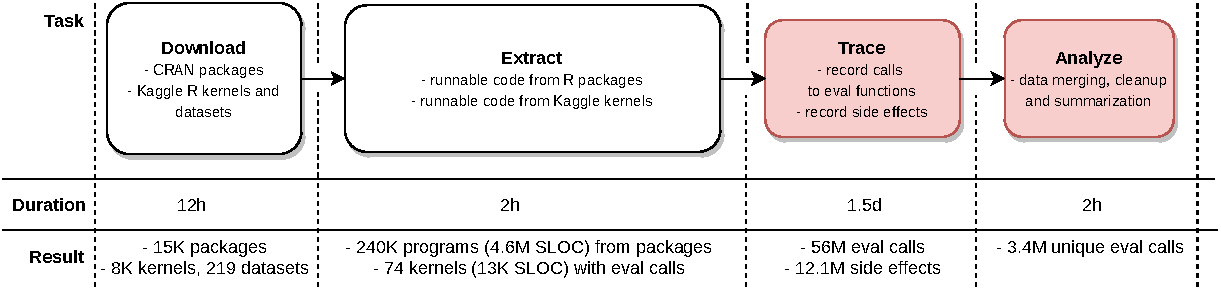
\includegraphics[width=.95\linewidth]{pipeline.pdf}
  \caption{Pipeline}\label{fig:pipeline}
\end{figure}

\medskip
\begin{compactenum}
\item \emph{Download.} Packages are downloaded from CRAN. For scripts, a web
  crawler retrieves code and the Kaggle command line tool gets data.
  Installation is complicated by native dependencies which are not properly
  documented and thus hard to automatically resolve.
\item \emph{Extract.} Given installed packages and scripts, the next step is to
  create runnable programs. The \genthat tool helpfully extracts all runnable
  code snippets from a package and turns each of these into a self-standing
  program~\cite{issta18}. Some Kaggle kernels are already scripts, for those
  nothing more needs be done. Others kernels are packages as notebooks, either
  as Rmarkdown or Jupyter, for those we use \c{knitr} to extract runnable code.
  The body of each extracted program is instrumented with calls to our dynamic
  analyzer to ensure that we only record calls to \eval from the code of
  interest and not from bootstrapping or execution harness operations.
\item \emph{Trace.} Each program is executing using our dynamic analysis tool
  which is a heavily instrumented interpreter that captures calls to \eval and
  many other fine-grained runtime events. Packages are run twice, once to
  capture \eval calls originating from package code, and a second time to
  capture calls coming from the base libraries. To avoid any interference, each
  program is run in its own process.
  As the GNU R bytecode compiler is written in R, we turn it off
  to avoid recording \eval in its code, and fallback on the interpreter.
\item \emph{Analyze.} Finally, analysis output is merged, cleaned and summarized
  in a post-processing phase driven by series of R scripts. The summarized data
  is then analyzed in RMarkdown notebooks to gather insights. All figures and
  numbers appearing in the paper are generated automatically. Figures are
  produced in PDF by \c{ggplot2}, numbers are exported as \LaTeX macros.
\end{compactenum}

\medskip\noindent The code extraction and tracing steps of the pipeline are run
in parallel~\cite{GNUparallel} orchestrated by a Makefile. Servers have
identical environments thanks to docker images with all dependencies installed.

\subsection{Dynamic Analysis}

The dynamic analysis is performed by \rdyntrace, a modified R virtual machine
based on GNU R 4.0.2 that exposes low-level callbacks for a variety of runtime
events~\cite{oopsla19b}.

The tracer registers callbacks to all \eval functions as well as a few other
ones that allow us to better identify where the expressions come from. For
example, we taint the results of calls to \c{parse} (turns string into
expression) and \c{match.call} (reflects on current call). We also capture calls
to R API for dynamic code loading (\eg\xspace \c{library}, \c{require} and
\c{source}). Next, we subscribe to the events related to a variable definition
and assignment allowing us to record side effects that happen in environments
while evaluating code in \eval. One challenge we encountered during the analysis
was that essentially R only provides source references for top-level calls in a
function body or in the block surrounded by braces. That is to say, a method
whose body would \c{eval(x)} would not have debug information that we can use to
identify that particular \eval. The same expression surrounded by braces would
have a line number and source reference. This is unfortunately not easily fixed
in the R implementation. Instead, we extended the dynamic analysis tool to
attach synthetic source code references to all \eval call sites by traversing
ASTs. The tracer is implemented as an R package in 3.2K C++ and 1.3K of R code.
For performance reason, most of the tracing is done in C++. While in theory the
implementation is rather straightforward, it is not so in practice:
%
\begin{compactitem}[---]

\item The lazy evaluation makes it difficult to analyze function arguments
  while tracing as prematurely forcing a promise might have dangerous
  consequences.

\item While the R interpreter is implemented in C, a lot of the core
  functionality is done in R. For example, package loading is implemented in R
  using \eval or the S4 and R6 object systems. This makes it hard in the tracer
  to separate the \eval that are essential to user programs from the
  accidental ones that are products of the way R implements its basic
  operations. This is even more so for the side-effects analysis.

\item In the dynamic analysis, we run all the \emph{runnable} code we obtained
  from CRAN and Kaggle---\ie real code written by people with highly varying
  expertise in R and programming in general. This exercises a lot of the corner
  cases of the highly underspecified R behavior.

\end{compactitem}


\mypara{Limitations.} The analysis has some limitation. Even with the extension
described above, there are still \PkgUndefinedRnd \eval calls without source
references. This occurs when a reference to the \eval function is passed as
argument to a higher-order functions or when the \eval call originates from
native code. However, these missing source references account for a meager
\PkgUndefinedRatio of all calls; they are unlikely to affect our results. Other
limitations are that we ignore calls to the native \eval function and to the
alternate \c{rlang::tidy\_eval} function which uses native \eval internally.
The \c{rlang} package introduces a new kind of promise called \c{quosure} which
is evaluated by \c{tidy\_eval}. None of these limitations should invalidate our
conclusions.

%%%%%%%%%%%%%%%%%%%%%%%%%%%%%%%%%%%%%%%%%%%%%%%%%%%%%%%%%%%%%%%%%%
\section{Usage Metrics}
%%%%%%%%%%%%%%%%%%%%%%%%%%%%%%%%%%%%%%%%%%%%%%%%%%%%%%%%%%%%%%%%%%

\begin{wrapfigure}{r}{5cm} \hspace*{-12mm}
  \centering
  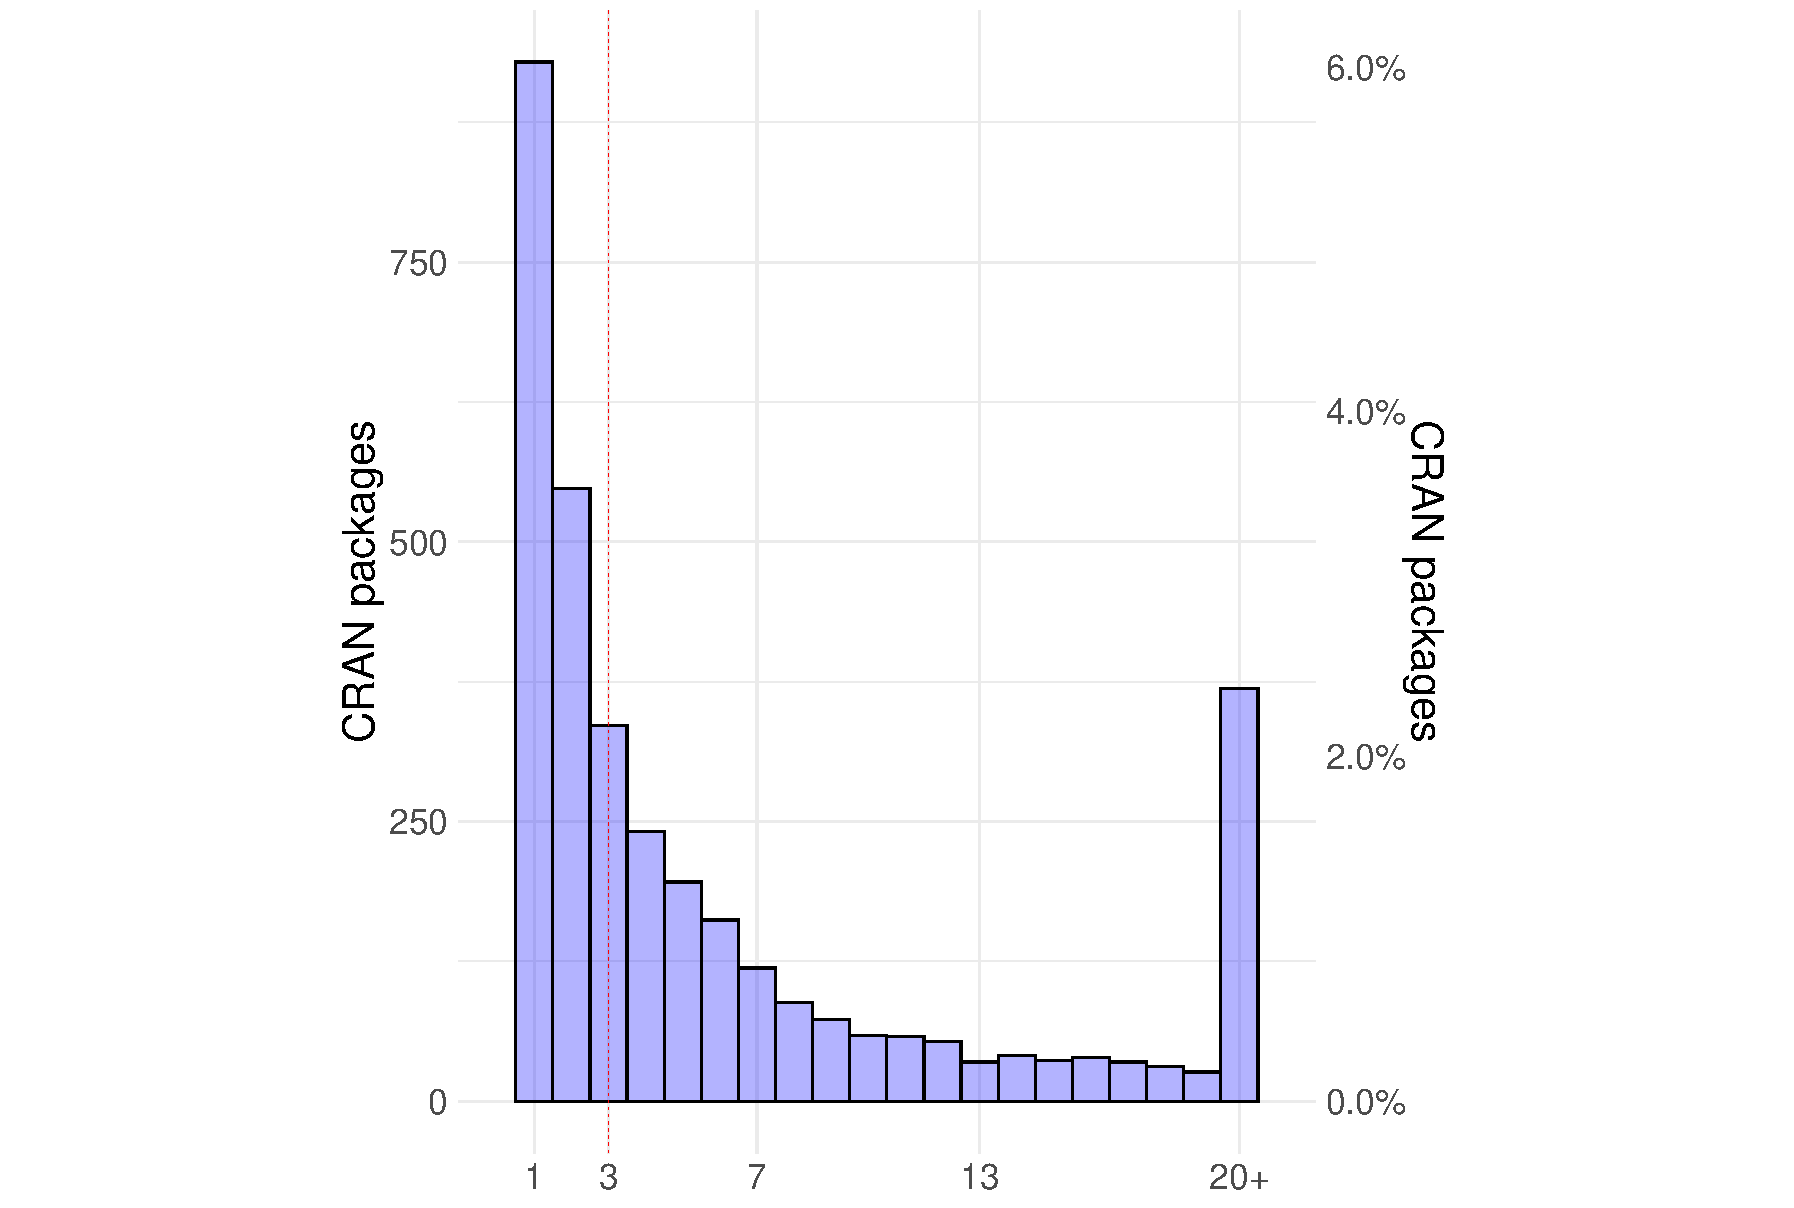
\includegraphics[width=72mm]{pkgs-eval-callsites-hist.pdf} \caption{CRAN
  \eval call sites}%
  \label{fig:pkgs-eval-callsites-hist}
\end{wrapfigure}
%
This section focuses on CRAN packages and reports statistics about the usage of
\eval. We use the word \emph{site} to an occurrence of a call site to the \eval
function in the source code, and \emph{call} to denote an observed invocation of
the \eval function.

\subsection{CRAN}

There are \PkgEvalCallSites \eval sites in \PkgPackages packages. The proportion
of packages calling \eval is \PkgPackagesRatio. Over half of these packages
have fewer than 3 sites, and with the exception \MaxEvalCallSitesPackage which
has \MaxEvalCallSitesCount sites, all packages contain fewer than
\MaxEvalCallSitesRest sites (\cf Fig~\ref{fig:pkgs-eval-callsites-hist} which
shows a histogram of sites per package). These sites appear in \PkgFunsWithEval
functions (\CranFunsWithEvalRatio of all functions in CRAN).


\begin{figure}[!b]
\small
\begin{tabular}{@{}l@{\hspace{1.5cm}}l@{}}
\begin{minipage} {5cm}
  \begin{tabular}{|r@{\,}r@{\,}l@{}r|r@{\,}r@{\,}l@{}r|} \hline
    \multicolumn{3}{|c}{\small\#calls} &\small \#pck
&     \multicolumn{3}{c}{\small\#calls} &\small\#pck \\\hline
\tt 1 &--& \tt 10      & \packageBina  & \tt 1K &--&\tt 100K  & \packageBine\\
\tt 11 &--& \tt 100    & \packageBinb  & \tt 100K &--&\tt 1M  & \packageBinf\\
\tt 101 &--& \tt 1K    & \packageBinc  & \tt 1M &--&\tt 10M   & \packageBing\\
\tt 1K &--& \tt 10K    & \packageBind  & \tt 10M &--& \tt 100M & \packageBinh\\\hline
\end{tabular}
\caption{Call frequency}\label{freq}
\end{minipage}
&
\begin{minipage}{7cm}
\begin{tabular}{|@{\,}r|rrrr|}\hline
  &\eval & \c{evalq} & \c{eval} & \c{local}\\[-2mm]
           & & & \c{.parent} &\\\hline
\small Static sites &\packageStaticeval&\packageStaticevalq&\packageStaticevalparent&\packageStaticlocal \\
\small Exercised sites&\packageTriggeredeval&\packageTriggeredevalq&\packageTriggeredevalparent&\packageTriggeredlocal\\
\small Invocations&\packageEvalsRnd&\packageEvalqsRnd&\packageEparentsRnd&\packageLocalsRnd\\\hline
\end{tabular}~\\[2mm]\caption{Variants}\label{tab:variantseval}
\end{minipage}\end{tabular}

%\end{figure}

%\begin{figure}[b] \centering
  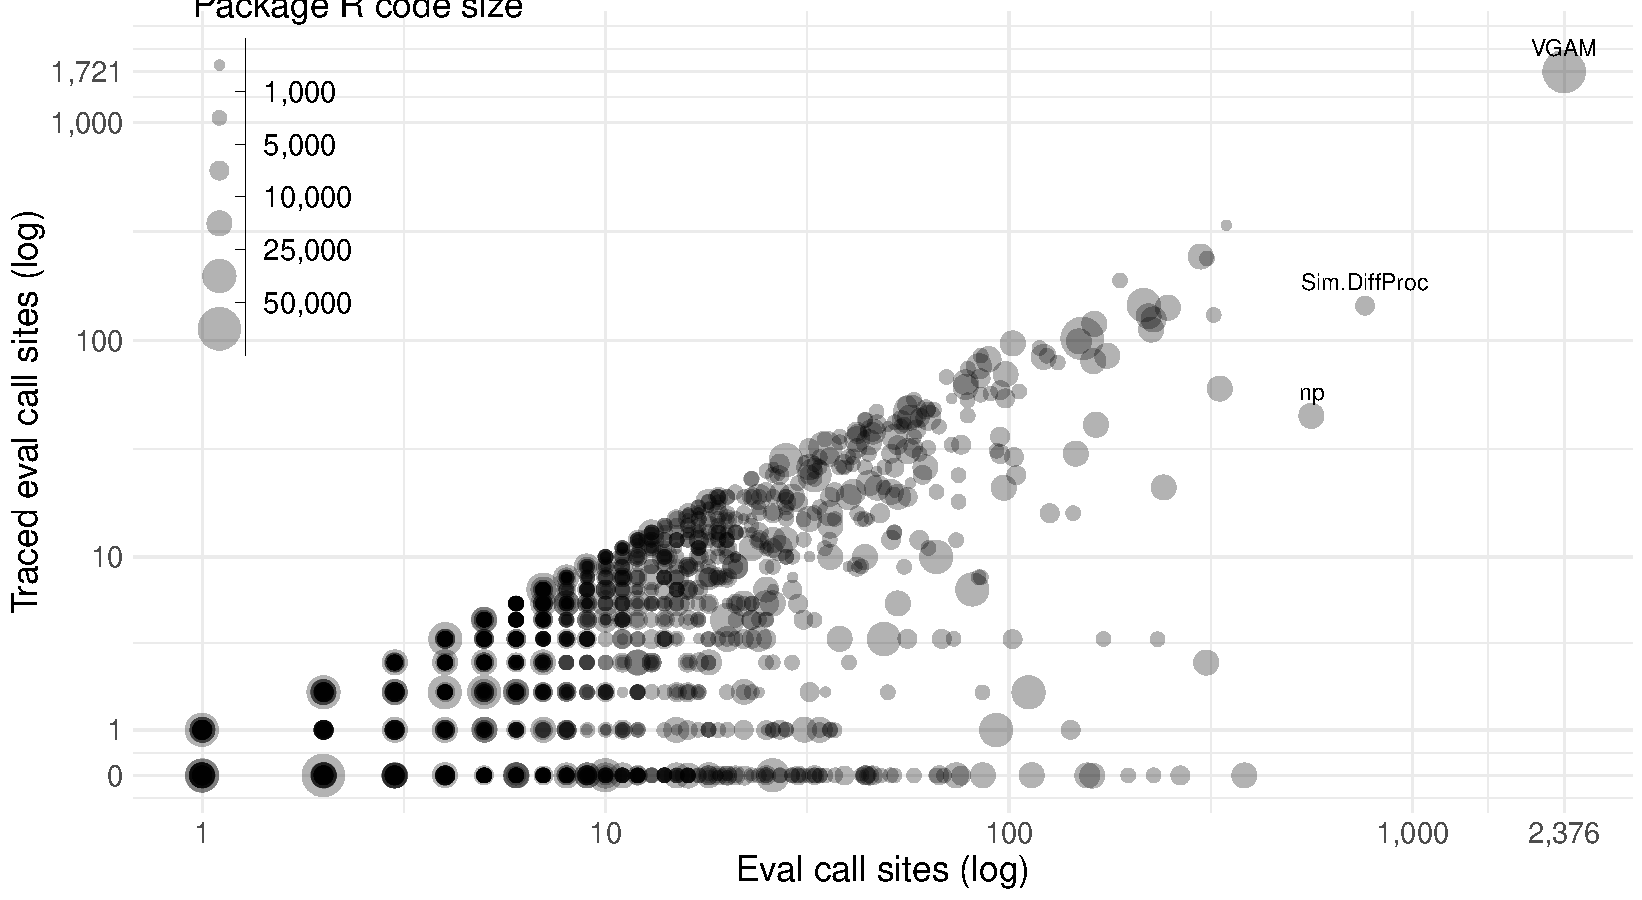
\includegraphics[width=.78\textwidth]{traced-eval-callsites.pdf} \centering
  \caption{\eval call sites coverage of the \PkgPackages packages.}%
  \label{fig:traced-eval-callsites}
\end{figure}


For dynamic analysis, we run \CranRunnableScripts programs extracted from
\CranPackages packages. Any run that does not exercise \eval is discarded. This
left \packageNbruns runs from \packageCorpus packages. There were
\packageAllcalls calls in \packageTriggeredpkgs packages originating from
\PkgHitEvalCallSites unique sites. In terms of coverage, the data exercised
\PkgHitEvalCallSitesAvgRatio of sites, a coverage similar to the code coverage
metric for the packages which is \PkgCodeCoverage. The fact that not all sites
are exercised can be chalked down to incomplete tests and occasional analysis
failures (\PkgFailedProgramsRatio of programs crashed or timed out).
Fig~\ref{fig:traced-eval-callsites} shows the number of sites that were
exercised; coverage is unequal. Figure~\ref{freq} summarizes the frequency of
dynamic calls to \eval with the left column being the number of calls and the
right, the number of packages in that range. There are \packageFewcalls packages
with low \eval frequency, fewer than 100 calls; and a smaller, but still
significant, number of packages, \packageManycalls to be precise, that use \eval
more than 1,000 times. Package \packageMaxcallspack makes \packageMaxcalls calls
and thus accounts for over half of the observations.
Figure~\ref{tab:variantseval} summarizes the use of variants of \eval. For each
of the four variants, the first rows shows the number of sites in the corpus
(\emph{static}), the second row is the number of sites that were encountered
during analysis (\emph{exercised}), the last row is the number of calls
(\emph{invocations}). The overwhelming majority of sites and calls, are to \eval
itself, \c{eval.parent} is rare, and both \c{evalq} and \c{local} are barely
used at all. The difference between sites and exercised sites underscores the
limitations due to code coverage.

\begin{wrapfigure}{4}{5.8cm}
  \vspace*{-2mm}
\centering
  \begin{tabular}{|r@{\,}r@{\,}l@{\,}r|r@{\,}r@{\,}l@{}r|} \hline
\multicolumn{3}{|c}{\small\#calls} &\small\#sites &
\multicolumn{3}{c}{\small\#calls} &\small\#sites \\\hline
\tt 0 &--& \tt 50    & \packageRunbina & \tt 501 &--& \tt 1000   & \packageRunbine\\
\tt 51 &--& \tt 100  & \packageRunbinb & \tt 1001 &--& \tt 1500  & \packageRunbinf\\
\tt 101 &--& \tt 250 & \packageRunbinc & \tt 1501 &--& \tt 2000  & \packageRunbing\\
\tt 251 &--& \tt 500 & \packageRunbind & \tt 2001 &--& \tt 3000 & \packageRunbinh\\\hline
\end{tabular}

  \medskip  (a) All  \medskip  \medskip

  \vspace*{-1mm}
  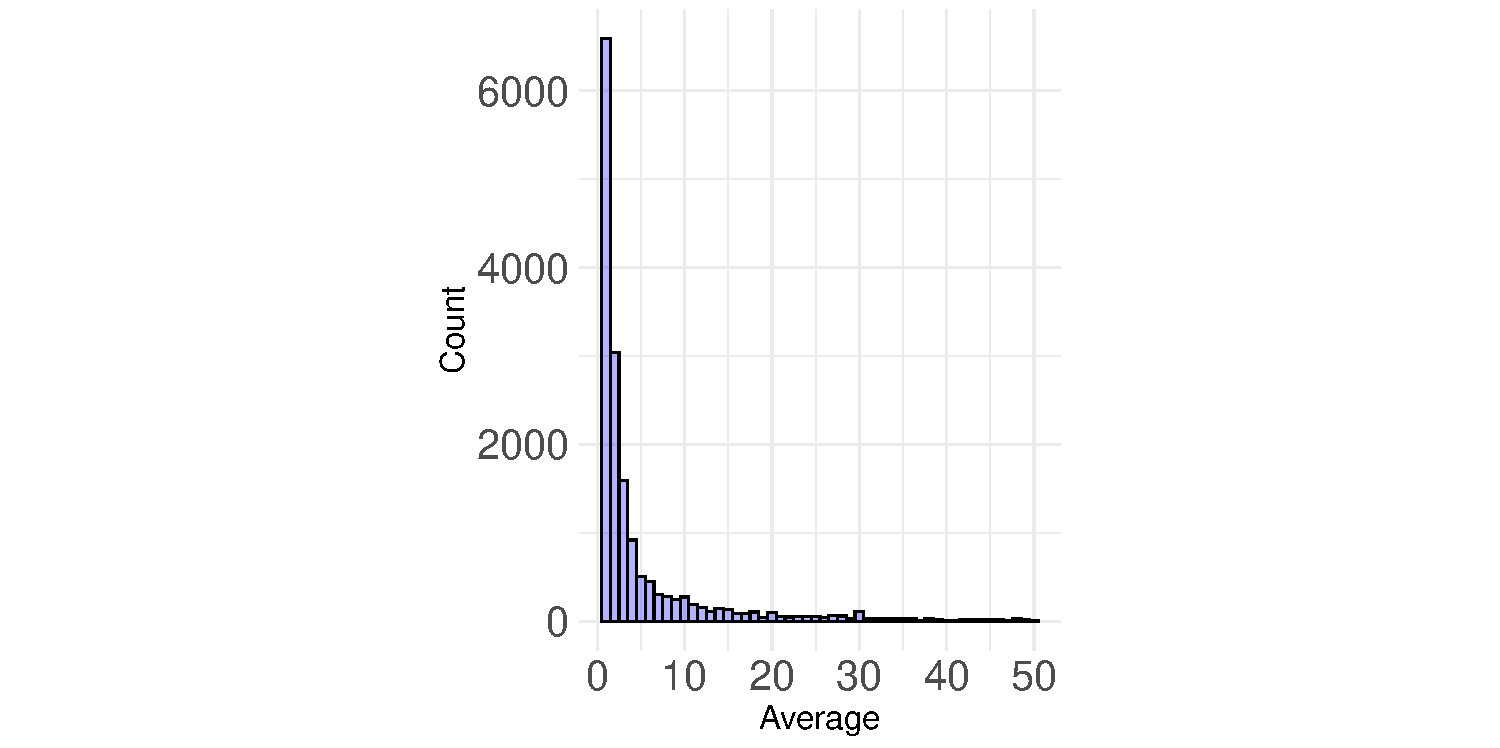
\includegraphics[width=5.6cm, trim=5.5cm 0 5cm 0, clip]{package_calls_per_run_per_call_site}

  (b) Small

\caption{Normalized calls} \label{cn}\vspace{-2mm}

\medskip
\medskip

\begin{tabular}{c}
  \vspace*{-1mm}
  {\hspace{-3cm}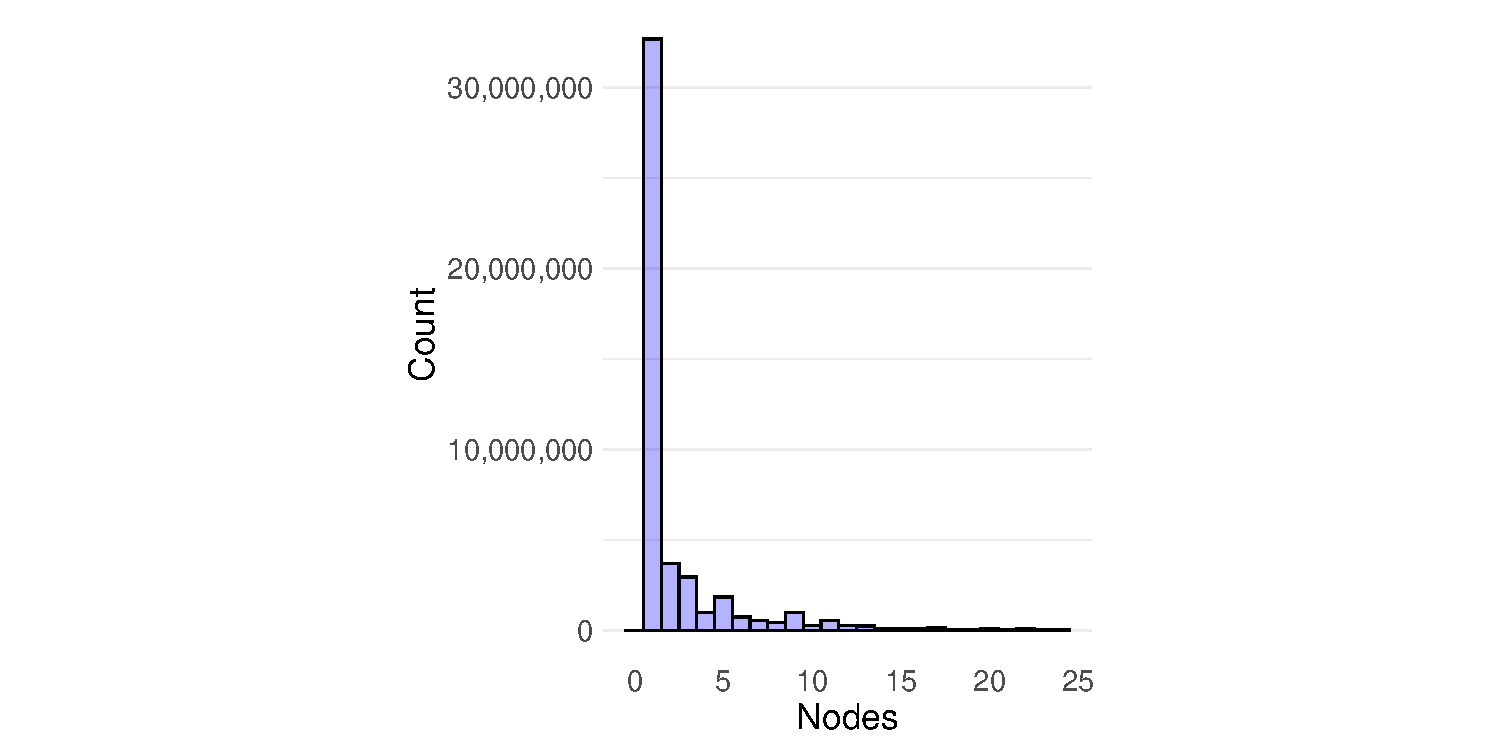
\includegraphics[width=0.8\textwidth]{package_size_loaded_distribution}}
\end{tabular}
 \caption{Loaded code} \label{fig:sizedistribution}
\end{wrapfigure}

Figure~\ref{cn}(a) shows normalized call counts per site; on the left are
average number of calls from a given site and given run, on the right are counts
of sites that fall in that range. For instance, \packageRunbinh sites are
invoked 2,000+ times per run. Larger numbers suggest loops or recursive contexts
-- this seems to be the exception as most \evals, \packageRunbina, are exercised
50 times or less. Figure~\ref{cn}(b) zooms in on low frequency sites. The x-axis
shows normalized calls and the y-axis is the number of sites for that value. Most
low-frequency \evals are invoked only once, about half as many are invoked
twice; after that the frequency quickly drops.

\Eval takes any value, but if its argument is not an expression, \eval returns
it unchanged. Expressions account for \packageCodepercent of arguments in our
corpus. More specifically, \packageSymbolpercent are \texttt{symbol}s (single
variables such as \c{x}), \packageLanguagepercent are \c{language} objects
(function calls such as \c{f(x)} or \c{x+1}), and \packageExpressionpercent are
\c{expression} objects (lists of expressions such as function calls or
symbols). Further inspection reveals that most symbols,
\packageGgplotsymbolpercent to be exact, come from a single site in the
\c{ggplot2} package and have the value \c{\_inherit}.\footnote{This models
inheritance in \c{ggproto}, one of the many object-oriented systems in
R that is used exclusively in the \c{ggplot2} graphics library.}

To estimate how much executable code is injected through \eval, we measure the number of nodes in the expressions; for example, \c{x+1} counts as 3. We
also measured string lengths of unparsed expressions, but these measurements
were dominated by the size of data objects which could range in the MBs. The
median argument size is \packageMedianszeval (due to the symbols) and the
average is \packageAvgszeval nodes. The largest \eval input observed is
\packageMaxszeval\,-- a significant chunk of code.
Figure~\ref{fig:sizedistribution} shows the distribution of sizes for arguments
of fewer or equal to 25 nodes. The x-axis is the size of arguments in number of
nodes, and the y-axis is the count of arguments with that size. The size drops
rapidly, with few observations larger than 15 nodes. The long tail is omitted
for legibility.

To estimate the work performed in \evals, we count instructions executed by the
interpreter. Most invocations perform relatively little work with
\packageSmalleventspct of \evals executing 50 or fewer instructions. The violin
plot of Figure~\ref{ev}(a) corresponds to \evals executing $\leq$ 50
instructions, it is dominated by trivial symbol look ups. Figure~\ref{ev}(b) has
the work-intensive \evals which go all the way to \packageMaxeventsRnd
instructions.

\begin{figure}[tb!]
\begin{tabular}{@{}c@{}c@{}}
\begin{minipage}{7.5cm}
 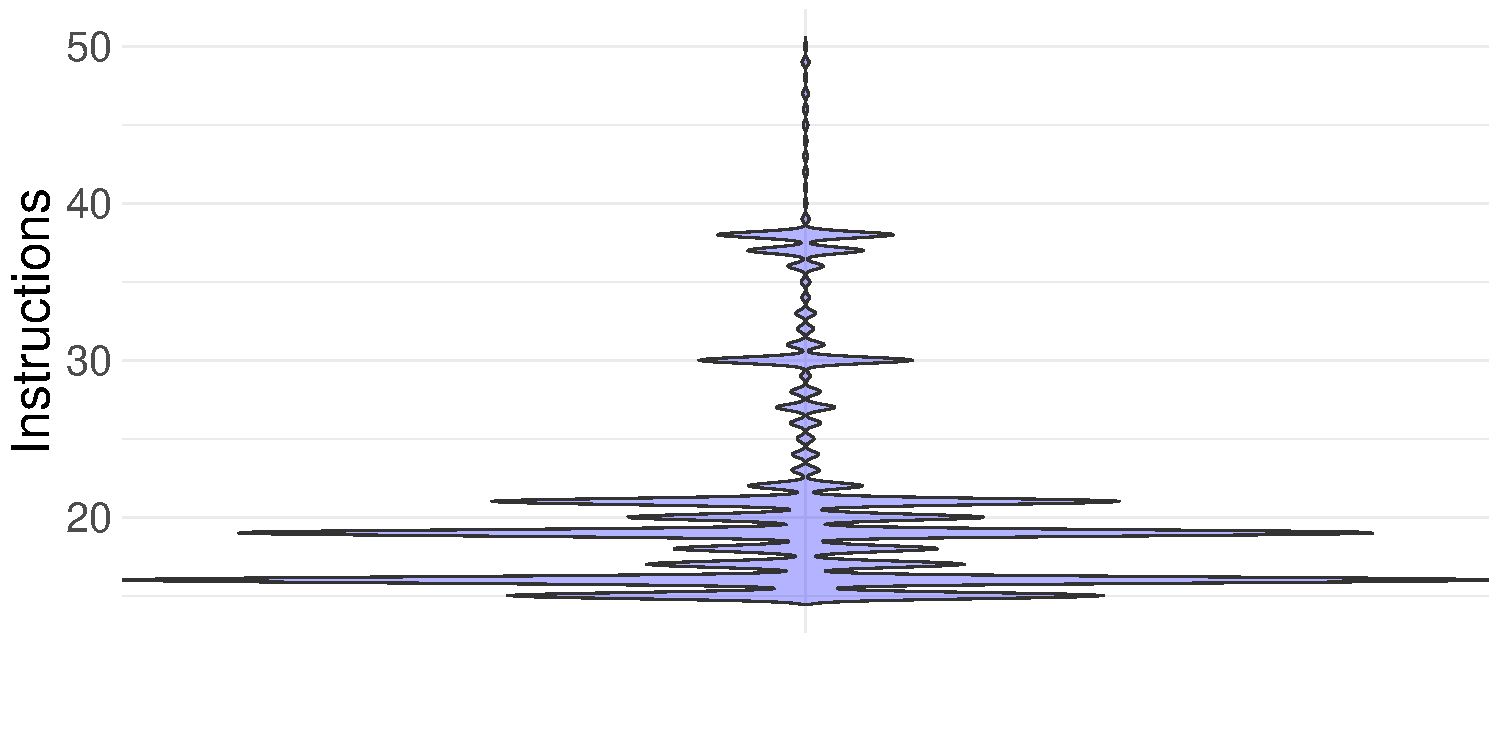
\includegraphics[width=\textwidth]{package_events_per_pack_small}
\end{minipage}&\begin{minipage}{7.5cm}
  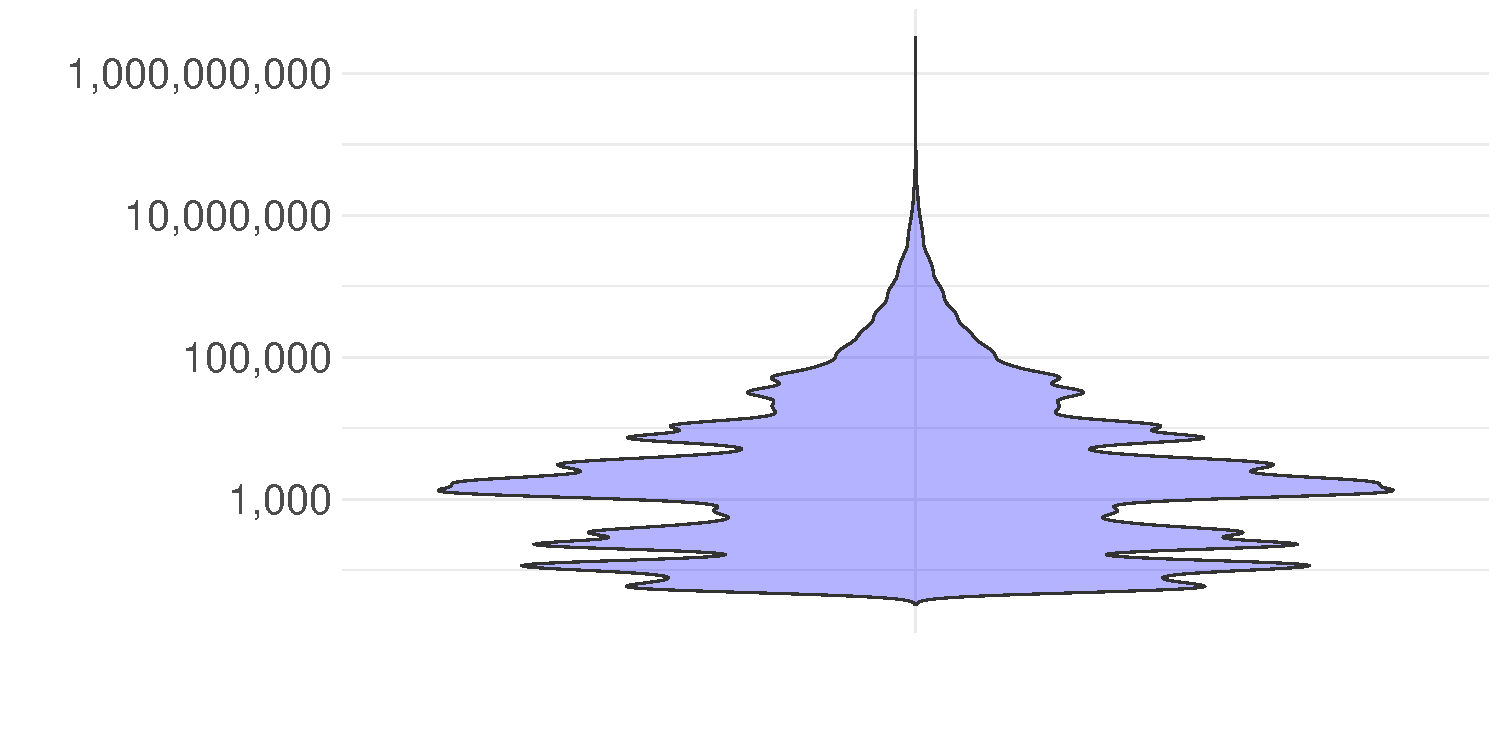
\includegraphics[width=\textwidth]{package_events_per_pack_large}
\end{minipage}\\[-3mm]
\small (a) Small & \small (b) Large
\end{tabular}
 \caption{Instructions per call} \label{ev}
\end{figure}

\subsection{Base}

We recorded \baseAllcalls \eval calls in the \BasePackages base libraries. This
comes from running 10\% randomly selected programs from the
\CranRunnableScriptsRnd extracted programs from CRAN packages, covering
\baseTriggeredevalpct of the \BaseEvalCallSites sites. Most of the calls
(\baseEvalsratio) are to the \c{eval} function and most arguments
(\baseCodepercent) are expressions. However, unlike CRAN, the majority
(\baseLanguagepercent) of the arguments are language objects. The median
argument size is \baseMedianszeval, which is more than for CRAN and the maximum
size is \baseMaxszeval, less than for CRAN. Small instruction counts ($<50$),
amount for \baseSmalleventspct of calls. A single site in the \c{match.arg}
function is responsible for \baseTopFuncPercent of all recorded calls. This
function provides a convenient way for argument verification using partial
matching. It is heavily relied on in R functions that use string arguments to
parameterize function behavior, a popular API mechanism in R. For example, in a
body of \c{center <- function(x, type = c("mean", "median", "trimmed"))} one
can get the value of \c{type} parameter using \c{type <- match.arg(type)}. A
call \c{center(x, "trim")} will match \c{type} to \c{"trimmed"}.

The challenge dealing with Base is that every program uses it. It can thus
generate extreme amounts of data but the data is quite predictable. For the
rest of the paper, we only mention Base when there are surprising
observations.

\medskip

\subsection{Kaggle}

In total, \kaggleAllcalls \eval were recorded, all to \eval function. Out of
\kaggleStaticeval sites from \KaggleWithEvals, only \kaggleTriggeredeval sites
in \kaggleNbruns scripts were hit. \KaggleFailedScripts scripts failed to run
and the other did not exercised the \eval sites. This is partially expected
as Kaggle code does not need to abide to any checks. Upon a manual inspection,
we observed that indeed the failing scripts were of a poor quality, often not
finished, using misspelled package names, hard-coded file paths or accessing
missing files.

Most call sites are invoked only once. Only one site is called \kaggleMaxcalls times.
Expressions amount for \kaggleCodepercent of arguments. Unlike CRAN corpus,
there are very few symbols (\kaggleSymbolpercent). Most expressions result from
calls to \c{parse}, thus most \evals start with strings. The median argument
size is \kaggleMedianszeval, which makes sense, as few arguments are only
symbols. The largest argument is \kaggleMaxszeval. The distribution of
instructions per eval is similar to CRAN; \kaggleSmalleventspct of \evals
execute fewer than 50 instructions. Manual inspection of \eval usage in Kaggle
suggest that it is consistent with the data obtained for CRAN. We do not
discuss it further.


\medskip

\subsection{Discussion}
These results show that \eval is central to the language implementation as it is
omnipresent in the relatively small Base library. The Base library is, in turn,
used by every single package. To avoid having Base dominate the result we have
excluded calls occurring there from the data we report when analyzing packages.
CRAN Packages, which are typically developed by experienced programmers, make
regular and varied use of \eval. They represent our most interesting data set as
these packages are the result of over 20 years of contributions by thousands of
authors. The code in packages is well maintained and relatively well tested.
Finally, Kaggle scripts are often written by less sophisticated users, and
likely perform simpler tasks, and thus have lesser need for \eval, and its uses
originate from strings as these are easier to manipulate for end-users. Due to
the relative paucity of data in Kaggle, we do not pursue the data set further.

%%%%%%%%%%%%%%%%%%%%%%%%%%%%%%%%%%%%%%%%%%%%%%%%%%%%%%%%%%%%%%%%%%%%%%%%%
%%%%%%%%%%%%%%%%%%%%%%%%%%%%%%%%%%%%%%%%%%%%%%%%%%%%%%%%%%%%%%%%%%%%%%%%%
\section{A Taxonomy of Eval}

The previous section gave a quantitative view of \eval usage; we now try to
elucidate \emph{what} it does.

\subsection{The expression in \eval} \label{sec:minimized}

The expressions passed to \eval vary widely. In order to categorize them, let us
use a minimization function $min(e)$ which for a given expression $e$ returns a
normal form that abstracts incidental details allowing the reader to focus on
the structure of the evaluated code. The minimization function performs constant
folding of arithmetic and string expressions for base operators, e.g.
$min(\c{1+1})=\c{V}$, value simplification, $min(\c{c(1,2,3+2)})=\c{V}$,
variable absorption, $min(\c{x+y})=\c{X}$, function absorption,
$min(\c{g(f(x),h(z))})=\c{F(F(X))}$ and a number of other simplifications.
Table~\ref{tab:minimizedexpressions} gives the 10 most frequent forms; \#sites
and \%sites are, respectively, the number and ratio of sites receiving arguments
of that form; \#packages is the number of packages with that form; \#operations
is the median number of instructions performed by the interpreter; and \%envir
is the ratio of sites that evaluate in a function environment. The example
column shows one sample expression $e$ that normalizes to the particular form.

\begin{table}[h]\small
\begin{tabular}{|c|r|r|r|r|r|c|}\hline
  $min(e)$& \#sites & \%sites & \#packages & \#operations & \%envir & example\\\hline
\c X&\packageMinimizedcallsitesa &\packageMinimizedpropsitesa &\packageMinimizedpackagea &\packageMinimizedmedianoperationsaRnd &\packageMinimizedpercentparentframesa & \c{y+1}\\\hline
\c{F(F(X))} & \packageMinimizedcallsitesb  & \packageMinimizedpropsitesb & \packageMinimizedpackageb  & \packageMinimizedmedianoperationsbRnd & \packageMinimizedpercentparentframesb & \c{gbov( mean(x), a-1)}\\\hline
\c{V}&\packageMinimizedcallsitesc &\packageMinimizedpropsitesc &\packageMinimizedpackagec &\packageMinimizedmedianoperationscRnd &\packageMinimizedpercentparentframesc& \c{c(42,21,0)}\\\hline
\c{F(X)}& \packageMinimizedcallsitesd & \packageMinimizedpropsitesd & \packageMinimizedpackaged & \packageMinimizedmedianoperationsdRnd & \packageMinimizedpercentparentframesd & \c{seq\_len(iters)} \\\hline
\c{\$} & \packageMinimizedcallsitese & \packageMinimizedpropsitese & \packageMinimizedpackagee & \packageMinimizedmedianoperationseRnd & \packageMinimizedpercentparentframese & \c{DF\$B}\\\hline
\c{model.frame}& \packageMinimizedcallsitesf & \packageMinimizedpropsitesf & \packageMinimizedpackagef & \packageMinimizedmedianoperationsfRnd & \packageMinimizedpercentparentframesf &  \c{model.frame(formula = Z $\sim$ U)}   \\\hline
\c{F()}& \packageMinimizedcallsitesg & \packageMinimizedpropsitesg & \packageMinimizedpackageg & \packageMinimizedmedianoperationsgRnd & \packageMinimizedpercentparentframesg & \c{rgamma(3, 2, n = 10L)} \\\hline
\c{FUN} & \packageMinimizedcallsitesh & \packageMinimizedpropsitesh & \packageMinimizedpackageh & \packageMinimizedmedianoperationshRnd & \packageMinimizedpercentparentframesh & \c{function(x, y) x + 3 * y} \\\hline
\c{<-} & \packageMinimizedcallsitesi  & \packageMinimizedpropsitesi & \packageMinimizedpackagei & \packageMinimizedmedianoperationsiRnd & \packageMinimizedpercentparentframesi & \c{x[1, 2:3, 2:3] <- value}\\\hline
\c{BLOCK} & \packageMinimizedcallsitesj & \packageMinimizedpropsitesj & \packageMinimizedpackagej & \packageMinimizedmedianoperationsjRnd & \packageMinimizedpercentparentframesj & \c{\{ write.csv(iris, tf) ; file.size(tf) \}} \\\hline
\end{tabular}
\caption{Minimized expressions} \label{tab:minimizedexpressions}
\end{table}

\noindent
We detail these forms and discuss their implication for the behavior of \eval.

\newcommand{\EE}[1]{{{\emph{\framebox{#1}}}}\\[1mm]}

\medskip\noindent\EE{$min(e)=\c{V}$} Expressions that represent values are
frequently passed to \eval -- they occur in 17\% of sites. The majority of
those, \packageValOneNodePercent, are inline constants (integer or double
vectors). The rest trivially evaluate to a value, \eg~\c{1+1}.\footnote{True as
long as base functions such as \c{+} are not redefined. They typically aren't,
but this is a limitation of this categorization.} In our corpus,
\packageNbCallSitesUniqueActualValue call sites only ever see a simple value.
Manual inspection reveals cases such as the following
\begin{lstlisting}
 f1 <- eval(paste("A~",paste(paste(names(X[,-1])),collapse="+")))
\end{lstlisting}
where the argument to \eval is a string which \eval simply returns. From twenty
randomly selected \evals, \packageUsefulValueEvalPercent of them do not need
\eval. For the other cases, either we are dealing with a value that needs to be
constructed dynamically or the value is a default case that sometimes is
replaced by a more interesting expression. This form is usually evaluated in few
interpreter steps, in fact the median is only
\packageMinimizedmedianoperationscRnd. The environment in which they evaluate is
mostly irrelevant (unless a built-in operator is redefined).

\medskip\noindent\EE{$min(e)=\c{X}$} Variables lookups are the most common form,
they are found in 28\% of the sites. This form includes simple variable reads,
\eg~\c{x}, those are \packageNbSymbolVarSitePercent of \c X. The form also
subsumes \c{V}, so it includes a mixture of arithmetic expressions,
\eg~\c{x+y+1}. The operations allowed are limited to built-in arithmetics. It is
noteworthy that, while most \c{X}\!s evaluate in a single step, the variable can
be bound to a promise, and accessing it may trigger evaluation of that promise,
thus resulting in an arbitrary amount of computation. The median number of
interpreted operations is \packageMinimizedmedianoperationsaRnd, suggesting that
it is not the common case. Lookups are often evaluated in constructed
environments, as few as \packageMinimizedpercentparentframesc of these
expressions are evaluated in a function environment.

\medskip\noindent\EE{$min(e)=\c{\$}$} This form extends \c X to include lookup
with the dollar operator, \eg~\c{x\$f}, and vector indexing, \eg~\c{x[42]} or
\c{x[[24]]}. As with \c X we allow arithmetics and values in this form. Lookup
occurs in 6\% of the sites. The interpreter evaluates
\packageMinimizedmedianoperationsgRnd operations on average; the minimum is 3
operations. This is typically used in a function environment,
\packageMinimizedpercentparentframese of the time to be precise.

\medskip\noindent\EE{$min(e)=$~\c{<-}} This form includes both assignments
operator, the direct assignment {\tt <-}, and assignment to the parent
environment {\tt <\,\!<-}, and the \c{\$} form. Assignments occur in 4\% of the
sites. They represent the most obvious source of side-effects. The median number
of operations is \packageMinimizedmedianoperationsiRnd; the minimum is 3.

\medskip\noindent\EE{$min(e)=\c{F()}$} This form captures simple function calls,
\eg~\c{f(2)}, with neither variables or assignments. Or, more specifically it
allows for variables in the function position but not in arguments. Usually,
looking up function names does not trigger computation, but that is not a given
if the function is returned by a promise or if the function name is shadowed by
a promise containing a value, then computation will occur. This form occurs in
6\% of sites and typically does not perform much work in the interpreter.

\medskip\noindent\framebox{$min(e)=\c{F(X)}$}~\EE{$min(e)=\c{F(F(X))}$} These
forms allow for function calls whose arguments may include variable references.
The latter allows nested calls.Assignments are excluded from this form. They
occurs in, respectively, 14\% and 20\% of the sites in the corpus. Together they
are the most frequent forms. The median numbers of interpreter steps are,
respectively, \packageMinimizedmedianoperationsdRnd and
\packageMinimizedmedianoperationsbRnd. The \packageMinimizedpercentparentframesj
of these expressions run in function environments.

\medskip\noindent\EE{$min(e)=\c{FUN}$} This form captures expressions define
functions, \eg~\c{function(x)x+1}, and do nothing else. \c{FUN} occurs in
\packageFunctionDefinitionSitesPercent of sites. Evaluating a function
definition is done in 2 interpreter step; the data does not record the work
performed by the interpreter when the generated functions are eventually run. In
addition to \c{FUN}, \packageGeneralizedFunctionDefinitionSitesPercent of sites
have function definitions nested in other expressions, this gives an idea of the
use of higher-order functions.

\medskip\noindent\EE{$min(e)=\c{BLOCK}$} This form captures multi-statements
code blocks, which occur in only 4\% of sites. These are larger expressions, we
do not inspect contents of the blocks. The median number of executed operations
is \packageMinimizedmedianoperationsjRnd. They typically run in function
environments.

\medskip\noindent\EE{$min(e)=\c{model.frame}$} The \c{model.frame} function
returns a dataframe that is the result of fitting the model described in a given
formula. This form subsumes \c{F(F(X))}, \c{FUN} and assignments. It is the
single most popular function invoked from \eval, it occurs in 7\% of the sites.
Each call does quite a lot of work with a 2K instructions median.

\paragraph{Consistency} It is interesting to consider how many different
forms any given site sees. The more forms, the harder it will be to characterize
the behavior of the program at that site. Luckily, \packageNbOneMinimizedPercent
of sites only see a single form. There are few sites that are highly polymorphic
(8 or more different forms), these include the pipe operator of the \c{magrittr}
package which is used to compose functions.

\paragraph{Discussion} The variety of uses of \eval is evidenced by the number
of different forms observed in CRAN. In comparison, JavaScript \eval usage was
simpler and more predictable as reported by \citet{oopsla12b}. Nevertheless,
simple forms dominate and there are many cases where \eval could be replaced
by less powerful constructs.


\subsection{The environments of \eval}\label{sec:env}

The environment in which evaluation happens determines what is visible to the
computation started by \eval and the potential reach of its side-effects. The
second argument to \eval specifies that environment. Environment of \eval can be
classified into the following four kinds:

\begin{compactitem}[---]
\item \emph{Function:} environment for the local variables of some function
  currently active on the call stack. Obtained by calling \c{parent.frame()} or
  \c{sys.frame()}.
\item \emph{Synthetic:} environments built from data structures such as lists,
  dataframes, or constructed explicitly with \c{new.env}, \c{list2env} or
  \c{as.environment}. Also includes the empty environment.
\item \emph{Global:} the environment in which scripts or interactive commands
  are evaluated.
\item \emph{Package:} the environment of a loaded library.
\end{compactitem}

\noindent
As shown by Table~\ref{tab:highlevelenvironments}, most calls evaluate in a
function environment with the \c{global} kind as a distant second. This means
that most variable lookups and most side effects either read/update existing
local variables or introduce new ones. But for which function? From the point of
view of the function that called \eval, Table~\ref{tab:funoffset} gives an
offset on the call stack. Thus 0 is the direct caller and corresponds to local variables; 1 is its parent, and so on. The data suggests that in 81\% of cases, \eval access its caller's environment -- this means, the variables of the function where \eval textually
occurs are read and written to. It is interesting that some 1.5\% of sites
evaluate a code in an environment that is three frame or above from \eval. This
distance implies that, in general, modular reasoning is impossible, to
understand the behavior of any piece of code entails fully understanding the
behavior of all functions that the code may call as the actions of \eval may
happen at a distance. Finally note that any particular site may have several
kinds of environments, but in \packageNbOneCategoryEnvirSitePercent of the case a
site has a single kind.

\begin{table}[h]
  \centering\small\hspace{-.5cm}
\begin{minipage}{3.7cm}
  \begin{tabular}{@{}r|r|r@{}}\hline
 Kind & \#sites & \%sites \\\hline
 Function & \packageNbFunctionEnvSites &  \packageNbFunctionEnvSitePercent\\
 Synthetic & \packageNbSyntheticEnvSites & \packageNbSyntheticEnvSitePercent \\
 Global &  \packageNbStrictGlobalEnvSites & \packageNbStrictGlobalEnvSitePercent \\
 Package & \packageNbPackageNamespaceEnvSites & \packageNbPackageNamespaceEnvSitePercent \\\hline
\end{tabular}
\caption{Kinds per site} \label{tab:highlevelenvironments}
\end{minipage}\hspace{-.2cm}
\begin{minipage}{3.7cm}\centering
\begin{tabular}{@{}r|r|r@{}}\hline
 Offset & \#sites & \%sites \\\hline
  \packageCallerEnvHierarchyNamea & \packageCallerEnvHierarchySitesaRnd & \packageCallerEnvHierarchySitePercenta \\
  \packageCallerEnvHierarchyNameb& \packageCallerEnvHierarchySitesbRnd & \packageCallerEnvHierarchySitePercentb \\
  \packageCallerEnvHierarchyNamec& \packageCallerEnvHierarchySitescRnd & \packageCallerEnvHierarchySitePercentc  \\
$\ge 3$& \packageNbFarAwayCallerSites &  \packageNbFarAwayCallerSitePercent \\\hline
 \end{tabular}
\caption{Function offset}\label{tab:funoffset}
\end{minipage}\hspace{-.2cm}
\begin{minipage}{3.7cm}
\begin{tabular}{@{}r|r|r@{}} \hline
Parent & \#sites & \%sites \\\hline
Function & \packageNewEnvCategorySitesa & \packageNewEnvCategorySitePercenta \\
Package & \packageNewEnvCategorySitesb &  \packageNewEnvCategorySitePercentb\\
Global & \packageNewEnvCategorySitesc & \packageNewEnvCategorySitePercentc \\
Empty & \packageNewEnvCategorySitesd & \packageNewEnvCategorySitePercentd \\\hline
\end{tabular}
\caption{Wrapper envs.} \label{tab:newenvs}
\end{minipage}\hspace{-.2cm}
\begin{minipage}{3.7cm}\centering
 \begin{tabular}{@{}c|c|c@{}} \hline
 \#kinds & \#sites &  \%sites \\ \hline
 \packageNbCategoryEnvira & \packageNbCategoryEnvirSitesaRnd &  \packageNbCategoryEnvirPercenta\\
 \packageNbCategoryEnvirb &  \packageNbCategoryEnvirSitesbRnd & \packageNbCategoryEnvirPercentb \\
 \packageNbCategoryEnvirc & \packageNbCategoryEnvirSitescRnd &  \packageNbCategoryEnvirPercentc\\
 \packageNbCategoryEnvird & \packageNbCategoryEnvirSitesdRnd & \packageNbCategoryEnvirPercentd\\\hline
\end{tabular}\caption{Multiplicities}\label{tab:polyenvir}
\end{minipage}\hspace{-1cm}
\end{table}

\noindent
Sites that evaluate in the global environment are likely split between
intentional and accidental use. Direct references to the top-level, using
\c{globalenv()} or \c{.GlobalEnv}, are rare, they occur in only
\packageNbExplicitGlobalSites sites. We suspect that the majority of uses of the
global environment come from the fact that our corpus consists of scripts that
are loaded at the top level, thus that environment may often be the caller of
\eval or close to it. The reason we make this point is that values stored in the
global environment are visible to all functions and are not reclaimed by the
garbage collector. So accidental uses may pollute that name space.

Synthetic environments need a parent. It is specified as an argument of the \c{new.env} function, or when \c{envir} is a list or a data frame, \eval uses its third argument
(\c{enclos}) as the parent.  The parent is used to lookup variables not found in its
child (side effects go to the child only). Table~\ref{tab:newenvs} shows the
kinds of the parents of synthetic environments. Over half are functions, then
come packages and global.


\paragraph{Discussion}
The data presented in this section is what one could expect. ({\it Function})
The majority of \eval call sites access the environment of some function on the
call stack. Usually, the current function, but sometimes frames arbitrarily far
up the call stack. One thing the data does not say is how that environment was
obtained. The expected case is that the environment was the one obtained from a
promise; as promises combine code and the environment in which that code
originates. Likely less frequent are cases where \eval is provided the results
of programmatically selecting some call stack. ({\it Synthetic}) The relative
high frequency of synthetic environments corresponds to cases when one wants to
evaluate an expression in either a restricted environment, use a data
structure as an environment. ({\it Global}) The fact that global environment
show up so frequently is likely an artifact of the way the code is run. ({\it
  Package}) There are only 92 sites that use a package environment in \eval,
this is probably best as it is bad form to add bindings or modify functions
of a loaded package. Many more sites rather wrap a package environment in a new
environment to create singletons in a package.

%% The \c{imchange} function of package \c{imager} makes it possible to modify
%% images using a dedicated formula syntax.\footnote{Inspired by {map} in
%% package \emph{purr}.} Here, \eval is evaluated in \c{newenv}, which creates a
%% new environment that inherits from \c{parent.frame()} by default (classified
%% as 1+).
%% \begin{lstlisting}
%%  newenv <- new.env()
%%  ...
%%  fo <- parse(text=as.character(fo)[2])
%%  im[where] <- eval(fo,envir=newenv,enclos=env)
%% \end{lstlisting}

%% \c{adjCoef} in package \emph{actuar} find the root of an equation defined by
%% a function \c{h} whose arguments must be named \c{x} and \c{y}. \c{h} is
%% transformed into an auxiliary function \c{h2} that can be optimized. Here,
%% the list used for \c{envir} ensures the correspondance between the textual
%% arguments of \c{h} and the arguments of \c{h2}.
%% \begin{lstlisting}
%%  sh <- substitute(h)
%%  fcall <- paste(sh, "(x, y)")
%%  ...
%%  h2 <- function(x, y)
%%  eval(parse(text = fcall),
%%  envir = list(x = x, y = y),
%%  enclos = parent.frame(2))
%% \end{lstlisting}

\subsection{The origins of \eval}

Where does the expression passed to \eval come from? There are various means of
creating that expression, these are associated with particular use cases, we
classify them in three categories:

\begin{compactitem}[---]
\item {\it Reflection:} This group corresponds to uses of the \c{match.call}
  function to reflectively capture the expression that invoked the current
  function.
\item {\it Constructed:} Expressions can be constructed by invoking the
  \c{quote}, \c{enquote}, \c{expression}. Function arguments are passed as
  promises and \c{substitute} is used to retrieve the source expression
  associated to the promise.
\item {\it String:} Finally, expressions can be created from strings by invoking
   \c{parse}, \c{str2expression} or \c{str2lang}.
\end{compactitem}

\noindent
Table~\ref{tab:provenance} summarizes the expression provenance in our corpus.
This data is obtained by dynamically tainting values as they are produced by the
various sources, due to technical reasons there is some imprecision in the
results. In particular, we are not able to classify all sites. Manual inspection
of numerous examples suggest that the classified results are accurate.

\begin{wraptable}{r}{5cm}\small\centering
\begin{tabular}{r|r|r} \hline
Origin  & \#sites & \%sites \\\hline
Constructed & \packageNbConstructedSites & \packageNbConstructedSitePercent \\
String & \packageNbStringSites & \packageNbStringSitePercent \\
Reflection &  \packageNbMatchCallExprsSites & \packageMatchCallExprsSitePercent\\\hline
\end{tabular}
\caption{Provenance}\label{tab:provenance}
\end{wraptable}

Strings could correlate with dynamic code loading. This is what the base
functions \c{source} and \c{sys.source} do. We observed few calls
(\packageNbParseFromFileSites in total) that consume the result of calling
\c{parse} on a file. Most of the calls build strings programmatically. We also
identified one function \c{invokeRestartInteractively} that prompts the user for
input, parses it, and passes it to \eval. The use of strings seems to correlate
with less sophisticated programmers; in our Kaggle corpus
\kaggleParseExprsSitePercent of site use strings.

\paragraph{Discussion}
The origin data suggests that constructing expressions from strings is a
minority of the use cases, instead the constructed category shows that the
majority of \evals comes code that was processed by the compiler, and may be
slightly modified by the programmer before invoking \eval. Both constructed and
reflection categories roughly correspond to meta-programming. Some of these use
cases could likely be replaced by macros if the R designers could be convinced
to overcome their distaste for those.

\subsection{Side effects in \eval}

The code executed by \eval can do side effects. From the compiler perspective,
we care about the observable side effects in environments---\ie variable
definitions, updates, and removals that are visible after a call to \eval
finishes. Knowing where---\ie in which environments do these side-effects
happen, can help us to determine how much of the compiler knowledge about the
program will be potentially invalidated.

The \rdyntrace contains low-level hooks capturing the life-cycle of an
environment and variables defined in it. In the tracer, we register callbacks
that record each environment creation and removal together with updates to its
bindings. From the recorded data, we ignore side effects
coming from \eval sites from unit testing frameworks.\footnote{In the corpus we
have \c{RUnit, testthat, tinytest} and \c{unitizer} unit testing frameworks.}
They run the testing code via \eval and thus the results would be biased
because of the high number of code run in these tests
(\CranRunnableCodeTestsRnd lines).

From the \packageNbrunsRnd programs we capture \SEAll side effects from
\SEAllCalls \eval calls in \SEAllSites sites. The challenge is again to remove
the accidental side-effects that are caused by the R virtual machine
implementation and are not related to the user code. For example, the
\c{.Random.seed} variable, which contains the state of the random number
generator is saved and restored from and to the global environment every time
user calls one of the base routines for getting random numbers. Removing them
leaves us with \SEUser side effects (\SEUserRatio) from \SEUserCalls \eval
calls (\SEUserCallsRatio) in \SEUserSites sites (\SEUserSitesRatio). These
sites are part of \SEUserFunctions in \SEUserPackages packages. \SEFunsNighty
functions are responsible for 90\% of side effects. Half of the side-effects
comes just from three functions: \c{plyr::allocate\_column} (allocates space
for a new data frame column), \c{withr::execute\_handlers} (executes deferred
expressions) and \c{foreach::doSEQ} (executes an expression on each element in
a collection, possibly in parallel).

Most of the \eval sites (\SESitesInEnvirRatio) do side effects in the
environment specified by the \c{envir} parameter (\cf
Section~\ref{sec:eval-in-r}), \SESitesNotInEnvirRatio modifies other
environment and finally \SESitesBothEnvirRatio does both.
Table~\ref{tab:se-env} shows the class of the environment where \eval side
effects happen (\emph{target environment}). It follows the classification
described in Section~\ref{sec:env} with two extra classes: \emph{Object} which
represents a side-effect that happens in S4 or R6 object environment, and
\emph{Local} that corresponds to a side effect in local variables of the \eval
caller. The table shows data for both \eval sites and functions. For a function
to have a given target environment class means that all of its \eval sites that
do side effect must have the same target environment class. Majority of the
\eval sites (\SESitesInOneClass) do all side effects consistently in one
environment class. The same happens on the function level. Almost half of the
sites and over a third of the functions do side effects in either \emph{Local}
or \emph{Object} environments. This gives a ray of hope for the compiler. Even
though it is possible to do anything anywhere, the data suggest that most
side-effects are sane.

\begin{table}[h]
  \small
  \centering
  \begin{tabular}{l|r|r|r|r}\hline
    Environments & \#sites & \%sites & \#funs. & \%funs. \\%
    \expandableinput tag/table-se-target-envs.tex
  \end{tabular}
  \caption{Most used target environments for \eval side-effects} \label{tab:se-env}
\end{table}

Table~\ref{tab:se-types} shows the proportion of the different side effects
that were recorded. In terms of calls we see mostly assignments and in terms of
sites definitions. This is expected. A subsequent \eval call will turn a
definition into an update. Variable removal, while rare, it does happen.
However, the vast majority comes from the already mentioned
\c{withr::execute\_handlers} function used to defer evaluation of an expression
to after the function exit. In our dataset, it is used almost exclusively by
the \c{tidyselect} package that uses it to remove the reference to current
quosure environment while interpreting a data frame column
selectors.\footnote{\cf \url{https://tidyselect.r-lib.org/}}

\begin{table}[h]
  \small
  \centering
  \begin{tabular}{l|r|r|r|r|r|r}\hline
    Side effect & \#events & \%events & \#calls & \%calls & \#sites & \%sites \\%
    \expandableinput tag/table-se-types.tex
  \end{tabular}
  \caption{Types of \eval side-effects} \label{tab:se-types}
\end{table}

\mypara{Discussion}
\todo{Is there any comparison with JS?}

\section{Usage of \eval}

\todo{Illustrate things that we have discussed in Section 5 - examples}
\todo{Things to discuss: model.frame, match.call, subset as example of NSE, substitute, parse, plots}


% We present here the main uses of \eval we have witnessed in R. Sometimes, they are design patterns, sometimes, \eval could be replaced by more specific functions. For each use of \eval, we discuss whether it is necessary to use.

% \subsection{Variable lookup}

% \eval is used to look-up the value of a variable in a given environment, different from the current scope so the \c{envir} argument of \eval is explicitly specified.

% \subsection{Metaprogramming}

% \mypara{\c{substitute}}

% \mypara{\c{match.call}}

% \todo{Talk about model.frame}

% \subsection{Logging}

% \subsection{Code transform}

% % Derivation of symbolic expressions

% \subsection{Plotting}

% \section{\eval expressivity and macros}

% The Thomas Lumley's article, Programmer's Niche: Macros in R, (https://www.r-project.org/doc/Rnews/Rnews_2001-3.pdf) describes how to write a `defmacro` function that would like as a macro creator, using `substitute` and `eval`.  There are no local macro variables in this implementation though.

The R language was intended to be extensible. The combination of lazy
evaluation, \c{substitute} and \c{eval} are the tools given to
developers to this end. This API is slightly more complex than just
passing a string, it is conceivable that this may discourage some
casual users. \Eval is also being used to reduce boilerplate code and
provide convenience features for programmers. We give examples for the minimized expressions of Section~\ref{sec:minimized} and then dig into high-level \eval design patterns.

\mypara{Variable lookup and values.}
This corresponds to minimized expressions \c{X}, \c{V}. We also include here lookup to slots in a list or data frame, \ie minimized expression \c{\$}.
It is the predominant usage of \eval in Base, through function \c{match.args}. In CRAN, it correlates with more exotic environments passed to \eval.

The dominant site in numbers of calls in CRAN, in the custom object system of \emph{ggplot2}, \c{ggproto}, also evaluates a variable \c{`\_inherit`} in the definition environment of the class. It leads to a large diversity of environments, many being package environment or package environments wrapped in \c{new}.

Package \emph{statnet.common} handles formulas, R object that associates an expression of the form \c{x ~ expr} and a carry-on environment where to evaluate the formula. It evaluates the left-hand side of the formula, which is always a variable, in \c{eval\_lhs.formula}, as \c{eval(object[[2L]],envir=environment(object))} where \c{object} is the formula and \c{environment} returns the formula associated to the object.


Slot lookup happens very often to evaluate some of the elements of a call list returned by \c{match.call}.
For instance in the \emph{pwrFDR} package:
\begin{lstlisting}
m <- match.call()
...
average.power <- m$average.power <- eval(m$average.power, sys.parent())
\end{lstlisting}

Here, \c{m\$average.power}, depending on the shape of the arguments to the surrounding function,  can be resolved to a variable, a more complex expression, or a number, leading to several possible minimized expressions, including \c{X} and \c{V}.

\mypara{Assigments.} It corresponds to minimized expression \c{<-} and groups together \c{<-}, \c{<<-} and \c{assign}. Package \emph{plyr} has a function combine data frames by row, filling in missing columns. During the allocation of the missing columns, an assignment call is built with \c{assignment <- quote(column[rows] <<- what)} and later evaluated on demand in a setter function, with \c{eval(assigmment)}. Package \emph{overture} is used to run Markov Chain Monte Carlo. It runs an R expression repeatedly and saves any assignments that happen, as samples of the Markov chains. 
The expression is captured with \c{substitute} and a new environment \c{env} wrapping the parent of the caller is created, in which all assignments will happen. Regularly, the content of \c{env} is inspected to sample the assigned variables.
\begin{lstlisting}
function(expr, overwrite=over.write) {
	expr_q <- substitute(expr)
	env <- new.env(parent=parent.frame(1))
	samps <- list()
	RunMcmc(samps, 1, expr_q, env, n.save, backing.path, thin, exclude, overwrite)
}

RunMcmc <- function... {
	 ...
	 eval(expr_q, envir=env)
\end{lstlisting}

\mypara{Domain Specific Language.} R expressions are built and transformed symbolically and then evalled to a concrete value. For instance,   base R packages \emph{stats} provides two operators for \emph{symbolic differentiation}, \c{D} and \c{deriv}. They support arithmetic operations and functions on real numbers such as \c{sin}.
In \emph{MCMCglmm} (Monte Carl Markov Chain Generalised Linear Mixed Models), a \c{Dtensor} object is created, which contains expressions derived twice (with \c{DD}) and then typically in a list or a data frame.
\begin{lstlisting}
 expr<-expression(beta_1 + time*beta_2+u)
 ...
 mu = data.frame(beta_1=0.5, beta_2=1, time=3, u=2.3)
 ...
 D[i]<-eval(DD(expr, name[unlist(comb.pos[i,])]), mu)
\end{lstlisting}
% See https://github.com/cran/MCMCglmm/blob/cfac9e67ec73a3db2142826faae35e5d2318da31/man/evalDtensor.Rd

Package \c{tidyselect} is the backend of several \c{dplyr} and \c{tidyr} functions to select columns. It offers a DSL that makes it possible to select a set of columns, over a range of columns, a complement, an intersection, an union, with a regular expression and so on. \eval is used to traverse selectors stored as slots of a dataframe.


\mypara{Capturing a call.}  A common use case for \eval is to be combined with \c{match.call}.
\c{match.call} walks up the call stack, captures the code that invoked the
currently executing function, and returns it as an unevaluated expression that includes the call function and its unevaluated arguments. The
pattern is to transform a call to some function \c{f} into a call to \c{g} with
some arguments retained and others modified.  \todo{or change the target
function. Both are described as "patterns" in the R documentation.} As an
illustration, consider the \c{vcpart} package's function \c{tvcglm} that is
translated to a call to \c{tvcm} with two modifications to the argument list:
argument \c{control} can't be missing and \c{fit} is set \c{"glm"}. The
function ends with a call to \c{eval.parent} to ensure that the rewritten call
is evaluated in the same environment the original call was.  \begin{lstlisting}
tvcglm <- function(formula, data, family, ...) { k <- match.call() k[[1]] <-
as.name("tvcm") if ("fit" %in% names(list(...))) warning("'fit' ignored.")
k$fit <- "glm" eval.parent(k) } \end{lstlisting} This pattern is recognizable
by the fact that the expression is a call and the target environment is that of
the parent.

% We have quantitative data on that if needed...
This pattern is very often (more than half of the cases) used in relation with statistical models, to build a new model, \c{model.frame} to build a new generic model, or a more specialized model like \c{glm} or, \c{lm}. The R documentation of \c{match.call} explicitly describes this usage.

In package \emph{survival}\footnote{It is a \emph{recommended package}, so recommended by the CRAN maintainers, thoroughly tested, and following R best practices.}, in function \c{coxph}, the surrounding call is first captured, then \c{model.frame} is injected as the function name in the call, and finally, the new call is evaluated in the parent frame.

\begin{lstlisting}
Call <- match.call()
...
tform <- Call[c(1,indx)]  # only keep the arguments we wanted
tform[[1L]] <- quote(stats::model.frame)  # change the function called
...
mf <- eval(tform, parent.frame())
\end{lstlisting}

A related pattern is not to change the call but rather to evaluate the arguments in the parent frame. This could also be achieved with \c{substitute}, but \c{match.call} does it in bulk.
In package \emph{MedDietCalc},  in function \c{computeMDS95}, \c{match.call} retrieves the argument expressions of the call, which are evaluated in a dataframe \c{data} which contains the numeric data. Each argument of function \c{computeMDS95} is also a column in dataframe \c{data}. The advantage of using \c{eval} here is to be able to express an argument as a combination of several columns in the dataframe.
\begin{lstlisting}
computeMDS95 <- function (data, Vegetables, Legumes, FruitAndNuts, Cereals,
	 Potatoes = NULL, Meat, Dairy, 	Alcohol, Fats = NULL, MUFA = NULL,
	  SFA = NULL, Sex, men = "male", women = "female", 	frequency = NULL,
	  output = "percent", rm.na = FALSE) {

	arguments <- as.list( match.call())
	Vegetables <- eval(arguments$Vegetables, data)
	Legumes <- eval(arguments$Legumes, data)
	FruitAndNuts <- eval(arguments$FruitAndNuts, data)
	Cereals <- eval(arguments$Cereals, data)
	Potatoes <- eval(arguments$Potatoes, data)
	...
\end{lstlisting}


In the R community, the call capturing pattern is often referred~\cite{hadley} as \emph{Non-Standard Evaluation}.

\mypara{Injecting code in package environments.} R distinguishes two kinds of environments for packages: the \emph{package} environment itself, which contains every publicly accessible functions, and the \emph{namespace} environment, which contains all functions including private ones.

 A call to \c{library(packageName)}, which loads libraries in R, for instance, will
populate environment \c{package:packageName} using \eval. It is a \emph{base} function
though, so we do not see it in the CRAN dataset. However, R still makes it
possible to access any package environments, which we see in
\packageNbPackageEnvPackages different packages in our corpus. Those packages perform
introspection, to represent and search any environment by name, in package
\emph{envnames}, to containerize tests, as with \emph{testthat} and
\emph{unitizer}, to create a custom OOP system with \emph{R.oo}, or to bypass the visibility of functions in \emph{USSCXenaTools}. It is also used to
implement a custom caching mechanism in packages \emph{g.data} and \emph{SOAR}.

\mypara{Code Generation.} The more traditional use of \eval is to execute code
that was assembled by the programmer into a string. Here we show the method
\c{plot} for class \c{sback} in package \c{wsbackfit}, simplified for
explanatory purposes. The function takes a long argument list, the names of
which are captured in the list \c{opt}. The string \c{stub} is composed of a
subset of the arguments passed to this function; the variable is used to
construct a call to \c{base::plot} which will draw a plot. \NOTE{This example
  is a bit messed up. What is var? Does the use of ... in the eval grab the
arguments of this call? If yes does it not end up with xlab twice? HELP}
\todo{Does this comment still applies?} The \parse and \eval combination is
used by the the \source function in the base library to load R code from a file
in the current workspace.  \begin{lstlisting} plot.sback <- function(x,...) {
opt <- names(list(...)) stub <- paste( ifelse("xlab" %in%
opt,"",paste(",xlab=\"",var,"\"",sep="")), ifelse("type" %in%
  opt,"",",type=\"l\""), sep="") plot <-
  paste("plot(x.data,",stub,",...)",sep="") eval(parse(text=plot))
  \end{lstlisting} This pattern is recognizable by its use of \c{parse} to turn
  a string into an expression.


\mypara{Debloating.} \todo{Wouldn't reducing boilerplate be a better name?} \Eval is often used as a means to reduce boilerplate code;
simple and repetitive code can easily be replaced with judicious use of \eval.
For example, the \c{data.table} package uses \eval to calls the \c{options}
function with named arguments taken from a vector of strings. While the benefits
are limited in this example, it is an attractive tool for programmers.
\begin{lstlisting}
  opts = c("datatable.verbose"="FALSE", # ...many others
  for (i in names(opts))
    eval(parse(text=paste0("options(",i,"=",opts[i],")")))
\end{lstlisting}
This pattern is a special case of code generation, recognizable by the
fact that \eval is executed in a loop.

\mypara{Trivial.} When values are passed to \eval, they are returned
unchanged. They are an example of trivial uses of \eval. Another
trivial use is the empty expression, often found in JavaScript, but
rare in R. \todo{Given that we do not have any data I would get rid of it}
\todo{We have the normalized expressions V and the small study I did on values passed to eval. And I did not find any eval() (empty) in the dataset. }

% Creating macros?

\mypara{Unnecessary use of \eval}

Similarly to JavaScript, there are also unnecessary uses of \eval. For example,
the \c{PerformanceAnalytics} package contains a function \c{chart.QQPlot} that
uses \eval to resolve a string into function and another to call it and assign
its results into a variable:
\begin{lstlisting}
function (R, d="norm", dp, ...) {
q.f <- eval(parse(text=paste("q",d,sep="")))
z <- NULL
eval(parse(text=paste("z<-q.f(",dp,",...)")))
}
\end{lstlisting}
  In both cases, there is no need for \eval:
\begin{lstlisting}
function (R, d="norm", dp, ...) {
q.f <- get(paste0("q",d))
z <- q.f(dp, ...)
}
\end{lstlisting}
or even to a oneliner \c{do.call(paste0("q",d), as.list(dp, ...))}.

\todo{Aviral's story when he contacted a developer about his use of eval}

\mypara{Discussion.} % more...

\eval is a powerful tool and can be sometimes with functions with more specialized goals. For instance, variable lookup in any environment can be performed with \c{get}, and assignment in any environment, with \c{assign}. Building a call and executing can be done with \c{do.call}. Nevertheless, \eval shines when expressions passed to it can be of many different types. % And it is shorter to type, and no need to remember all the specialized functions.

\section{Conclusion}

\bibliography{bib/bibliography,bib/jv}

\end{document}
